\documentclass[preprint,12pt]{elsarticle}

\usepackage{latexsym}
\usepackage{subcaption}
\usepackage{graphicx}
\usepackage{mathptmx}
\usepackage{placeins}
%
%****************************************************************************
% AUTHOR: You may want to use some of these packages. (Optional)
\usepackage{amsmath}
\usepackage{amsfonts}
\usepackage{amssymb}
\usepackage{amsbsy}
\usepackage{amsthm}
\usepackage{booktabs}
\usepackage{epsfig}

\usepackage{caption}
\usepackage{standalone}
\usepackage{tikz}
\usetikzlibrary{arrows}
\usetikzlibrary{decorations.markings}
\usetikzlibrary{calc}
\usetikzlibrary{shapes}

\usepackage{natbib}
\usepackage{fullpage}
\usepackage[linesnumbered,lined,ruled,commentsnumbered]{algorithm2e}

\newcommand{\specialcellr}[2][r]{%
  \begin{tabular}[#1]{@{}r@{}}#2\end{tabular}}

%****************************************************************************


%
%****************************************************************************
% AUTHOR: If you do not wish to use hyperlinks, then just comment
% out the hyperref usepackage commands below.

%% This version of the command is used if you use pdflatex. In this case you
%% cannot use ps or eps files for graphics, but pdf, jpeg, png etc are fine.

\usepackage[
  colorlinks=true,
  urlcolor=blue,
  citecolor=black,
  anchorcolor=black,
  linkcolor=black
]{hyperref}

%% The next versions of the hyperref command are used if you adopt the
%% outdated latex-dvips-ps2pdf route in generating your pdf file. In
%% this case you can use ps or eps files for graphics, but not pdf, jpeg, png etc.
%% However, the final pdf file should embed all fonts required which means that you have to use file
%% formats which can embed fonts. Please note that the final PDF file will not be generated on your computer!


%%\usepackage[dvips,colorlinks=true,urlcolor=blue,citecolor=black,%
%% anchorcolor=black,linkcolor=black]{hyperref}
%****************************************************************************


%
%****************************************************************************
%*
%* AUTHOR: YOUR CALL!  Document-specific macros can come here.
%*
%****************************************************************************
% Packages added manually
\usepackage{xcolor}
\usepackage{multirow}
%#########################################################
%*
%*  The Document.
%*
\begin{document}

\begin{frontmatter}


\title{Optimising Heterogeneous Ambulance Fleet Allocations in Jakarta}

\author[inst1]{Geraint Palmer}
\author[inst1]{Mark Tuson}
\author[inst1]{Sarie Brice}
\author[inst1]{Paul Harper}
\author[inst1]{Vincent Knight}
\author[inst2]{Leanne Smith}
\author[inst1,inst3]{Daniel Gartner}


\affiliation[inst1]{organization={School of Mathematics, Cardiff University},%Department and Organization
            addressline={Abacws, Senghennydd Road}, 
            city={Cardiff},
            postcode={CF24 4AG}, 
            state={Wales},
            country={United Kingdom}}
            
\affiliation[inst2]{organization={Welsh Ambulance Services NHS Trust},%Department and Organization
            addressline={Beacon House, William Brown Close}, 
            city={Cwmbran},
            postcode={NP44 3AB}, 
            state={Wales},
            country={United Kingdom}}

\affiliation[inst3]{organization={Aneurin Bevan University Health Board},%Department and Organization
            addressline={Lodge Road}, 
            city={Caerleon},
            postcode={NP18 3XQ}, 
            state={Wales},
            country={United Kingdom}}

%% Text of abstract  100-200 words

%A self-contained abstract of about 100-200 words outlining the aims, scope and conclusions of the paper must be supplied..
 \begin{abstract}
 Ambulance services have a duty of care to the clinical outcomes of the
 population they serve, and therefore aim to maximise the chances of survival
 and improve patient outcomes following a medical emergency. Despite this,
 although the ambulance location-allocation problem has been widely studied,
 it has predominantly focused on minimising response times or maximising
 coverage alone, and not explicitly for considering patient outcomes. In this
 paper we propose a modelling approach to consider where to optimally locate
 different types of emergency response vehicles in order to maximise patient
 outcomes within a heterogeneous population. To achieve this, we develop a
 heuristic algorithm for finding better fleet allocations which is used in
 conjunction with a discrete-event simulation model of ambulance services with
 heterogeneous vehicles. A major contribution of this heuristic is the numerical
 solution of a system of equations to be able to approximate the utilisation of
 vehicles. Traditionally this utilisation is problematic as it is both an input
 and an output of the allocation of vehicles. Our approach is informed by, and
 tested on, real-world data from Jakarta, Indonesia. Using our developed models,
 decision makers are better able to understand ambulance fleet capacity needs
 and locations, and their impact on patient outcomes.

\end{abstract}


%%Research highlights
% Please use 'Highlights' in the file name and include 3 to 5 bullet points (maximum 85 characters, including spaces, per bullet point).
\begin{highlights}
\item Mathematical modelling for maximising survival with heterogeneous
      patients and fleets
\item Population based neighbourhood search algorithm for finding better fleet
      allocations
\item Fixed point numerical solution to equation used to approximate utilisation
      of vehicles
\item A sequential simulation for ambulance demand and capacity planning
\item Application to Jakarta for policy recommendations and testing future
      demand scenarios
\end{highlights}

\begin{keyword}
% maximum of six keywords
%% keywords here, in the form: keyword \sep keyword
Ambulance Planning \sep Emergency Medical Services \sep Simulation \sep Health Care \sep Optimisation \sep Mathematical Modelling
\end{keyword}

\end{frontmatter}


\newpage


\section{Introduction and Background}\label{sec:intro}
Time-critical conditions (TCCs) are a substantial cause of mortality
worldwide, responsible for an estimated 54\% of all deaths \cite{FraserBMJ}.
Emergency medical services (EMS) play a pivotal role in responding to TCCs and
saving patients from life-threatening medical conditions. Most EMS research,
especially  planning to meet increasing ambulance demands, tends to be
focussed on high-income countries including, for example, Australia
\cite{lowthian2011increasing}, Germany \cite{veser2015demographic}, and USA
\cite{birmingham2021trends}. In contrast, most low and middle-income countries
(LMICs) lack an organised EMS system, with most ambulances used purely for
patient transport and not as an emergency care vehicle \cite{plummer2017ems}.
However, the burden of deaths due to TCCs is much greater in LMICs than in
high-income countries, the difference being around threefold \cite{ChangPMC}.
For traffic accidents, strokes and heart attacks, rapid access to appropriate
treatment is especially vital. 

The application of our research is focused on Indonesia, as supported by an
award for Global Challenges Research Funds (GCRF). In Indonesia, an LMIC,
there has been very little prior work on developing an EMS strategy, driven
largely by inadequate resources including a lack of financial investment and
human capital \cite{plummer2017ems,pusponegoro2003terrorism,yusvirazi2018state}.
Related research by the authors \cite{BriceSyaribahNoor2022Esui} has
highlighted particular challenges in Indonesia as a lack of a single
coordinated EMS, the ability or willingness to pay for an ambulance, a large
geographical area, and areas of severe traffic congestion especially in
Jakarta, the capital.  

When our research programme commenced in October 2019, ambulance services in
Jakarta were provided by many disparate, mostly private providers that charge
patients for their use, such as private hospitals. We initially partnered with
Ambulans 118, a non-government charitable ambulance service established in
2005 by the Indonesian Surgeons’ Association, that  currently operates in five
cities across Indonesia: Jakarta, Palembang, Yogyakarta, Surabaya and Makasser.
Unlike private providers, Ambulans 118 suggests that a donation is made for
use of its EMS vehicles, but otherwise provides free emergency medical care
and is also leading on paramedic training across the country. 

The overarching goal of our research was to work with the Indonesian
Government, the different ambulance providers, and hospitals, to help them
forecast emergency demand and make critical decisions on the optimal types,
capacities and geographical locations of emergency vehicles within a
potentially co-ordinated EMS system, starting with Jakarta. To facilitate
this, in collaboration with Ambulans 118 we organised workshops in Jakarta in
February 2020, thankfully just before the COVID-19 pandemic and lockdowns,
which were attended by over 170 people including doctors, nurses, paramedics,
academics, and officials from the Indonesian Ministry of Health. This paper
presents some aspects of the overall research programme, specifically focusing
on the development of a simulation model and location-allocation heuristics
for maximising patient survival.  

Fundamental to the project and the research described in this paper was an
initial study that we carried out in order to better understand patient needs
and the barriers to use of ambulances in Indonesia. Throughout the month of
December 2020, we undertook comprehensive surveys in Emergency Departments
(EDs) across Jakarta and published the first known study in to EMS demand
within the country \cite{BriceSyaribahNoor2022Esui}. Our study showed that the
utilisation of ambulances by patients attending EDs is considerably low and of
concern. The low utilisation is contributed to patients’ lack of awareness of
available ambulance services given a lack of coordination, patients’
disinclination to use ambulances due to high costs, and long response times.
All of these barriers impact on patient outcomes, especially for those with
life-threatening conditions. For example, remarkably more trauma patients took
a car-share ride (20\%) or motorcycle (20\%) to reach the ED than an ambulance
(just 10\%), while only 14\% of critical cardiovascular patients used an
ambulance compared to 67\% travelling to hospital by private car or a
car-share ride.

The first contribution of this paper is an extension the work of
\cite{Knight2012918} to consider both heterogeneous patients and heterogeneous
fleets. Here a maximal survival objective is formulated, from vehicle
allocations and utilisations, which are themselves found by numerically
solving a relationship on the vehicles' share of the demand. This is then used
in a heuristic to find allocations that maximise patient survival.
Secondly, we the develop of a comprehensive sequential discrete event EMS
simulation that models and evaluates heterogeneous fleet allocations of
emergency vehicles by utilising a novel approach in which transit jobs, rather
than patients, are framed as the queueing `customers'. Our methodology
utilises two discrete event simulations of the same system that are run
sequentially and together combine to form the logic of a single simulation of
a heterogeneous fleet; and key performance indicators (KPIs) are calculated by
making use of survival functions.
Thirdly, we demonstrate the use and impact of our modelling framework applied
to current and proposed ambulance allocations in the city of Jakarta, thus
supporting Government-level decision making with an overall goal to improve
the lives of those living in LMICs. This leads to decision support and
managerial insights in Indonesia, although the developed modelling framework
could be readily applied to other locations.

The paper is structured as follows:
Section~\ref{sec:litreview} gives an overview of the literature on modelling
ambulance allocations.
Section~\ref{sec:optimising} describes an
optimisation model, including the survival objective, utilisation
considerations, and a heuristic algorithm to find better fleet allocations.
Section~\ref{sec:simulation} outlines the logic of the sequential discrete
event simulation models for heterogeneous fleets.
Section~\ref{sec:jakarta} gives a case study, describing the current emergency
service situation in Jakarta and applying the optimisation and simulation
results.
Section~\ref{sec:discussion} discusses the findings and contributions of the
paper.



\section{Literature Review}\label{sec:litreview}
There is a rich literature on Operational Research applied to EMS location and
related allocation problems. Literature reviews that include these topics are
\citet{aringhieri2017emergency, belanger2019recent, farahani2019or, Li2011, Liu2021, reuter2017logistics}
and \citet{wang2021emergency}.

Emergency medical services can be evaluated using different performance
measures with coverage and response time being the predominant metrics
\cite{Mclay2010evaluating}. However, missing a response time target by just
one second, for example, would be considered as a `failure' in many models
with no appreciation at all of the impact on patient survival or outcome
\cite{Mclay2010evaluating}. This seems somewhat restrictive and short-sighted,
which is why we focus on survival as a metric and thus, in the following,
compare and contrast papers using that metric with our approach.

Table \ref{tab:RelatedWork} provides an overview of recent research that focus
on the survival metric. We break down related papers into discrete event
simulation~(DES), queueing theory and optimisation methods, and we provide a
summary of each paper from the table as well as compare and contrast them with
our modelling and solution approach.

\begin{table}[htbp]
\centering
\small
\resizebox{\textwidth}{!}{%
\begin{tabular}{llcccc}
\toprule
Reference   & Year & DES & Queueing Theory & Optimisation \\
\midrule
\citet{amorim2019integrated} & 2019 &  & & \checkmark \\
\citet{boutilier2022drone} & 2022 &  & \checkmark \\
\citet{Erkut200842} & 2008 & & & \checkmark\\
\citet{Knight2012918} & 2012 & & \checkmark & \checkmark \\
\citet{MCormack2015} & 2015 & \checkmark & & \checkmark\\
\bottomrule
\end{tabular}%
}
\caption{Break down of related research that focuses on survival.}
\label{tab:RelatedWork}
\end{table}

\FloatBarrier

\citet{amorim2019integrated} propose an integrated strategic and tactical
planning approach which features an optimization model and a local search
heuristic based on Gaussian Processes. Their methodology is applied to the
city of Porto while reporting on performance metrics such as survival. Our
approach is different because we use a discrete-event simulation framework and
a cross-entropy optimisation approach to determine the number of ambulances
required in each station. 

\citet{boutilier2022drone} develop an integrated location-queueing model that
incorporates existing EMS response times in a drone network. They use a
p-median approach and an Erlang loss model. Although survival is not their
main optimization criterion,  they report how many patients would survive
using their approach.

Erkut et al.~\cite{Erkut200842} can be considered the first modelling approach
that considers decaying survival probabilities during response time. The
rationale is, because survival can be thought of as a more robust and generic
objective for EMS performance measurement than coverage or average response
time. In an application of a recently developed Maximal Survival Location
Problem model (MSLP), the authors use data from Edmonton, Canada and show that
maximising survival is superior to other objectives in clinical outcome for
cardiac arrest patients.

McCormack and Coates~(2015)~\cite{MCormack2015} focus on the optimization of
EMS vehicle fleet allocation and base station location through the use of a
genetic algorithm (GA) with an integrated EMS simulation model. Their
objective is maximization of the overall expected survival probability across
patient classes. Applications of the model were undertaken using real call
data from the London Ambulance Service. The difference between their modelling
approach and our is that we have a different survival function, focus on a
different heuristic optimization and evaluate our approach with data from a
development country and have higher traffic volume and congestion in our data. 

Knight, Harper and Smith \cite{Knight2012918} provide a supporting extension
of the MSLP that allows it to be applied more generally to real-world EMS
systems, acknowledging that different patients have varying levels of expected
survival probabilities.  The Maximum Expected Survival Location Model for
Heterogeneous Patients, MESLMHP, allows multiple classes of patient groups to
be defined, where previously only cardiac arrest patients formed part of the
objectives for primary response. In reality, by definition any emergency
patient has a necessity for swift attendance, and a timely response to any
incident type may impact on clinical outcome in some way. It is for this
reason MESLMHP is designed to be generic enough to accommodate any number of
patient groups, with each class weighted dependent upon the relative urgency
of the incident.  More than just a contribution to the model’s demand input,
these patients are included in the optimisation when maximising total
population survival probability.


\section{Problem Statement \& Notation}\label{sec:problem_description}
We first present some notation. We have the following sets:

\begin{itemize}
  \item $\mathcal{P}$ is the set of pick-up locations, indexed by $p$;
  \item $\mathcal{A}$ is the set of ambulance locations, indexed by $a$;
  \item $\mathcal{K}$ is the set of medical specialities, indexed by $k$;
  \item $\mathcal{Y}$ is the set of hospitals, indexed by $y$.
\end{itemize}

To incorporate heterogeneous fleets the set of specialities $\mathcal{K}$ is
partitioned into two sets, $\mathcal{K}_A$, those patients that can be seen by
secondary vehicles, and $\mathcal{K}_B$, those patients who are seen by
primary vehicles only.

An allocation is given by the tuple $\left(Z_a, \tilde{Z}_a\right)$, where $Z_a$
is the number of primary vehicles allocated to ambulance location $a$; and
$\tilde{Z}_a$ is the number of secondary vehicles allocated to ambulance
location $a$. Also let:

\begin{itemize}
  \item $\lambda_{pk}$ be the rate at which patients of speciality $k$ make
        calls from pick-up location $p$;
  \item $s_k(t)$ be the survival function function associated with patients of
        speciality $k$;
  \item $\pi_a$ be the average utilisation of primary vehicles stationed at
        location $a$;
  \item $\tilde{\pi}_a$ be the average utilisation of secondary vehicles
        stationed at location $a$.
  \item $b_{pa}$ be the expected travel time from ambulance location $a$ to
        pick-up location $p$; and let $B_{pa}$ be a random variable representing
        the time it takes for an ambulance to drive this distance;
  \item $C_{py}$ be a random variable representing the travel time from pick-up
        location $p$ to hospital $y$;
        time it takes for an ambulance to drive this distance;
  \item $D_{ya}$ be a random variable representing the travel time from hospital
        $y$ to ambulance location $a$;
  \item $F_{pa}$ be a random variable representing the travel time from pick-up
        location $p$ to ambulance location $a$;
  \item $G_k$ be a random variable representing the time the ambulance spends
        with patients of speciality $k$ at the pick-up location;
  \item $J_k$ be a random variable representing the time the ambulance spends
        with patients of speciality $k$ at the hospital;
  \item $\Theta$ be a random variable representing the time the ambulance spends
        re-fuelling, re-stocking, and resting between transit jobs;
  \item $q_{pky}$ be the probability that a patient of speciality $k$ from
        pick-up location $p$ is taken to hospital $y$.
        Note that $\sum_{y \in \mathcal{Y}} q_{pky} < 1$ is possible, that is a
        patient may not go to any hospital, in which case the ambulance returns
        to their ambulance location.
\end{itemize}

To incorporate heterogeneous vehicles, let also $\tilde{\pi}_a$ denote the
average utilisation of secondary vehicles stationed at location $a$; and
$\tilde{b}_{pa}$, $\tilde{B}_{pa}$, $\tilde{C}_{py}$, $\tilde{D}_{ya}$, and
$\tilde{F}_{pa}$ denote the corresponding travel times for secondary vehicles.

Patients will call an ambulance from one of the pick-up locations
$p \in \mathcal{P}$. If \textit{all} ambulances are busy, then that call will be
abandoned and it is assumed that the patient will find their own way to the
hospital through private or public transportation. Otherwise, a central control
centre will dispatch the closest available primary vehicle. That vehicle will
travel from its location to the patient ($B_{pa}$), spend some time on the scene
treating the patient ($G_k$), travel to the hospital ($C_{py}$), spend some time
handing over the patient at the hospital ($J_k$), travels back to it's original
location ($D_{ya}$), then spends time refilling and refuelling ($\Theta$).
There is also a probability that the patient does not need a hospital, and so
the vehicle will travel from the pick-up location back to it's original vehicle
location ($F_{pa}$). These routes are shown visually in
Figure~\ref{fig:travel_routes}. Note that $B_{pa}$ and $F_{pa}$ need not
necessarily be equal, as travel times need not necessarily be symmetrical.

\begin{figure}
    \centering
    \includestandalone[width=0.65\textwidth]{img/diagram}
    \caption{Ambulance routes for a given transit job.}
    \label{fig:travel_routes}
\end{figure}

Therefore the total time an ambulance is busy will be $T_{paky}$ given by
Equation~\ref{eqn:service_time_withhosp} if a hospital is required, and
service time $T_{pak}$ given by Equation~\ref{eqn:service_time_nohosp} if no
hospital is required.

\begin{align}
T_{paky} &= B_{pa} + G_k + C_{py} + J_{yk} + D_{ya} + \Theta \label{eqn:service_time_withhosp} \\
T_{pak} &= B_{pa} + G_k + F_{pa} + \Theta \label{eqn:service_time_nohosp}
\end{align}


\section{Optimising Allocations for Maximal Survival}\label{sec:optimising}
Here we outline a method of finding vehicle allocations that that maximise the
expected survival of patients.
We assume that there are two types of vehicle: primary vehicles, typically
ambulances, that must be dispatched to all patients; and secondary vehicles,
typically rapid response motorcycles, that can travel faster than primary
vehicles, and are dispatched to some patients to respond to an emergency
faster than the primary vehicle. Secondary vehicles cannot transport patients,
but are used in conjunction with primary vehicles to reduce response times.
The problem then, is for a given set of vehicle locations (that is ambulance
stations), a given total number of primary vehicles, and a given total number
of secondary vehicles, how many vehicles of each type should be stationed at
each location to maximise expected survival across all patients.


\subsection{Survival Functions}\label{sec:survival}
A key concept here is the survival curve of a patient.
In reality, some emergency incidents do not result in a substantive
deterioration of a patient’s status over time; however, in all situations,
there is a reasonable cut-off beyond which a patient should not expect to have
to wait for care, and mixture of theoretical survival functions and step
functions can be utilised.
Survival probabilities for critical incidents, calculated from a theoretical
monotonically decaying survival function reported in the literature
\cite{Valenzuela20001206} are used to demonstrate an attainable level of
success from a response. One particular survival curve $s(t)$ of
Equation~\ref{eqn:survival_curve}, represents survival until hospital
discharge following cardiac arrest; its origins are explained in detail by
\cite{Knight2012918}. Figure~\ref{fig:survivalfunction} shows the difference
between using this survival curve and a hard cut-off of 8 minutes.
However, hard cut-off curves like Equation~\ref{eqn:survival_cutoff}, with a
cutoff of $L$ can still be used to represent meeting artificially selected
targets.

\begin{equation}\label{eqn:survival_curve}
    s(t) = \left(1 + e^{0.26+0.139t}\right)^{-1}
\end{equation}

\begin{equation}\label{eqn:survival_cutoff}
    s_L(t) = \begin{cases}
    1 & \text{ if } 0\leq t \leq L \\
    0 & \text{ if } t > L 
    \end{cases}
\end{equation}

\begin{figure}[ht]
\centering
  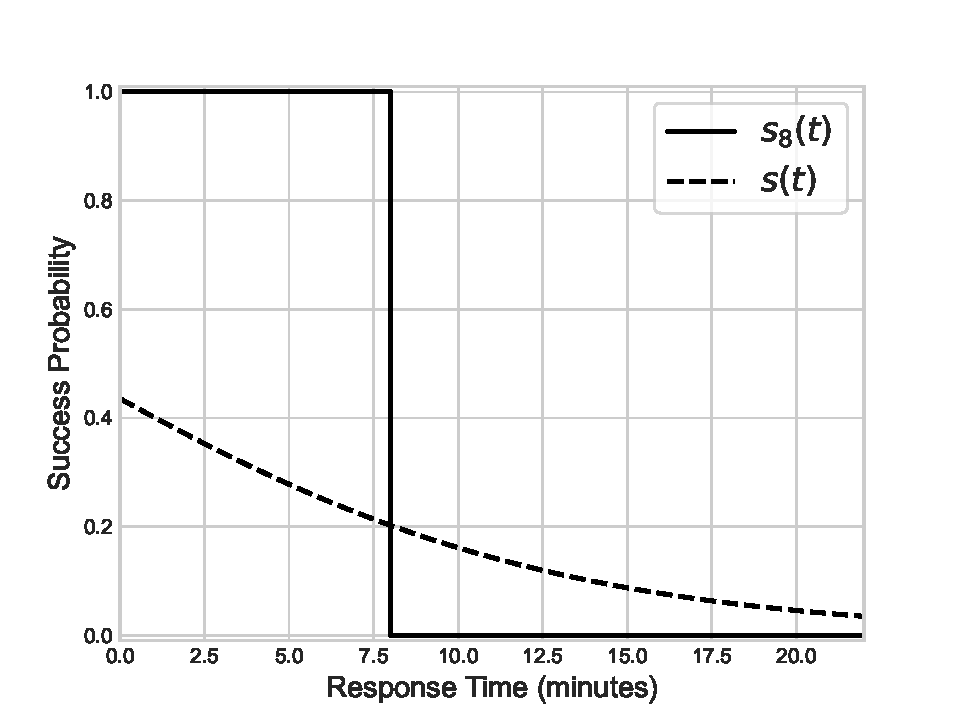
\includegraphics[width=0.5\textwidth]{img/Survival_Function.pdf}
    \caption{Survival function $s(t)$, estimated by \cite{Valenzuela20001206}
             compared with a current EMS target, $s_L(t)$ with $L=8$,
             represented as a step function (binary coverage).}
  \label{fig:survivalfunction}
\end{figure}


\subsection{Maximal Expected Survival Location Model with Heterogeneous
            Patients and Heterogeneous Fleet}\label{sec:meslmhphf}
Here we propose a Maximal Expected Survival Location Model with Heterogeneous
Patients and Heterogeneous Fleet (MESLMHPHF). It is an extension of the
MESLMHP model given in \cite{Knight2012918}, which did not consider
heterogeneous fleets. This is a model of survival that can be used as an
objective function for optimisation algorithms. It is a weighted expected
survival function as the objective function which considers heterogeneous
patients (different specialities) and heterogeneous fleets (both primary
vehicles, EAs, and secondary vehicles, RRVs), and is constructed by
appropriately summing these survival curves, described in
Section~\ref{sec:survival}, across the population, multiplying by ambulance
availability where appropriate.
The MESLMHPHF is given by Equation~\ref{eqn:meslmhphf},

\begin{equation}\label{eqn:meslmhphf}
g\left(Z_a, \tilde{Z}_a\right) =
\sum_{p \in \mathcal{P}} \sum_{a \in \mathcal{A}}
\left( \sum_{k \in \mathcal{K}_A}  w_k \lambda_{pk} \hat{\Psi}_{kpa} +
\sum_{k \in \mathcal{K}_B}  w_k \lambda_{pk} \Psi_{kpa} \right)
\end{equation}

where $w_k$ is a weight associated with patient speciality type $k$ (for this
study we assume $w_k = 1$ for all $k$). Now $\Psi_{kpa}$ can be interpreted as
the probability of a patient $k \in \mathcal{K}_B$ at pick-up location $p$
being seen by a primary vehicle from location $a$ and surviving; while
$\hat{\Psi}_{kpa}$ would be the probability of patients of speciality
$k \in \mathcal{K}_A$ at pick-up location $p$ being seen by any vehicle from
location $a$ and surviving. Equation~\ref{eqn:meslmhphf} is the weighted sum
over the expected survival probabilities of all patient specialities, all
patient pick-up locations, and all ambulance stations. These survival
probabilities are given by Equations~\ref{eqn:survival_A}
and~\ref{eqn:survival_B} respectively,

\begin{equation}\label{eqn:survival_A}
\Psi_{kpa} = s_k\left( b_{pa} \right)
\left(1 - \pi_{a}^{Z_a} \right)
\prod_{\alpha \in \mathcal{A}}
\pi_{\alpha}^{\left(Z_{\alpha} \beta_{p\alpha a} \right)}
\end{equation}

\begin{align}\label{eqn:survival_B}
\hat{\Psi}_{kpa} &= s_k\left(\tilde{b}_{pa}\right)
\left(1 - \tilde{\pi}_{a}^{\tilde{Z}_a} \right)
\prod_{\alpha \in \mathcal{A}}
\tilde{\pi}_{\alpha}^{\left(\tilde{Z}_{\alpha} \beta_{p\alpha a}\right)}
\pi_{\alpha}^{\left(Z_{\alpha} R_{p \alpha a}\right) } \nonumber \\
&+ s_k\left(b_{pa}\right) \left(1 - \pi_{a}^{Z_a} \right)
\prod_{\alpha \in \mathcal{A}}
\pi_{\alpha}^{\left(Z_{\alpha}\beta_{p\alpha a}\right)}
\tilde{\pi}_{\alpha}^{\left(\tilde{Z}_{\alpha}
\left(1 - R _{p a\alpha}\right)\right)}
\end{align}

Here $R_{p a_1 a_2}$ and $\beta_{p a_1 a_2}$ are binary variables indicating
the preference of sending a vehicle from one station to another:
$\beta_{p a_1 a_2}$ indicates if a vehicle of the same type can reach $p$
quicker from $a_1$ than $a_2$, defined in equation~\ref{eqn:beta}, while
$R_{p a_1 a_2}$ indicates if a primary vehicle at $a_1$ can reach $p$ quicker
than a secondary vehicle at $a_2$, defined in equation~\ref{eqn:R}.

\begin{equation}\label{eqn:beta}
\beta_{p a_1 a_2} = \begin{cases}
    0 & \text{if } a_1 = a_2\\
    1 & \text{if } b_{p a_1} \leq b_{p a_2}\\
    0 & \text{otherwise.}
\end{cases}
\end{equation}

\begin{equation}\label{eqn:R}
R_{p a_1 a_2} = \begin{cases}
    1 & \text{if } b_{p a_1} \leq \tilde{b}_{p a_2}\\
    0 & \text{otherwise.}
\end{cases}
\end{equation}

Equation~\ref{eqn:survival_A} is the probability of a patient surviving (their
survival function), multiplied by the availability of primary vehicles at that
ambulance station, multiplied by the unavailability of vehicles at closer
stations.
Equation~\ref{eqn:survival_B} extends this to two vehicles types, the first
part of the sum repeating the logic for the faster secondary vehicles, and the
second part of the sum adapting that logic for primary vehicles, who will only
be contribute the patient's survival if all faster secondary vehicles are also
busy. These interpretations are given as annotations to the equations
in~\ref{apx:annotated}.

A key consideration is the vehicle utilisations $\pi_a$ and $\tilde{\pi}_a$;
discussed in the next subsection.

\subsection{Utilisation Considerations}\label{sec:utilisation}
The models above assume that the utilisations of each vehicle type at each
vehicle location is known, which is a potentially restrictive assumption.
These utilisations $\pi_a$ and $\tilde{\pi}_a$ depend on the demand to station
$a$, which itself depends on the vehicle allocations. One method of overcoming
this, used in \cite{Knight2012918}, is to consider utilisation as the ratio of
demand and service rates, shown in Equations~\ref{eqn:utilisation_ratio_primary}
and~\ref{eqn:utilisation_ratio_secondary}. Here we let $\frac{1}{\mu}$ and
$\frac{1}{\tilde{\mu}}$ be the average job times of primary and secondary
vehicles, then $\lambda_a$ and $\tilde{\lambda}_a$ represent the share of the
demand seen by primary and secondary vehicles from vehicle location $a$,
respectively.

\begin{align}
\pi_a &= \frac{\lambda_a}{\mu} \label{eqn:utilisation_ratio_primary}\\
\tilde{\pi}_a &= \frac{\tilde{\lambda_a}}{\tilde{\mu}} \label{eqn:utilisation_ratio_secondary}
\end{align}

Note that here we assume that average job times are not dependant on the vehicle
location $a$, although this may be unrealistic, given that the travel between
locations are a key part of an vehicle's job time ($B_{pa}$, $D_{ya}$, $F_{pa}$).
However, as discussed in Section~\ref{sec:problem_description}, there are a
number of other components to an ambulance job including time on site ($G_k$),
hospital handover time ($J_{yk}$), and vehicle refill time ($\Theta$). We
justify the assumption of job times not being location dependant by considering
the proportion of an ambulance job's time that is location dependant, $\rho$,
defined in Equation~\ref{eqn:proportion_location_dependant}.

\begin{equation}\label{eqn:proportion_location_dependant}
\rho = \begin{cases}
  \frac{B_{pa} + D_{ya}}{T_{paky}} & \text{ if hospital required,} \\[8pt]
  \frac{B_{pa} + F_{pa}}{T_{pak}} & \text{ if no hospital required.}
\end{cases}
\end{equation}

Then, using the simulation described later in Section~\ref{sec:simulation}, we
consider the distribution of $\rho$ across all simulated jobs under the current
situation and allocation in Jakarta, shown in Figure~\ref{fig:rho_distribution}.
We see for primary vehicle jobs on average 24\% of a job time is location
dependant, while it is 36.5\% for secondary vehicles. Therefore this assumption
should not have too much of an effect for primary vehicles, whose job times are
much longer than secondary vehicles, but leaves open questions about how to
better handle this assumption for secondary vehicles.

\begin{figure}
    \centering
    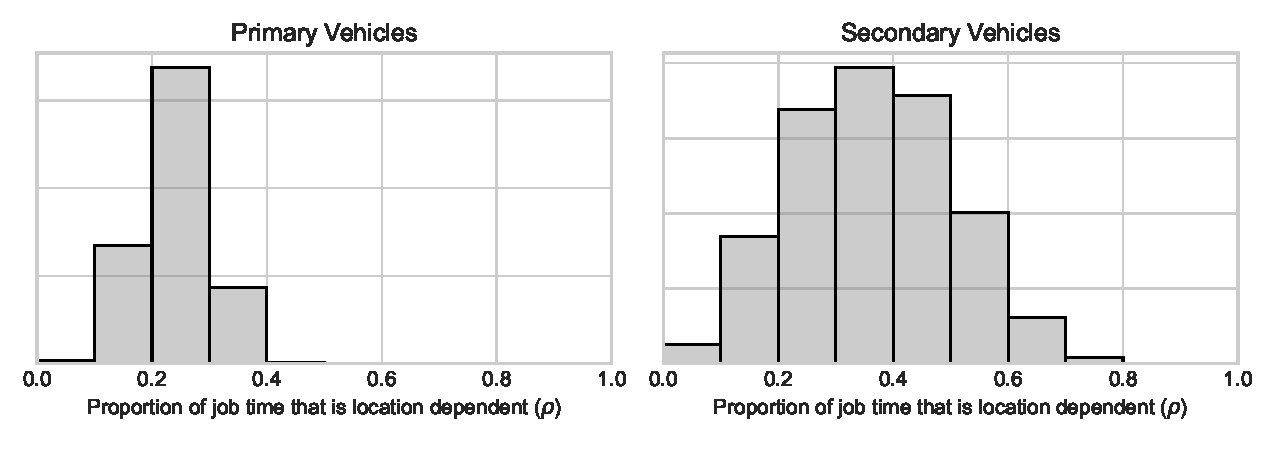
\includegraphics[width=0.85\textwidth]{img/location_dependant_service_time_proportion}
    \caption{Distribution of the proportion of an ambulance job consists of
    location dependant components, for primary and secondary vehicles.}
    \label{fig:rho_distribution}
\end{figure}

On the other hand, the demand experienced by vehicles at each location
$a \in \mathcal{A}$ would be location specific, and would depend on the number
and utilisation of the vehicles at every other location.


\subsection{Numerical approximation of utilisation}
For primary vehicles, which operate independently of secondary vehicles, the
relationship between demand experienced at each location, $\lambda_a$, and the
allocations and utilisations of all other locations, is given by
Equation~\ref{eqn:utilisations_primary}. For secondary vehicles, the
relationship between demand experienced at each location, $\tilde{\lambda}_a$,
and the allocations and utilisations of all other locations, is given by
Equation~\ref{eqn:utilisations_primary}. Note that this also depends on the
utilisations of the primary vehicles, $\pi_a$.

\begin{equation}\label{eqn:utilisations_primary}
\lambda_a = \sum_{p \in \mathcal{P}} \sum_{k \in \mathcal{K}} \lambda_{pk}
\left( 1 - \left(\frac{\lambda_a}{\mu}\right)^{Z_a} \right)
\prod_{\alpha \in \mathcal{A}} \left(\frac{\lambda_{\alpha}}{\mu}\right)^{
\left(Z_{\alpha} \beta_{p \alpha a}\right)}
\end{equation}

\begin{equation}\label{eqn:utilisations_secondary}
\tilde{\lambda}_a = \sum_{p \in \mathcal{P}}
\sum_{k \in \mathcal{K}_A} \lambda_{pk}
\left( 1 - \left(\frac{\tilde{\lambda}_a}{\tilde{\mu}}\right)^{\tilde{Z}_a} \right)
\prod_{\alpha \in \mathcal{A}} \pi_{\alpha}^{\left(Z_{\alpha} R_{p \alpha a}\right)}
\left(\frac{\tilde{\lambda}_{\alpha}}{\tilde{\mu}}\right)^{
\left(\tilde{Z}_{\alpha} \beta_{p \alpha a}\right)}
\end{equation}

We propose finding the true vehicle utilisations by first solving
Equation~\ref{eqn:utilisations_primary} for the $\lambda_a$; determining the
primary vehicle utilisations with Equation~\ref{eqn:utilisation_ratio_primary};
then using these to solve Equation~\ref{eqn:utilisations_secondary} for the
$\tilde{\lambda}_a$; and determining the secondary vehicle utilisations with
Equation~\ref{eqn:utilisation_ratio_secondary}. These can be solved
numerically. In our implementation this is solved using the MINPACK hybrd and
hybrj algorithms by using Scipy's \texttt{fsolve} function
\cite{2020SciPy-NMeth}.




\subsection{Heuristic Optimisation}\label{sec:heuristic}
In order to maximise the MESLMHPHF objective function presented in
Section~\ref{sec:meslmhphf}, we use a population-based neighbourhood search
evolutionary heuristic algorithm. A population of possible solutions is
created and ranked according to the objective, then for each generation of the
heuristic a proportion of the best performing solutions is kept, and are
mutated to complete the population for the next generation. To encourage
exploration, the number of times each solution is mutated begins high and
gradually decreases throughout the run of the simulation.
The heuristic takes five hyper-parameters: $N$ the population size, $\kappa$
the number of solutions to retain to the next generation, $m_0$ the initial
mutation rate; $c$ the cooling rate; and $H$ the number of generations. The
heuristic is described in Algorithm~\ref{alg:heuristic}.

\begin{algorithm}
\SetAlgoLined
Create a population of $N$ random allocations ($Z_a$, $\tilde{Z}_a$)\;
\For{$i \leftarrow 0$ \KwTo $H$}{
  Rank the population according to Equation~\ref{eqn:meslmhphf}\;
  Keep the top $\kappa$ solutions\;
  $m \leftarrow \lceil m_0 - \max\left(m_0, i c\right)\rceil$\;
  \For{$j \leftarrow 0$ \KwTo $N - \kappa$}{
    Randomly choose and copy a solution from the population\;
    Mutate that copy of the solution $m$ times\;
    Place mutated copy in a separate population\;
  }
  Combine populations;\
}
Rank the population according to Equation~\ref{eqn:meslmhphf};\
Output the top ranking solution.
\caption{Population-based Neighbourhood Search Evolutionary Algorithm}
\label{alg:heuristic}
\end{algorithm}

Mutations one of four possible changes: randomly change the location of one
primary vehicle; randomly change the location of one secondary vehicle;
randomly remove one primary vehicle and add secondary vehicles to 3 randomly
chosen locations; and randomly remove 3 secondary vehicles and add a primary
vehicle to a randomly chosen location. If it is required that exact vehicle
numbers need to be retained, then only for first two mutations need be chosen.

The source code for the optimisation heuristic, including the evaluation of
the MESLMHPHF objective function and the solution method for the utilisation
considerations, is given in
\url{https://github.com/drvinceknight/upgraded-octo-barnacle}.
Numerical results are discussed in Section~\ref{sec:jakarta}.




\section{Simulating Allocations}\label{sec:simulation}
Discrete event simulation (DES) is a common methodology that allows us to
investigate given scenarios under uncertainty. Here it will be used to
quantify the effectiveness of given ambulance allocations by measuring a range
of key performance indicators (KPIs), such as the average response time, the
percentage of abandoned calls, vehicle utilisations, and expected survival
based on response times. The simulation is built using the Ciw library
\cite{palmer2019ciw}, and the model logic is described below. Its central
ideas include modelling transit jobs as customers, rather than the patients
themselves, and simulating primary and secondary vehicles as two simulations
sequentially, with the output of the former being the input of the latter.


\subsection{Simulating Primary Vehicles}\label{sec:simulation_primary}
For primary vehicles the logic to simulate is as follows: Patients make a call
from one of a number of pick-up locations and await an ambulance to pick them
up and take them to an appropriate hospital. Ambulances are stationed at a
number of ambulance locations; when a patient makes a call, all free
ambulances from any location calculate their expected time to reach that
patient, and the ambulance with the smallest expected time to the patient is
called out. The ambulance drives from its current ambulance location to the
patient's pick-up location, then if a hospital is required, from the patient's
pick-up location to the hospital, and then from the nearest hospital back to
their original ambulance location. If a hospital is not required, the
ambulance returns to their original ambulance location.

Rather than considering patients as customers in a queue, here the situation
is re-framed to model transit jobs as customers, with the ambulances as
servers.

Transit jobs can be categorised into classes corresponding to the pick-up
locations $\mathcal{P}$ and speciality $\mathcal{K}$. Jobs of class
$(p, k) \in \mathcal{P} \times \mathcal{K}$ arrive with rate $\lambda_{pk}$.
Servers can be categorised into classes corresponding to the ambulance
locations $\mathcal{A}$. Service times are server-dependent, that is the
service time of a transit job of type $(p, k)$, being served by a server of
class $a$, will have service time $T_{paky}$ if a hospital is required and
$T_{pak}$ if no hospital is required. These are given by
Equations~\ref{eqn:service_time_withhosp} and~\ref{eqn:service_time_nohosp}
respectively, in Section~\ref{sec:problem_description}.
That is $T_{paky}$ and $T_{pak}$ is the overall time the ambulance spends
dealing with that transit job and is unavailable to receive any more transit
jobs.

From a patient's point of view their service only lasts $G_k + C_{py} + J_{yk}$,
(or $G_k$ if no hospital is required), and their waiting time is $B_{pa}$ plus
the time waiting for an ambulance to be dispatched. However in our case, if
there are no free ambulances at the time of call, it is assumed that patients
find their own care or transport, and so the call is abandoned. Therefore, the
time waiting for dispatch is always zero.

Furthermore, all service times are time dependent, and calculated from travel
distances and approximate hourly traffic levels, described in
Section~\ref{sec:travel_times}.

\subsection{Travel Time Calculations}\label{sec:travel_times}
Each day is split into a set of periods, $\mathcal{H}$ indexed by $h$. Within
each period traffic levels are considered constant but differ from period to
period. Traffic levels influence the speed of the ambulance through a delay
factor $d_h$ associated with each period. Therefore, the expected speed $S_h$
at which an ambulance travels during period $h$ is given by
Equation~\ref{eqn:speed},

\begin{equation}\label{eqn:speed}
S_h = s d_h
\end{equation}

where $s$ is some given baseline speed. The relationship between time travelled
and distance covered is piece-wise linear with slope $S_h$ in period $h$.
Therefore, travel times are calculated using this relationship.

As an example, consider the scenario where for the first period $t \in (0, 4)$
we have $S_1$ = 1; for $t \in (4, 8)$ we have $S_2 = \frac{1}{4}$, for
$t \in (8, 12)$ we have $S_3 = 2$, and for $t \in (12, 16)$ we have $S_4 = 1$.
Consider that the vehicle must travel 11 units. If the vehicle begins its
journey at $t=0$, then the expected travel time would be 11 time units, shown
in Figure~\ref{fig:travel_times_1}. However if the vehicle begins its journey
at time $t=3$ then the expected travel time is 10 time units, shown in
Figure~\ref{fig:travel_times_2}.

\begin{figure}
    \begin{center}
    \begin{subfigure}{6.6cm}
    \includestandalone[scale=0.33]{img/travel_times}
    \caption{Beginning at $t=0$, a travel time of $11$.}
    \label{fig:travel_times_1}
    \end{subfigure}
    \begin{subfigure}{6.6cm}
    \includestandalone[scale=0.33]{img/travel_times_2}
    \caption{Beginning at $t=3$, a travel time of $10$.}
    \label{fig:travel_times_2}
    \end{subfigure}
    \end{center}
    \caption{Example of calculating travel times for two different starting
    times.}
    \label{fig:travel_times}
\end{figure}

This is the method used to calculate the expected values of $B_{pa}$, $C_{py}$,
$D_{ya}$ and $F_{pa}$.
Furthermore it is assumed that travel times for each segment of the route
(from vehicle location to patient, from patient to hospital, and from hospital
back the the vehicle's location) follow a Triangular distribution around the
calculated expected travel time, between 75\% and 125\% of the value.


\subsection{Time-dependent Demand}
Additionally, it is assumed that calls arrive according to a Poisson
distribution, with rates $\lambda{pk}$, and that these rates are time
dependent. Each day is split into four 6-hour periods, the morning, afternoon,
evening and night, and each speciality $k$ and pick-up location $p$ will have
a different call arrival rate for each of these periods.

For some locations and specialities the number of observed calls might be very
low, and so the $\lambda{pk}$ rate would be very low. This can cause
synchronicity issues when sampling arrivals \citep{pidd2004computer}, where
artificially long inter-arrival times can be introduced at the beginning of
one time period due to the low arrival rate in the previous time period.
In order to overcome this here, rather than sample inter-arrival times
iteratively from an Exponential distribution, an entire schedule of arrival
dates are sampled at the beginning of the simulation run, first by sampling
the number of arrivals required in each time period from a Poisson
distribution, and then by sampling specific dates within that time period
using a Uniform distribution.

This mechanism, and alternative to thinning \cite{lewisshedler79}, was
implemented in the Ciw software in version v2.3.3 \cite{ciw233}, and described
in the documentation here:
\url{https://ciw.readthedocs.io/en/latest/Guides/time_dependent.html}.


\subsection{Simulating Secondary Vehicles}\label{sec:simulation_secondary}
Secondary non-transit vehicles, can in general travel faster than primary
transport vehicles, and so can be dispatched at the same time as a primary
vehicle but reach the patient earlier, reducing the response time for that
patient and thus their survival probability. They are only dispatched for
patients of speciality $k \in \mathcal{K}_A$, and if the closest secondary
vehicle can reach them before the closest primary vehicle.
Here secondary vehicles are simulated in a second discrete event simulation,
run sequentially, but simulating the exact same time period and events as the
first simulation. This is similar to sequential hybrid simulation methodology
\cite{brailsfordetal19, morganetal17}, however in this case the two combined
components are both DES, and are combined to simplify the logic of each
component.

This is possible as there are no synchronicity issues between the two
components. Primary vehicles operate independently of secondary vehicles, that
is the way primary vehicles respond to a patient is unaffected by the presence
or lack of a secondary vehicle.
Therefore, primary vehicle logic is not compromised by simulating primary
vehicles in isolation.
Secondary vehicles are impacted by the behaviour of primary vehicles, they
must remain with the patient until the primary vehicle arrives, and so must be
simulated after the simulation of primary vehicles, taking as inputs the exact
list of events that occurred. That is the logic of the secondary vehicles is
determined by observing the actions of primary vehicles and reacting to them.
Simulation results are combined for each individual patient, to determine
their response time caused by either primary or secondary vehicles.

Secondary vehicles are chosen in the same way was primary vehicles, by choosing
out of the currently free vehicles the one with the smallest expected time to
patient. Their service times are reactionary to what occurred with the primary
vehicle.
Let $\tilde{B}_{pa_2}$ be the time it takes for the secondary vehicle to travel
from its location $a_2$ to the patient pick-up location $p$; $B_{pa_1}$ is the
time is took for the primary vehicle to get from its location $a_1$ to the
patient pick-up location $p$; $G_k$ is the time the primary vehicle spent
with the patient; and $\tilde{F}_{pa_2}$ is the time is takes to return to the
secondary vehicle's location $a_2$ from the patient pick-up location $p$.
Note that $B_{pa_1}$ and $G_k$ are exact values obtained from the
initial simulation of the primary vehicles, while $\tilde{B}_{pa_2}$ and
$\tilde{F}_{pa_2}$ are random variables to sample in the subsequent simulation.
Travel times are calculated as described in Section~\ref{sec:travel_times},
replacing the primary vehicle delay factor, $d_h$, with a delay factor for
secondary vehicles, $\tilde{d}_h$. This accounts for secondary vehicles
travelling faster and reacting to traffic differently to primary vehicles.

Exact synchronicity considerations are shown in Figure~\ref{fig:sequential_logic}:
\begin{itemize}
  \item whenever the secondary vehicle reaches the patient before the primary
  vehicle, they remain with the patient until the primary vehicle leaves;
  \item if secondary vehicle arrives after the primary vehicle they will
  immediately return to their stations as they are not needed at the scene;
  \item if the expected time for the secondary vehicle to reach the patient
  exceeds the expected time for the primary vehicle to reach the patient then
  the secondary vehicle is not deployed, and so that transit job would be
  abandoned in the secondary simulation (although still seen by a primary
  vehicle in the initial simulation).
\end{itemize}

Therefore job service times for secondary vehicles, $\tilde{T}_{pak}$, are
given by:

\begin{equation}
  \tilde{T}_{pak} = \max\left(\tilde{B}_{pa_2}, B_{pa_1} + G_k \right) + \tilde{F}_{pa_2}
\end{equation}

\begin{figure}
    \centering
    \includestandalone[scale=0.6]{img/synchronicity}
    \caption{Visualising secondary vehicle (SV) logic reacting to the primary
    vehicle's (PV) actions.}
    \label{fig:sequential_logic}
\end{figure}

\subsection{Combined Model}
Combining the logic presented in Sections~\ref{sec:simulation_primary}
and~\ref{sec:simulation_secondary} gives the overall simulation logic for
simulating both primary and secondary vehicle types. It is used to quantify
the effectiveness of a given allocation $(Z_a, \tilde{Z}_a)$ for all
$a \in \mathcal{A}$, by recording several useful KPIs.
In this work, the KPIs of interest are: the average primary vehicle
utilisation, the average secondary vehicle utilisation, the mean response
time, the percentage of abandoned calls (that is a measure of the primary
vehicle unavailability), and the expected overall survival. Survival is
modelled using a combination of survival function curves and hard cut-offs,
and is described in Section~\ref{sec:survival}.



\section{The Case of Jakarta}\label{sec:jakarta}
Jakarta, the capital of Indonesia, has a population of 10.5 million
\cite{BPS_Jakarta} residing within 664 km$^2$. The city is divided into five
municipalities and one district, each of which is divided into sub districts
and, in turn, neighbourhoods. There is a total of 42 sub districts and 261
neighbourhoods within mainland Jakarta (excluding the Thousand Islands regency
in the north) \cite{BPS_Jakarta_angka}, a map is given in
Figure~\ref{fig:region_names}. 

As described in Section~\ref{sec:intro}, there are many challenges to calling
for an ambulance in Jakarta, as captured in \cite{BriceSyaribahNoor2022Esui}.
This work showed and initially fragmented ambulance service with poor data
collection meaning that estimating the true demand for ambulances in Jakarta
was itself particularly challenging.
Based on this work the regional government of Jakarta invested in a new fleet
of coordinated ambulances accessible via the single emergency number 119.
This work, in collaboration with Ambulans 118 and the 119 Emergency Ambulance
Service, finds potential fleet allocations using the optimisations methods
given in Section~\ref{sec:optimising}, and evaluates these allocations'
effectiveness using the simulation described in Section~\ref{sec:simulation}.

\begin{figure}
\begin{center}
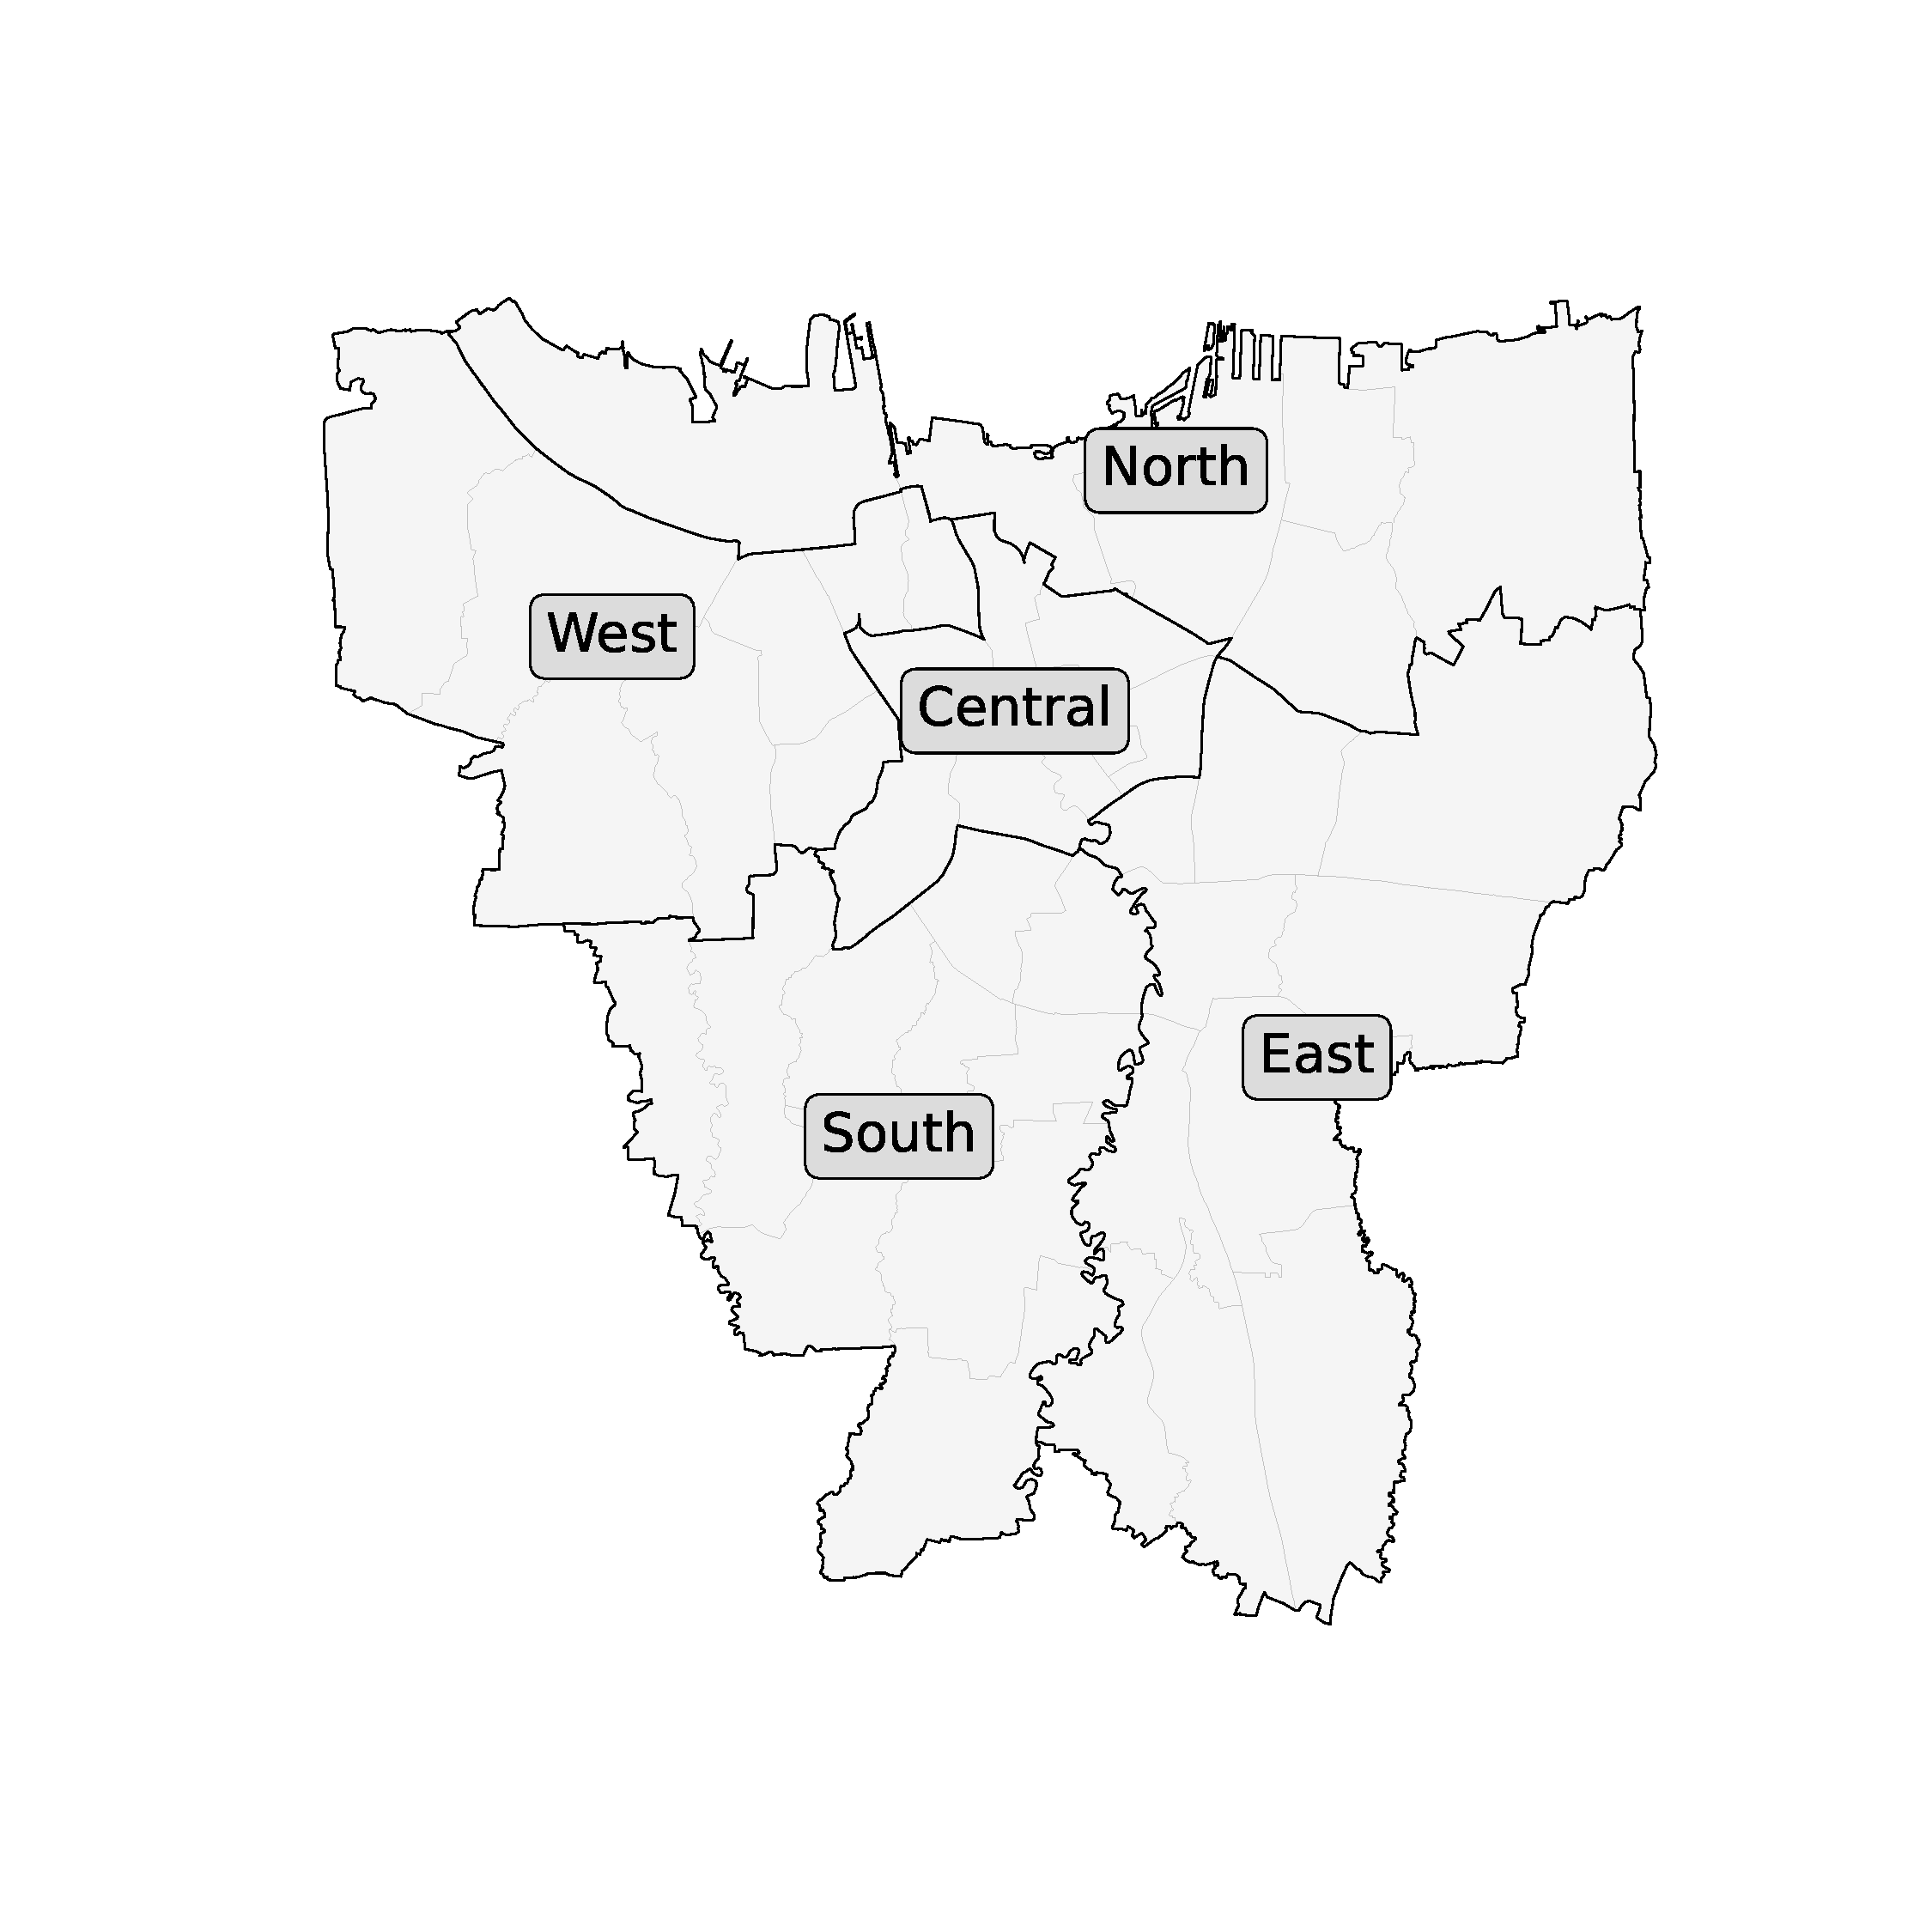
\includegraphics[width=0.55\textwidth,trim={0 6cm 0 5cm}, clip]{img/jakarta_region_names.pdf}
\end{center}
\caption{Map of Jakarta's Municipalities.}
\label{fig:region_names}
\end{figure}

As of October 2022, the 119 service in Jakarta ran a fleet of 81 primary
Emergency Ambulances (EAs) and 13 secondary motorbike Rapid Response Vehicles
(RRVs), distributed across 67 ambulance stations throughout the city.
Figure~\ref{fig:current_allocation} summarise the allocations vehicle
locations.

\begin{figure}
\begin{center}
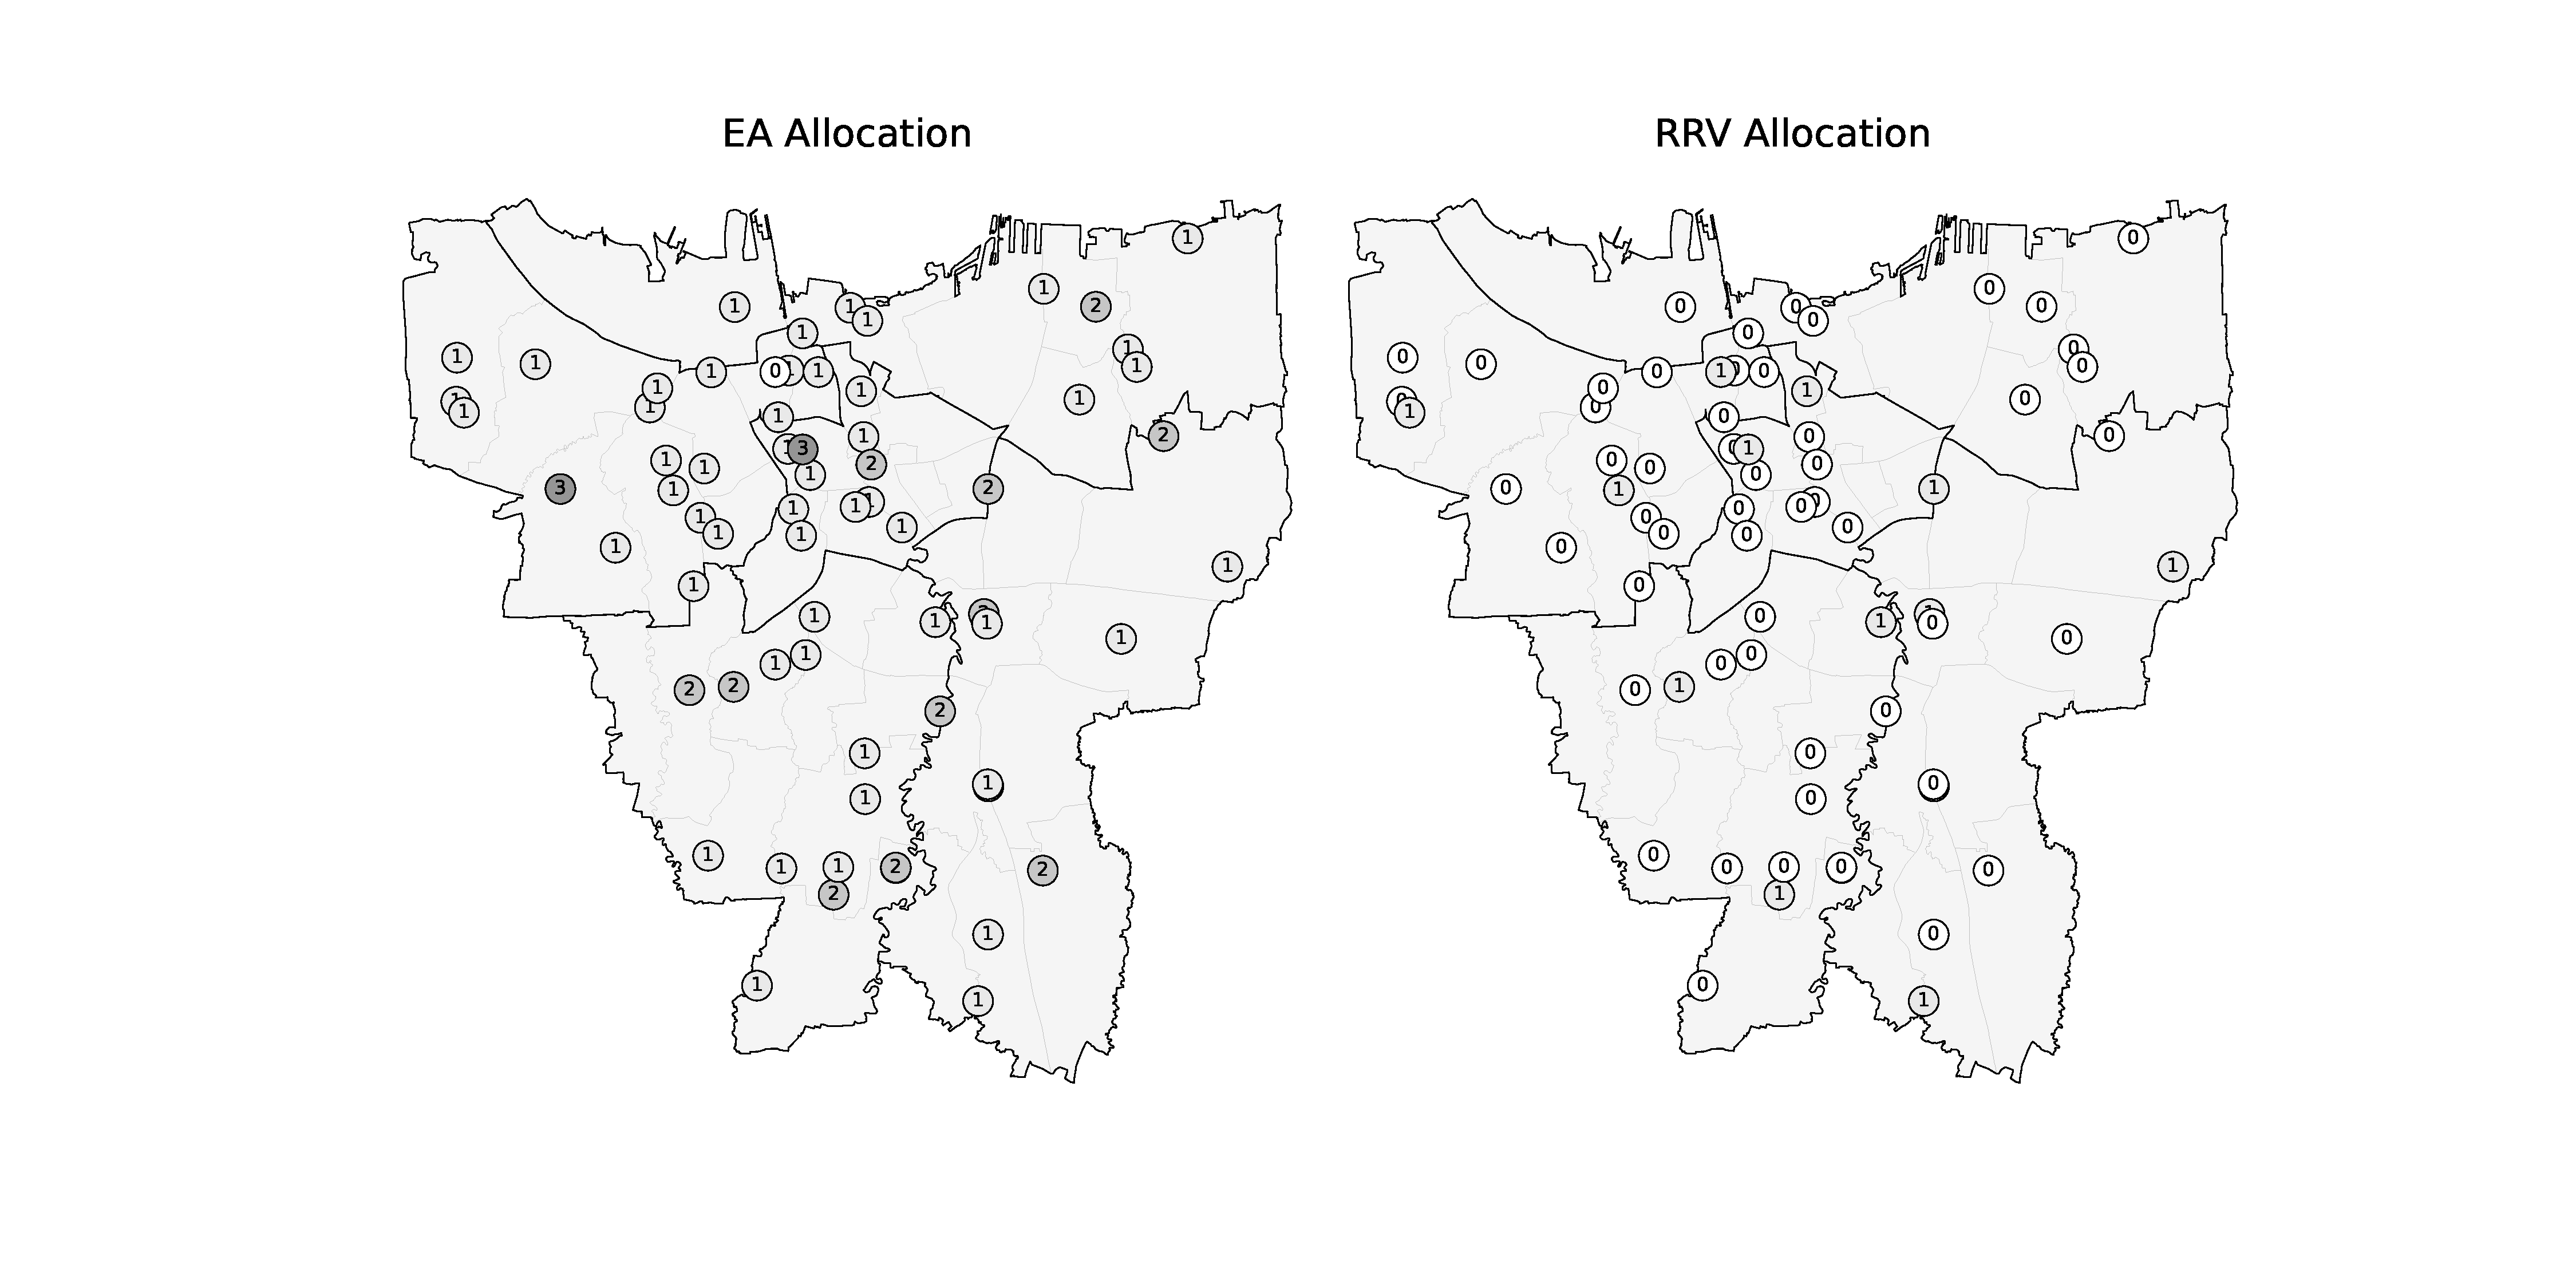
\includegraphics[width=\textwidth]{img/map_current}
\caption{Map of current Emergency Ambulance (EA) and Rapid Response Vehicle
         (RRV) locations and allocations to ambulance bases across Jakarta.}
\label{fig:current_allocation}
\end{center}
\end{figure}

Working with our ambulance partners, after careful consideration the following
patient `specialities' ($k \in \mathcal{K}$) were agreed based on clinical need
(although other categories could readily be adopted and included as necessary):

\begin{itemize}
  \item \textbf{A1 - High priority emergency patients}: critical patients who
  require immediate life-saving assistance with a target ambulance response
  time of 8 minutes. In our data set there were 168 identified calls that met
  this criterion.
  \item \textbf{A2 - Other emergency patients}: urgent patients that require
  assistance with a target response time of 15 minutes. In our data set there
  were 23,784 calls of this type.
  \item \textbf{B - Non-emergency patients}: patients that still benefit from
  an ambulance response but non-critical with a target response time of 60
  minutes. There were 31,725 calls of this type in the data set.
\end{itemize}

Here secondary vehicles can be called to patients of speciality A1 and A2,
therefore $\mathcal{K}_A = \{\text{A1}, \text{A2}\}$ and
$\mathcal{K}_B = \{\text{B}\}$.
The number of calls from each of these specialities varies by neighbourhood,
as shown in Figure~\ref{fig:yearly_demand}. It can be seen that many calls are
highly concentrated in a handful of neighbourhoods rather than spread
throughout the city.

\begin{figure}
\begin{center}
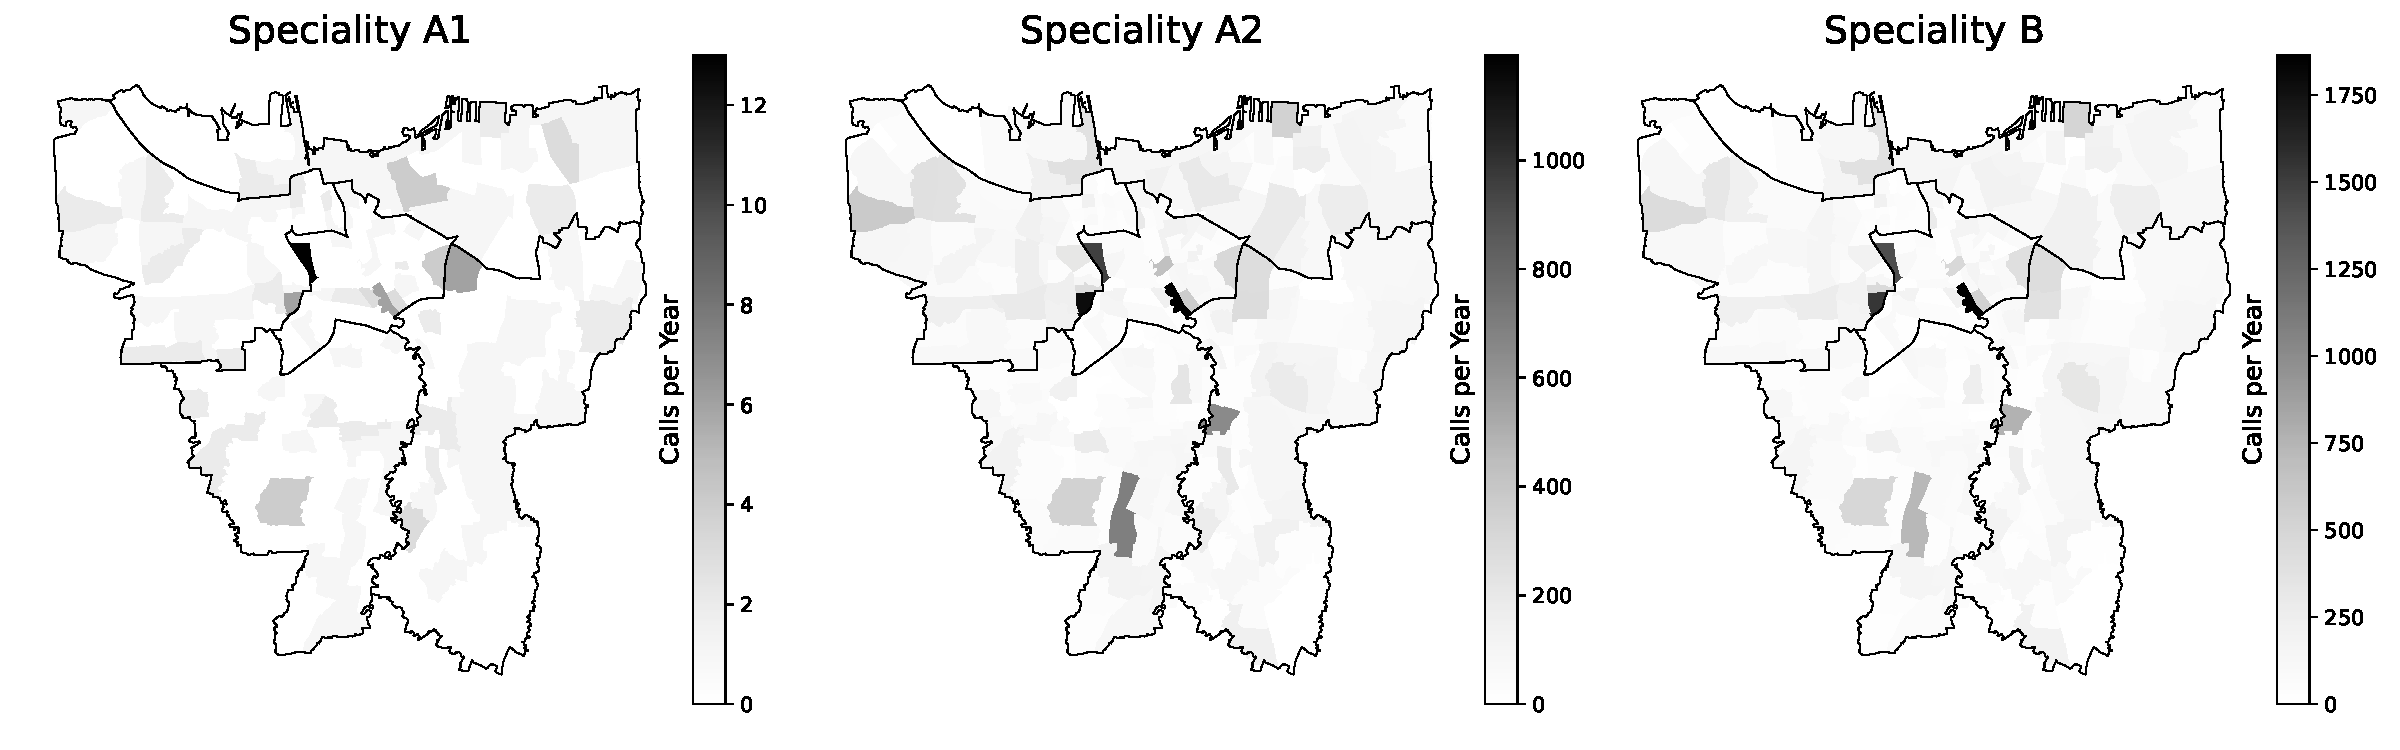
\includegraphics[width=\textwidth]{img/yearly_demand.pdf}
\end{center}
\caption{Number of calls received by speciality and neighbourhood.}
\label{fig:yearly_demand}
\end{figure}


Firstly, in Section~\ref{sec:analysis_grid} we use the MESLMHPHF objective
function of expected survival, and the simulation, to find KPIs that to compare
the performance of two proposed grid allocations to the currently used
allocation. Then in Section~\ref{sec:demand_scenarios} we outline four possible
future demand scenarios, and in Section~\ref{sec:optimise_current} we use the
optimisation model to find and compare optimised allocations for the current
number of vehicles. Finally in Section~\ref{sec:vehicle_numbers} we investigate
the number of vehicles required to meet the demand across the given scenarios.

All models are parameterised using demand data that covers all 261
neighbourhoods from 1 January to 31 December 2019, before the COVID-19
pandemic. Data from 2020-2021 was naturally heavily skewed by the pandemic,
with significantly lower demand, and so was not considered as representative
of a typical period for forecasting future needs, hence the decision to use
the available 2019 demand. \ref{apx:parameters} provides further details on the
parameterisation of the model.


\subsection{Evaluating `Grid' Proposals}\label{sec:analysis_grid}
The 119 Discussions with senior staff at 119 identified that they were seriously
considering to re-configure their ambulance allocations into a grid structure,
placing an ambulance station at regular intervals throughout the city and
uniformly distributing the vehicles that they felt would ensure coverage. Two
possible grid allocations were being considered: one placing an EA every 3km
across the city (giving a total of 70 vehicles), and another placing three EAs
every 5km across the city (giving a total of 72 vehicles).
Figure~\ref{fig:grid_allocations} show these proposed allocations.

\begin{figure}
\begin{center}
\begin{subfigure}{0.48\textwidth}
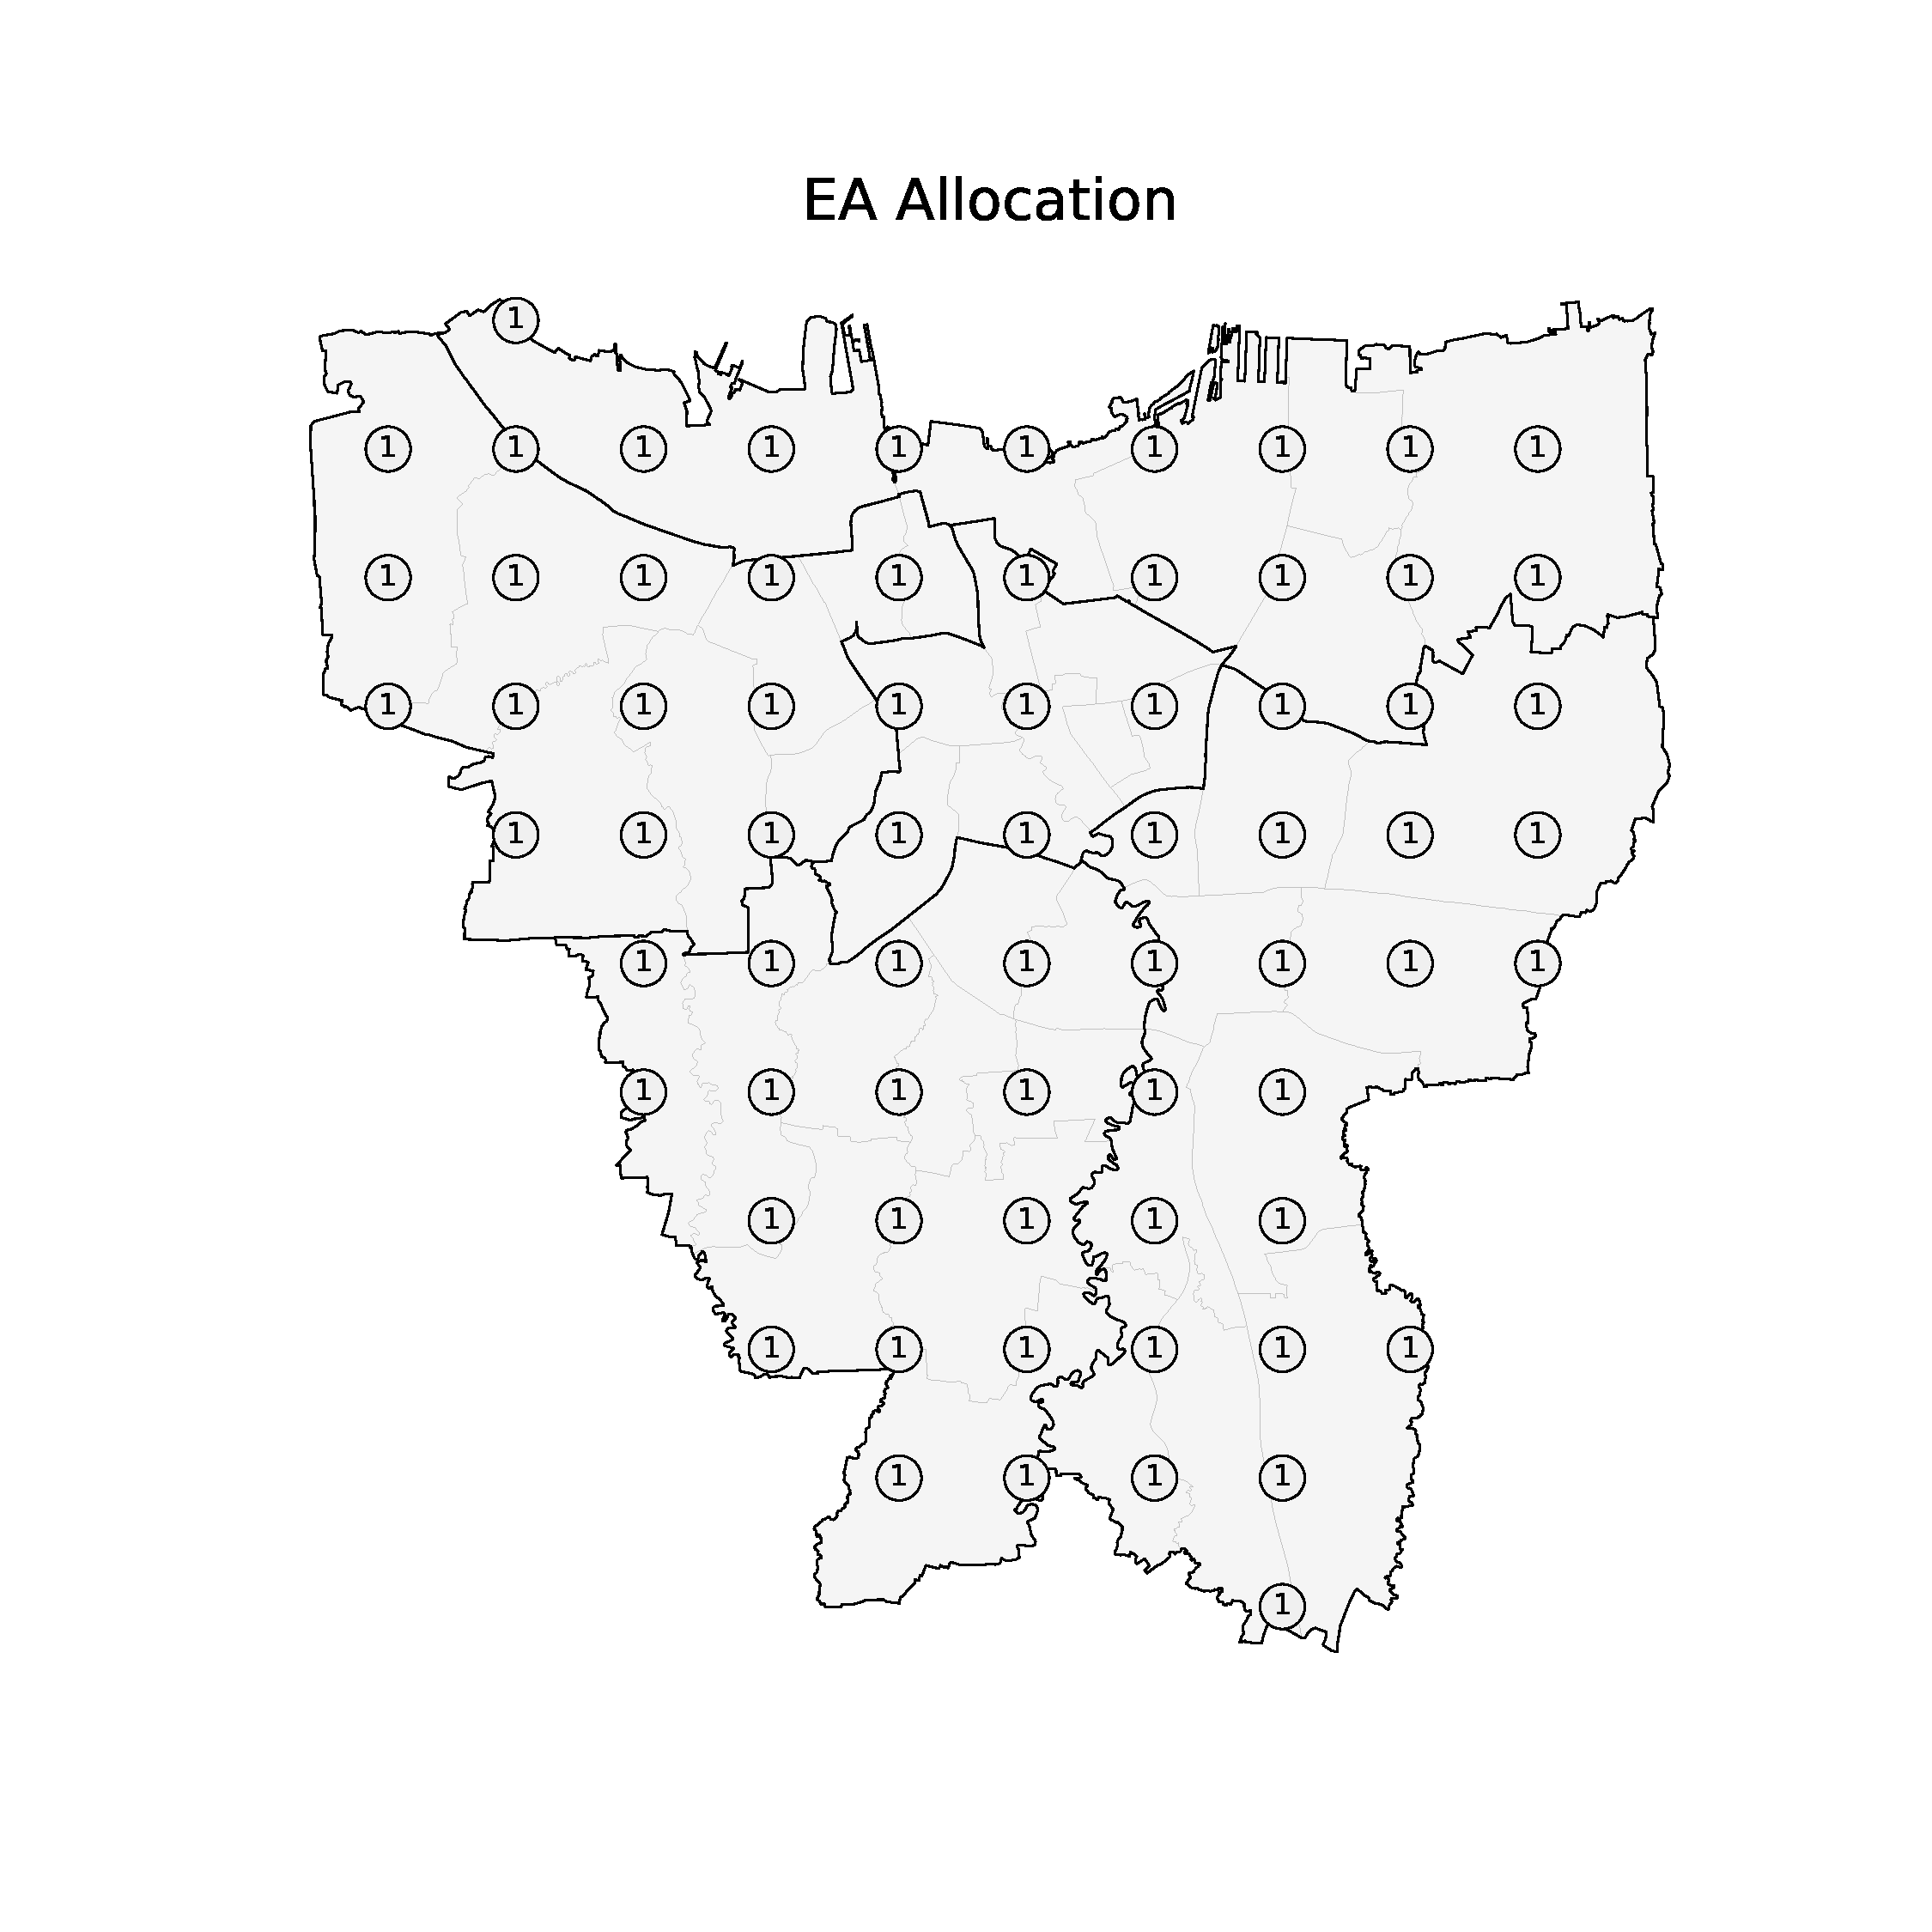
\includegraphics[width=\textwidth]{img/map_grid3km_proposed}
\caption{3km grid.}
\end{subfigure}
\hfill
\begin{subfigure}{0.48\textwidth}
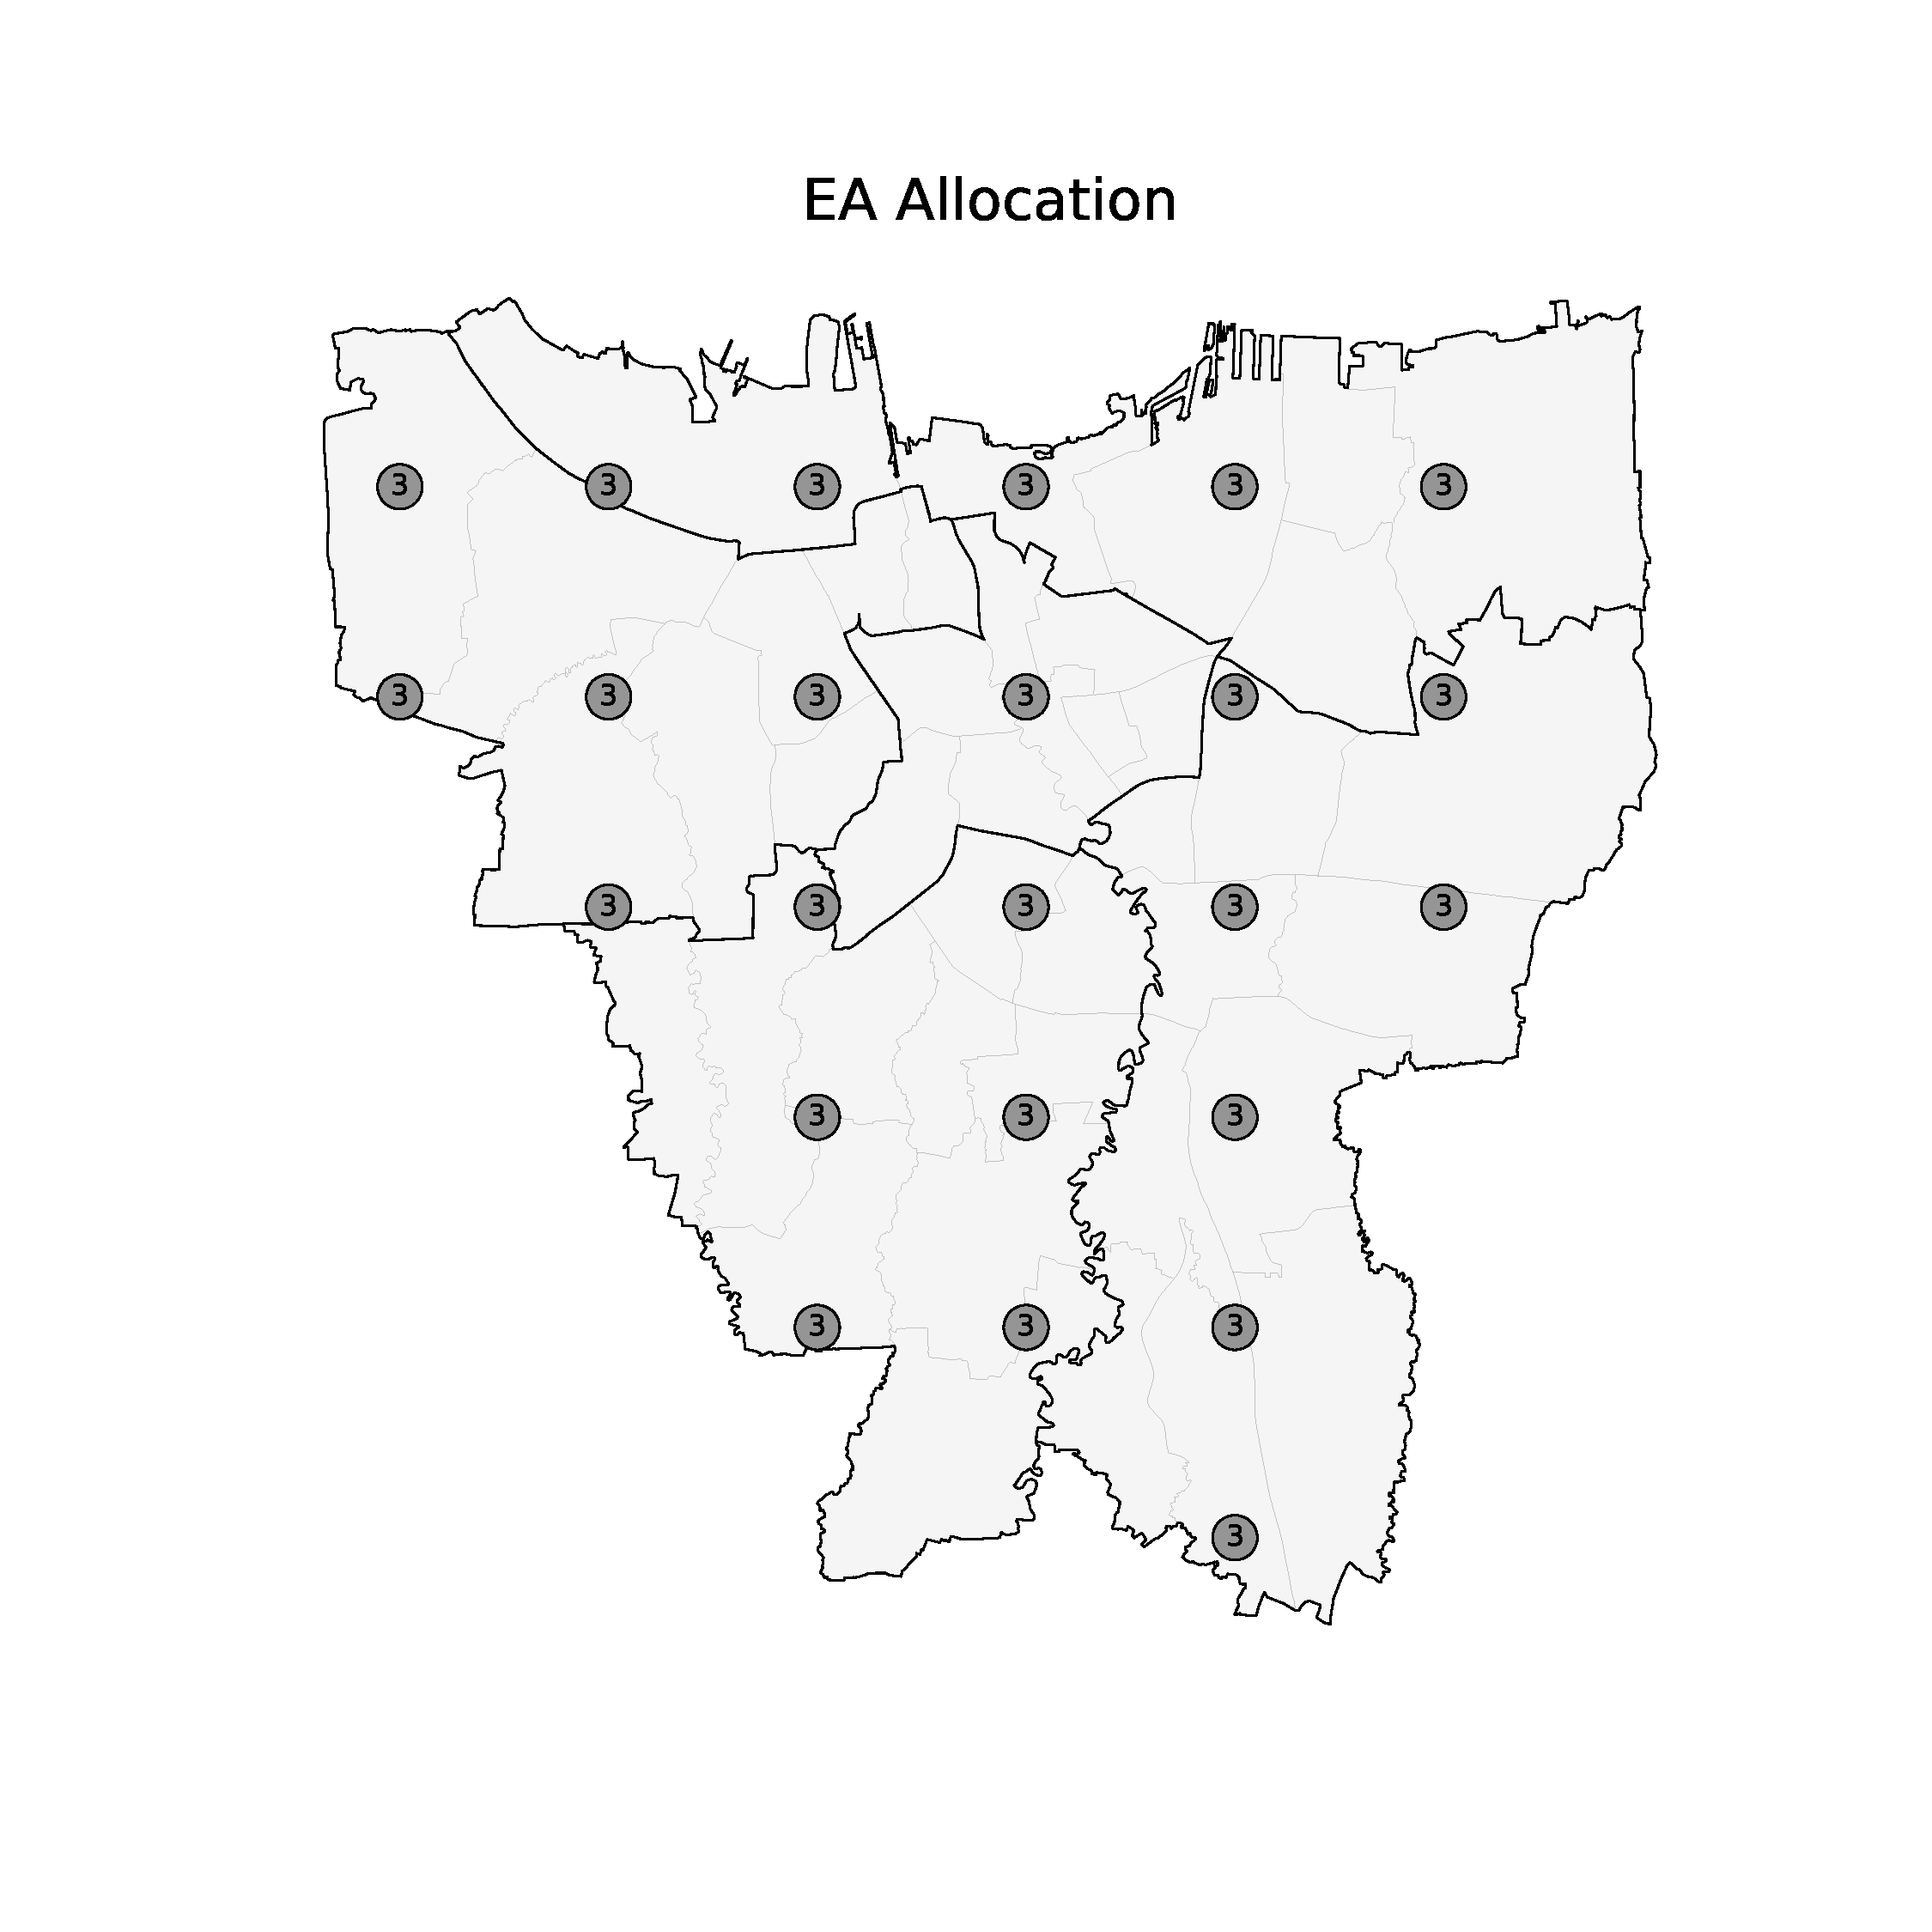
\includegraphics[width=\textwidth]{img/map_grid5km_proposed}
\caption{5km grid.}
\end{subfigure}
\caption{Proposed grid allocations.}
\label{fig:grid_allocations}
\end{center}
\end{figure}

Running the simulation and MESLMHPHF objective function of expected survival for
both the current and the two proposed grid allocations gives the results shown
in Table~\ref{tbl:current_grid_results}. We observe that the two proposed
grid allocations perform much worse than the current allocation as measured by
mean response time, survival, and percentage of calls abandoned.
This is expected as vehicle numbers are lower under the new proposals, as well
as the allocations focussing on coverage rather than response times or survival.

\begin{table}
\begin{center}
\begin{tabular}{rrrr}
\toprule
Allocation & Baseline & Grid 3km & Grid 5km \\
\midrule
Number of EAs & 81 & 70 & 71 \\
Number of RRVs & 13 & 0 & 0 \\
Ambulance Utilisation & 31.7\% & 37.4\% & 36.6\% \\
RRV Utilisation & 40.9\% & - & - \\
Mean Response Time (mins) & 16.80 & 22.39 & 24.14 \\
Overall Survival & 75.5\% & 63.7\% & 61.0\% \\
Percent Abandoned & 0.034\% & 0.430\% & 1.028\% \\
\bottomrule
\end{tabular}
\caption{Calculated KPIs for the current and proposed grid allocations.}
\label{tbl:current_grid_results}
\end{center}
\end{table}


\subsection{Planning for Future Demand}\label{sec:demand_scenarios}
Similarly to many other cities worldwide, ambulance services in Jakarta
anticipate that demand for services will grow in future years, not least that
there is now a coordinated service accessible via a single common number `119'
to call. This should help raise awareness and visibility of an ambulance
service. In the case of Jakarta, certainly increased use of 119 and therefore
increased demand would be a desired outcome resulting from proactive actions
by the Indonesian Government. 

We consider four different demand scenarios, developed by considering the
result of our cross-sectional study of patients attending EDs in Jakarta
\cite{BriceSyaribahNoor2022Esui}. As part of the survey, randomly selected
patients arriving at each emergency department were asked whether they had
used an ambulance to attend, and reasons for not using an ambulance. For those
patients who were categorised by the medical staff as emergency and for whom
therefore an ambulance might have seemed a sensible option, the responses are
given in Table~\ref{table:survey_results}.

\begin{table}
\centering
\begin{tabular}{rr}
\toprule
Reason & \% of emergency respondents \\
\midrule
Used Ambulance & 13.0\\
Too expensive & 5.2  \\
Not available  & 13.1 \\
Would take too long & 16.5 \\
Not necessary & 15.7  \\
Not aware of service & 33.1\\
Other &3.5 \\
\bottomrule
\end{tabular}
\caption{Barriers to use of an ambulance service in Jakarta, from
         \cite{BriceSyaribahNoor2022Esui}.}
\label{table:survey_results}
\end{table}

The survey confirmed three major barriers to use, namely: the service's
visibility (33.1\% of respondents were unaware of the service), the service's
reliability (13.1\% of respondents reported that there was no ambulance
available and 16.5\% of respondents believed it would take too long), and the
service's cost (5.2\% of respondents cited cost as a deterrent). Therefore,
four demand scenarios were considered, corresponding to addressing each of
these barriers in turn:

\begin{itemize}
  \item \textbf{D13}: representing the current situation where approximately
        13\% of emergency patients (specialities A1 and A2) do use an ambulance.
  \item \textbf{D19}: representing the situation where visibility is addressed.
        Here, we distribute the 33.1\% of the respondents who were unaware of
        the service proportionally between using the ambulance and amongst the
        remaining issues. Using this methodology we would expect 19.4\% of
        emergency patients to now use an ambulance.  
  \item \textbf{D34}: representing the situation where reliability and
        visibility are addressed. Using the same methodology we would expect
        34.8\% of emergency patients to now use an ambulance.
  \item \textbf{D45}: representing the situation where cost, reliability and
        visibility are all addressed. Using the same methodology we would expect
        45.4\% of emergency patients to now use an ambulance. 
\end{itemize}

Guided by our findings in \cite{BriceSyaribahNoor2022Esui}, recent changes
mean that the 119 services is now free to use for Jakarta residents, so
certainly the highest demand (demand\_45) scenario is plausible in the near
future. After discussions with our partners, it was agreed that for each of
the scenarios we should assume that non-emergency demand (speciality B)
remains unchanged.


\subsection{Improving the Current Allocation}\label{sec:optimise_current}
Applying the optimisation heuristic from Section~\ref{sec:optimising} to the
current allocation re-allocates the 81 EAs and 13 RRVs. We do this for each of
the four scenarios described in Section~\ref{sec:demand_scenarios}. The
hyper-parameters used for this optimisation algorithm throughout this study are
given in Table~\ref{tbl:hyperparameters}, which include approximations for the
average service times of primary and secondary vehicles derived from the initial
simulation model. \ref{apx:hyperparameters} shows some initial explorations on
the hyperparameter choices, giving confidence that the chosen parameters, with
a large enough number of iterations $N$, are sufficient to find allocations
that perform well.

\begin{table}
\begin{tabular}{lll}
\toprule
Parameter & Value Used & Explanation \\
\midrule
$\mu$ & $\frac{1}{3.886 \times 60}$ & Average primary vehicle service rate.\\
$\tilde{\mu}$ & $\frac{1}{1.038 \times 60}$ & Average secondary vehicle service rate.\\
$N$ & 240 & Population size.\\
$\kappa$ & 40 & Number of solutions to keep per generation.\\
$m_0$ & 6 & Initial number of mutations.\\
$c$ & 0.25 & Cooling rate, rate at which number of mutations decreases.\\
$H$ & 500 & Number of generations.\\
\bottomrule
\end{tabular}
\caption{Hyper-parameters used in the optimisation for all experiments.}
\label{tbl:hyperparameters}
\end{table}

Table~\ref{tbl:current_optimal_compare} compares the MESLMHPHF objective
function value and simulation derived KPIs between the current and the optimised
allocations, for each demand scenario. It can be seen that a number of them
increase.

\begin{table}
\begin{center}
\resizebox{\textwidth}{!}{%
\begin{tabular}{lrrrrrr}
\toprule
Demand & Allocation & \specialcellr{Expected\\Survival} & \specialcellr{Primary\\Utilisation} & \specialcellr{Secondary\\Utilisation} & \specialcellr{Mean Response\\Time (mins)} & Abandoned \\
\midrule
\multirow{2}{*}{\textbf{D13}} & Current   & 98.34\% & 28.30\% & 20.43\% & 17.67 & 0.00\% \\
                              & Optimised & 99.10\% & 28.37\% & 16.67\% & 17.83 & 0.00\% \\
\midrule
\multirow{2}{*}{\textbf{D19}} & Current   & 97.74\% & 34.70\% & 29.38\% & 18.44 & 0.43\% \\
                              & Optimised & 99.64\% & 34.71\% & 24.74\% & 18.46 & 0.44\% \\
\midrule
\multirow{2}{*}{\textbf{D34}} & Current   & 95.78\% & 49.49\% & 47.85\% & 22.18 & 3.45\% \\
                              & Optimised & 99.61\% & 49.55\% & 44.82\% & 22.10 & 3.79\% \\
\midrule
\multirow{2}{*}{\textbf{D45}} & Current   & 92.88\% & 56.63\% & 55.80\% & 24.02 & 9.70\% \\
                              & Optimised & 99.54\% & 56.49\% & 52.04\% & 23.19 & 9.29\% \\
\bottomrule
\end{tabular}%
}
\caption{Calculated KPIs for the current and optimised allocations under the
four possible demand scenarios.}
\label{tbl:current_optimal_compare}
\end{center}
\end{table}


\subsection{Finding Optimal Allocations for Any Resource Level}\label{sec:vehicle_numbers}
The heuristic algorithm described in Section~\ref{sec:heuristic} finds
allocation of ambulances across the 67 current ambulance stations for a given
number of primary and secondary vehicles. Information supplied by one of the
ambulance operators suggested that in terms of total running costs one EA
(primary vehicle) was approximately equivalent to three RRVs (secondary
vehicles), and so we consider three RRVs to be one resource; that is, a
resource level of 60 could represent 60 primary and 0 secondary vehicles, or
59 primary and 3 secondary vehicles, or 58 primary and 6 secondary vehicles,
and so on. For a given resource level we run the optimisation algorithm for
all possible combinations of numbers of primary and secondary vehicles, though
as every patient must be seen by a primary vehicle, we do not consider the
case when the number of secondary vehicles exceeds the number of primary
vehicles.
Allocations were found for each resource level between 60 and 125 EA
equivalents, and we report KPIs for the best performing, in terms of maximal
survival, combinations, as well as for the case when the number of secondary
vehicles is fixed at zero. We call these the multiple vehicle type and single
vehicle type scenarios.

Figures~\ref{fig:results_ambulance_utilisation}-\ref{fig:results_overall_survival}
display the obtained KPIs for each of these allocations. It can immediately be
seen that increasing the resource level has a positive effect on all KPIs,
with vehicle utilisations, mean response times, and percentage abandoned
decreasing, and overall survival increasing. Similarly, as expected increasing
the demand of emergency calls has a negative impact on all KPIs.

\begin{figure}
\begin{center}
\begin{subfigure}{0.48\textwidth}
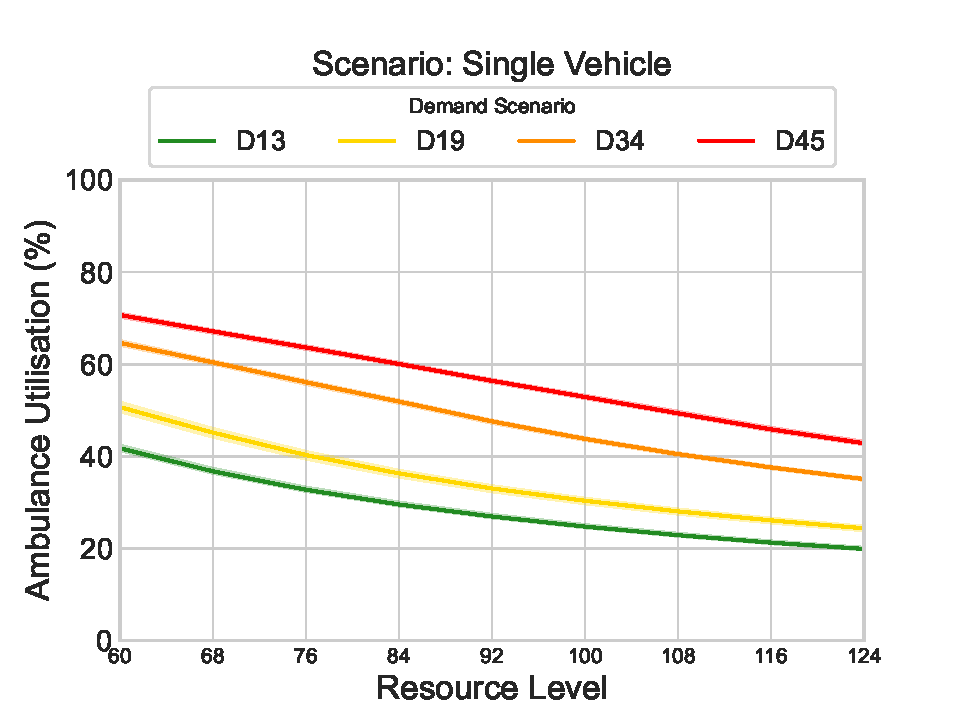
\includegraphics[width=\textwidth]{img/results/single_AmbulanceUtilisation}
\caption{Single vehicle type scenario.}
\label{fig:results_ambulance_utilisation_single}
\end{subfigure}
\begin{subfigure}{0.48\textwidth}
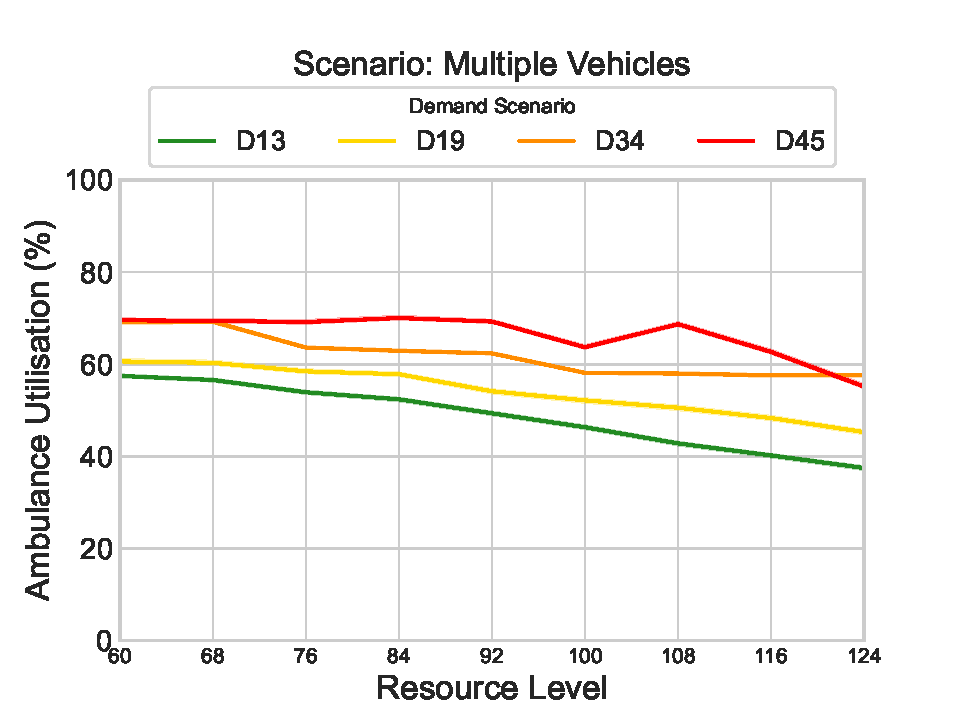
\includegraphics[width=\textwidth]{img/results/multiple_AmbulanceUtilisation}
\caption{Multiple vehicle type scenario.}
\label{fig:results_ambulance_utilisation_multiple}
\end{subfigure}
\end{center}
\caption{Ambulance utilisation results.}
\label{fig:results_ambulance_utilisation}
\end{figure}

\begin{figure}
\begin{center}
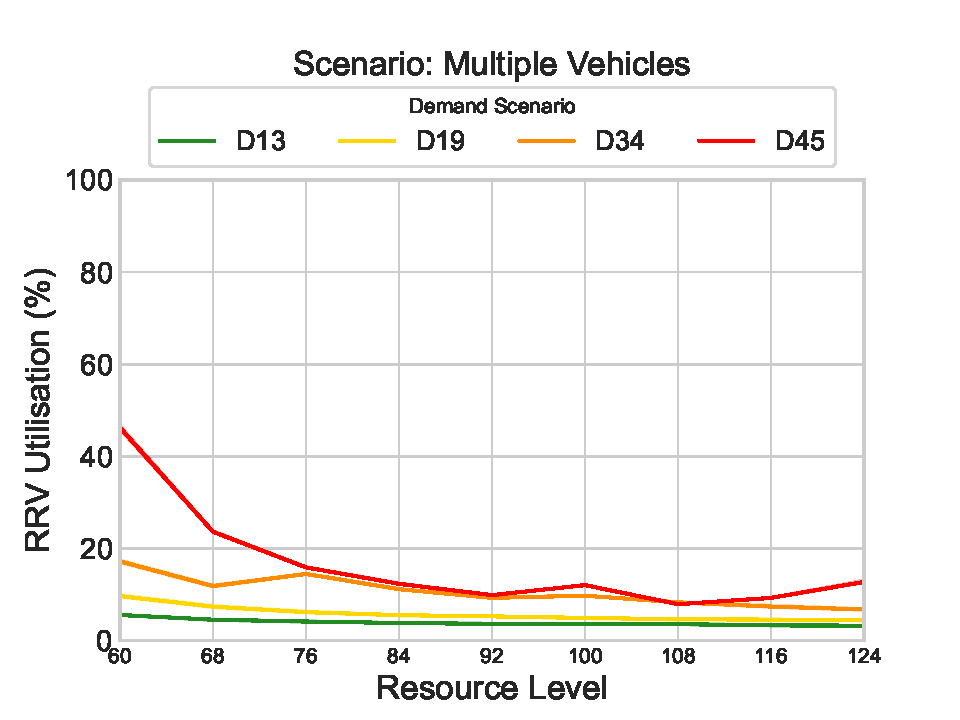
\includegraphics[width=0.48\textwidth]{img/results/multiple_RRVUtilisation}
\end{center}
\caption{RRV utilisation results.}
\label{fig:results_rrv_utilisation_multiple}
\end{figure}

\begin{figure}
\begin{center}
\begin{subfigure}{0.48\textwidth}
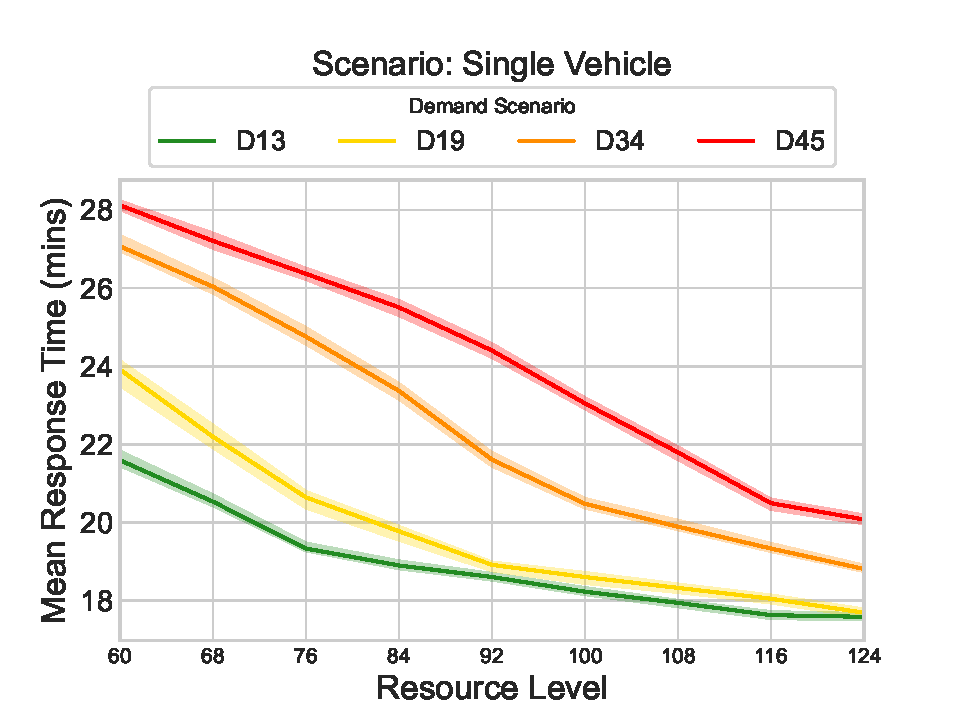
\includegraphics[width=\textwidth]{img/results/single_MeanResponseTime}
\caption{Single vehicle type scenario.}
\label{fig:results_response_single}
\end{subfigure}
\begin{subfigure}{0.48\textwidth}
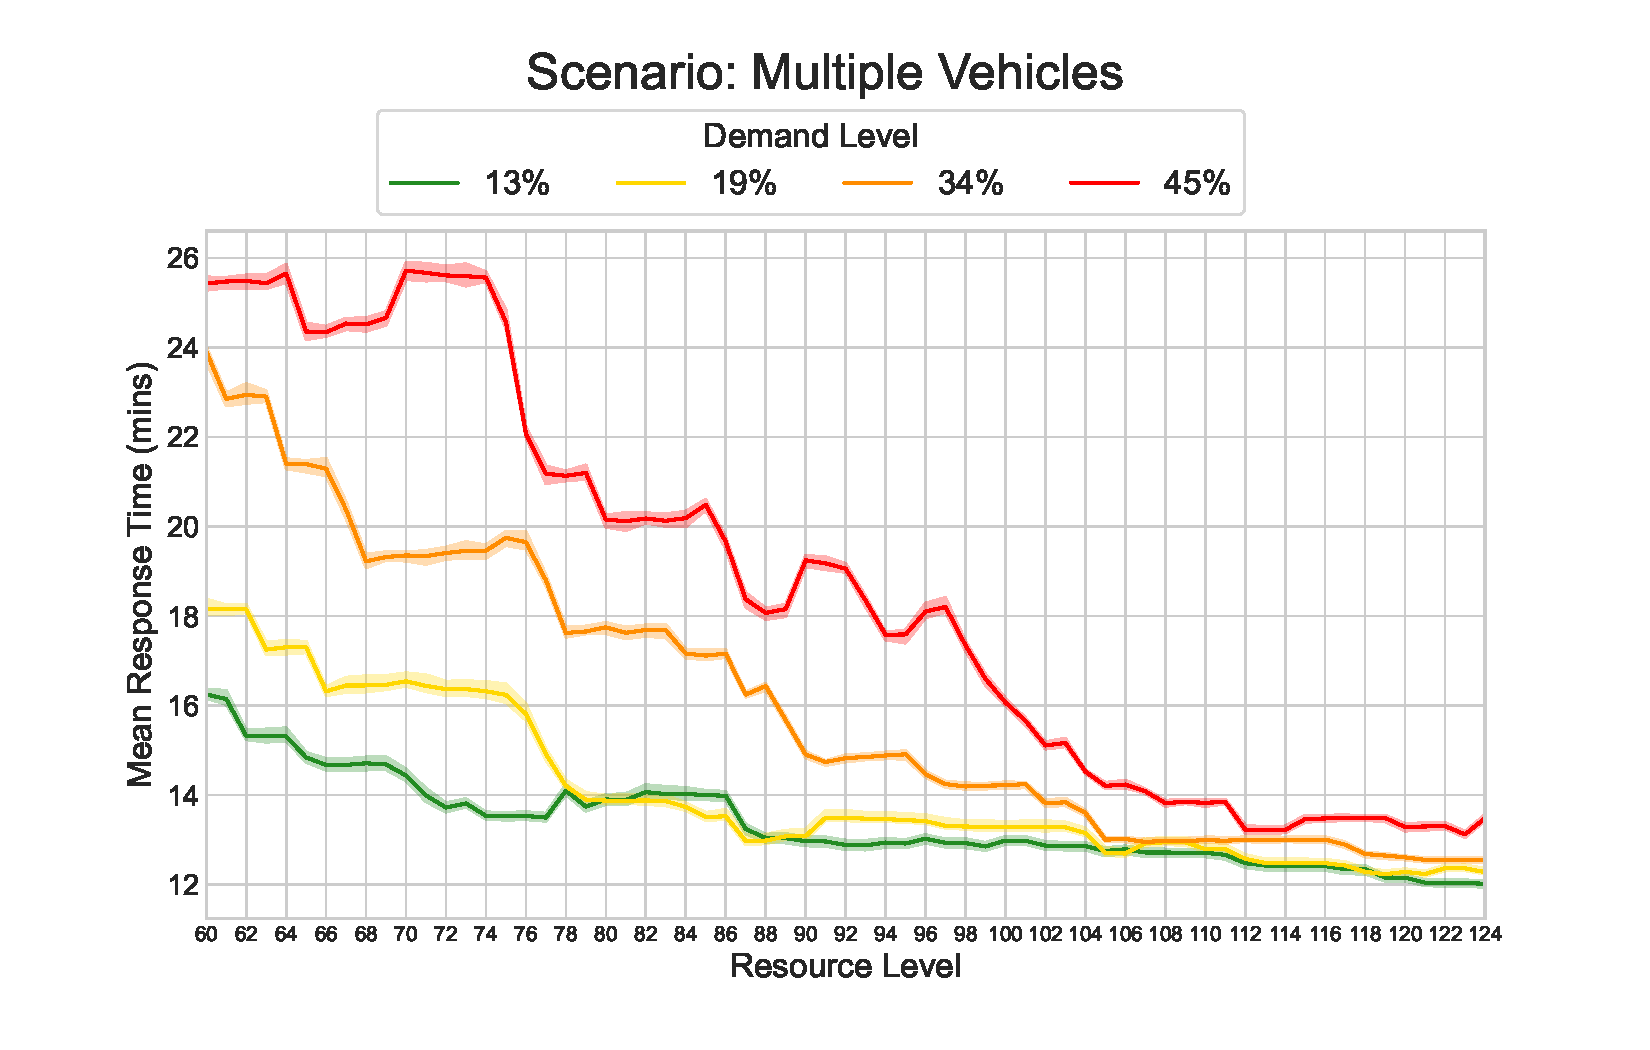
\includegraphics[width=\textwidth]{img/results/multiple_MeanResponseTime}
\caption{Multiple vehicle type scenario.}
\label{fig:results_response_multiple}
\end{subfigure}
\end{center}
\caption{Mean response time results.}
\end{figure}

\begin{figure}
\begin{center}
\begin{subfigure}{0.48\textwidth}
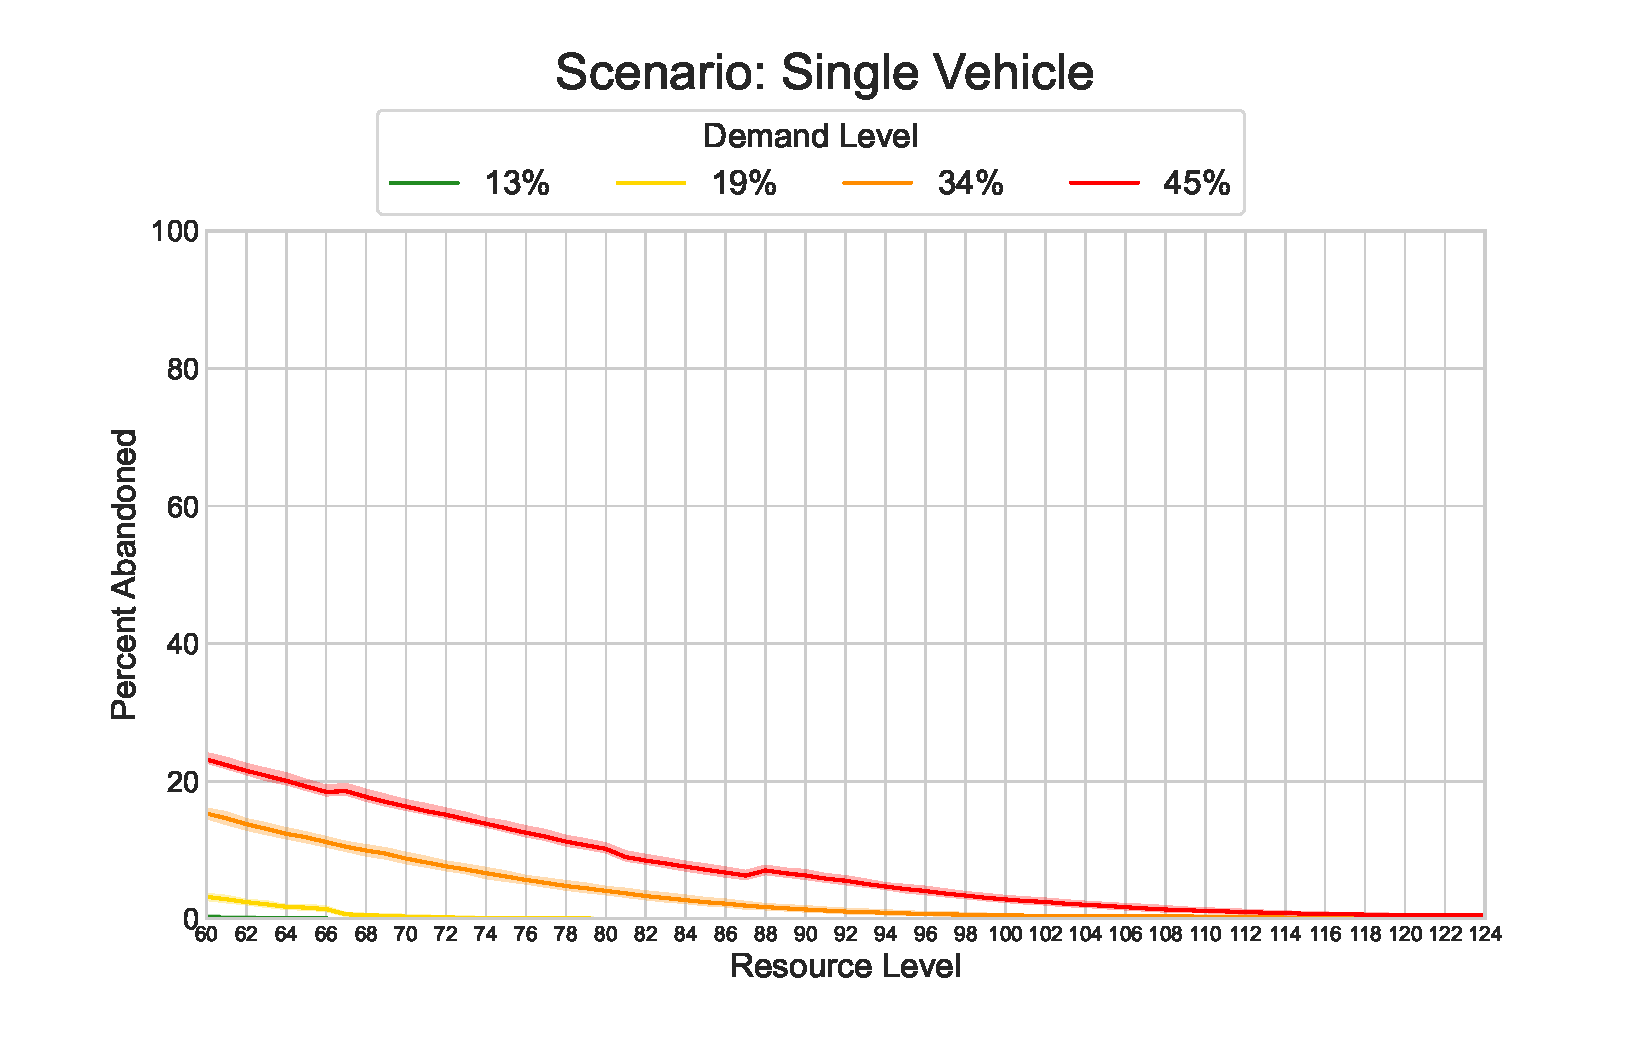
\includegraphics[width=\textwidth]{img/results/single_PercentAbandoned}
\caption{Single vehicle type scenario.}
\label{fig:results_abandoned_single}
\end{subfigure}
\begin{subfigure}{0.48\textwidth}
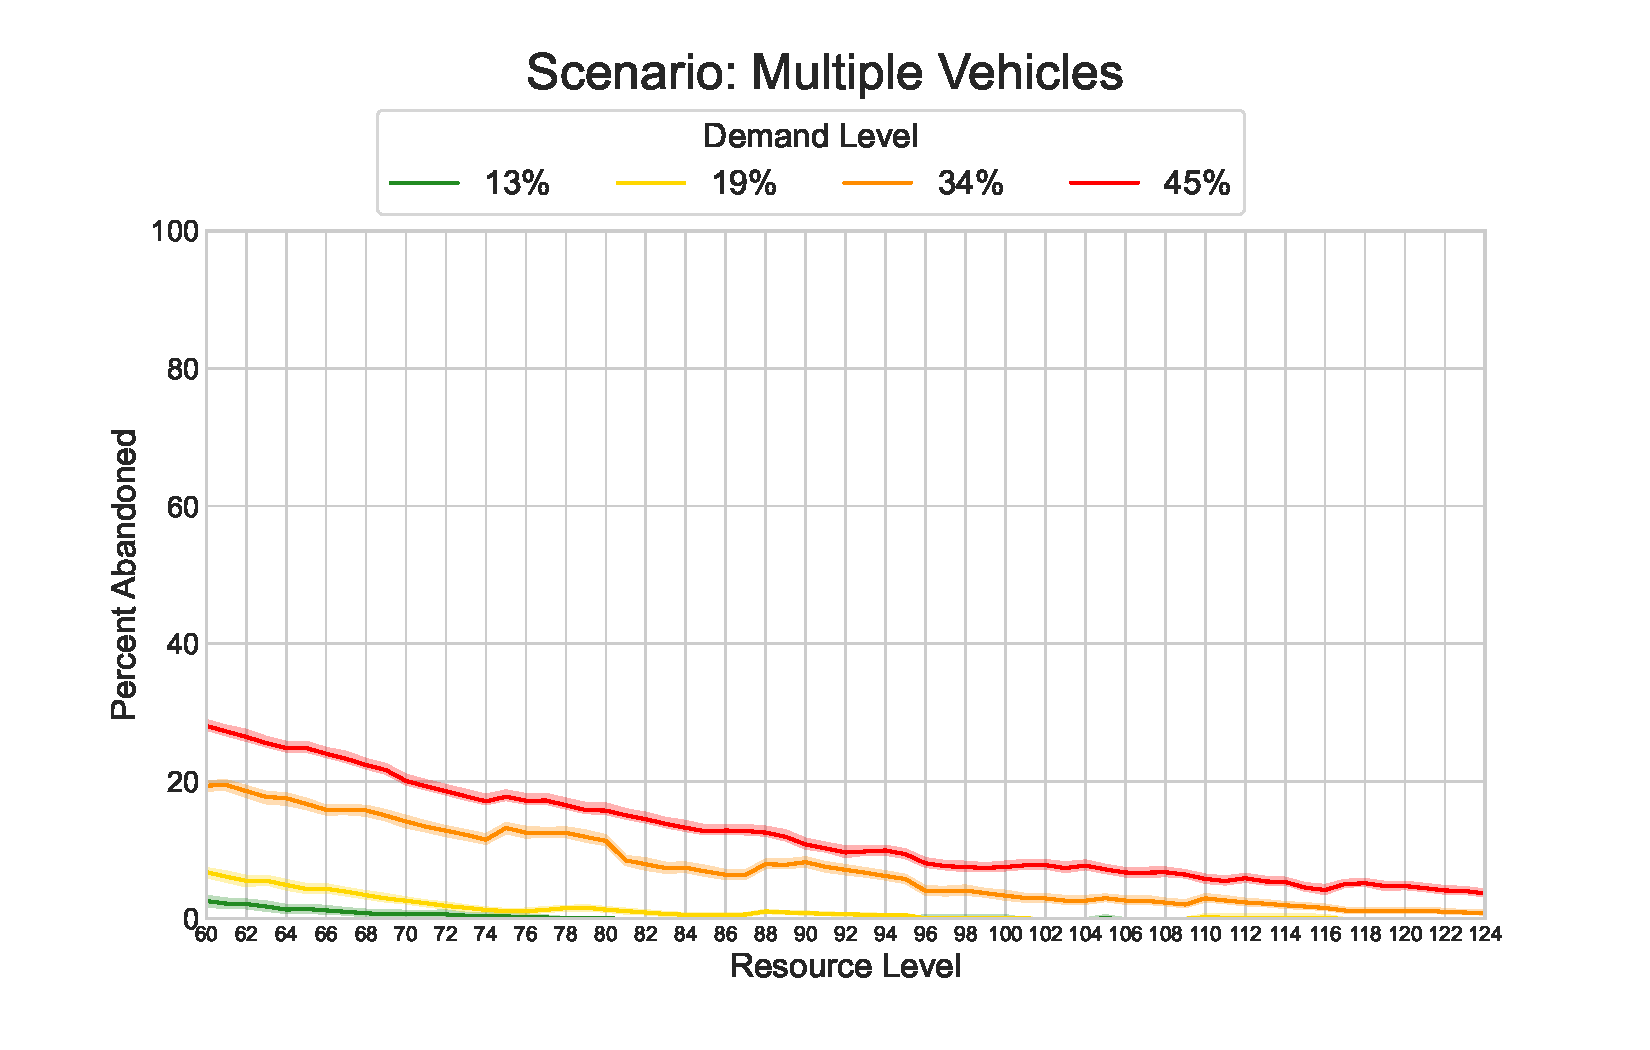
\includegraphics[width=\textwidth]{img/results/multiple_PercentAbandoned}
\caption{Multiple vehicle type scenario.}
\label{fig:results_abandoned_multiple}
\end{subfigure} 
\end{center}
\caption{Percent of abandoned calls results.}
\end{figure}

\begin{figure}
\begin{center}
\begin{subfigure}{0.48\textwidth}
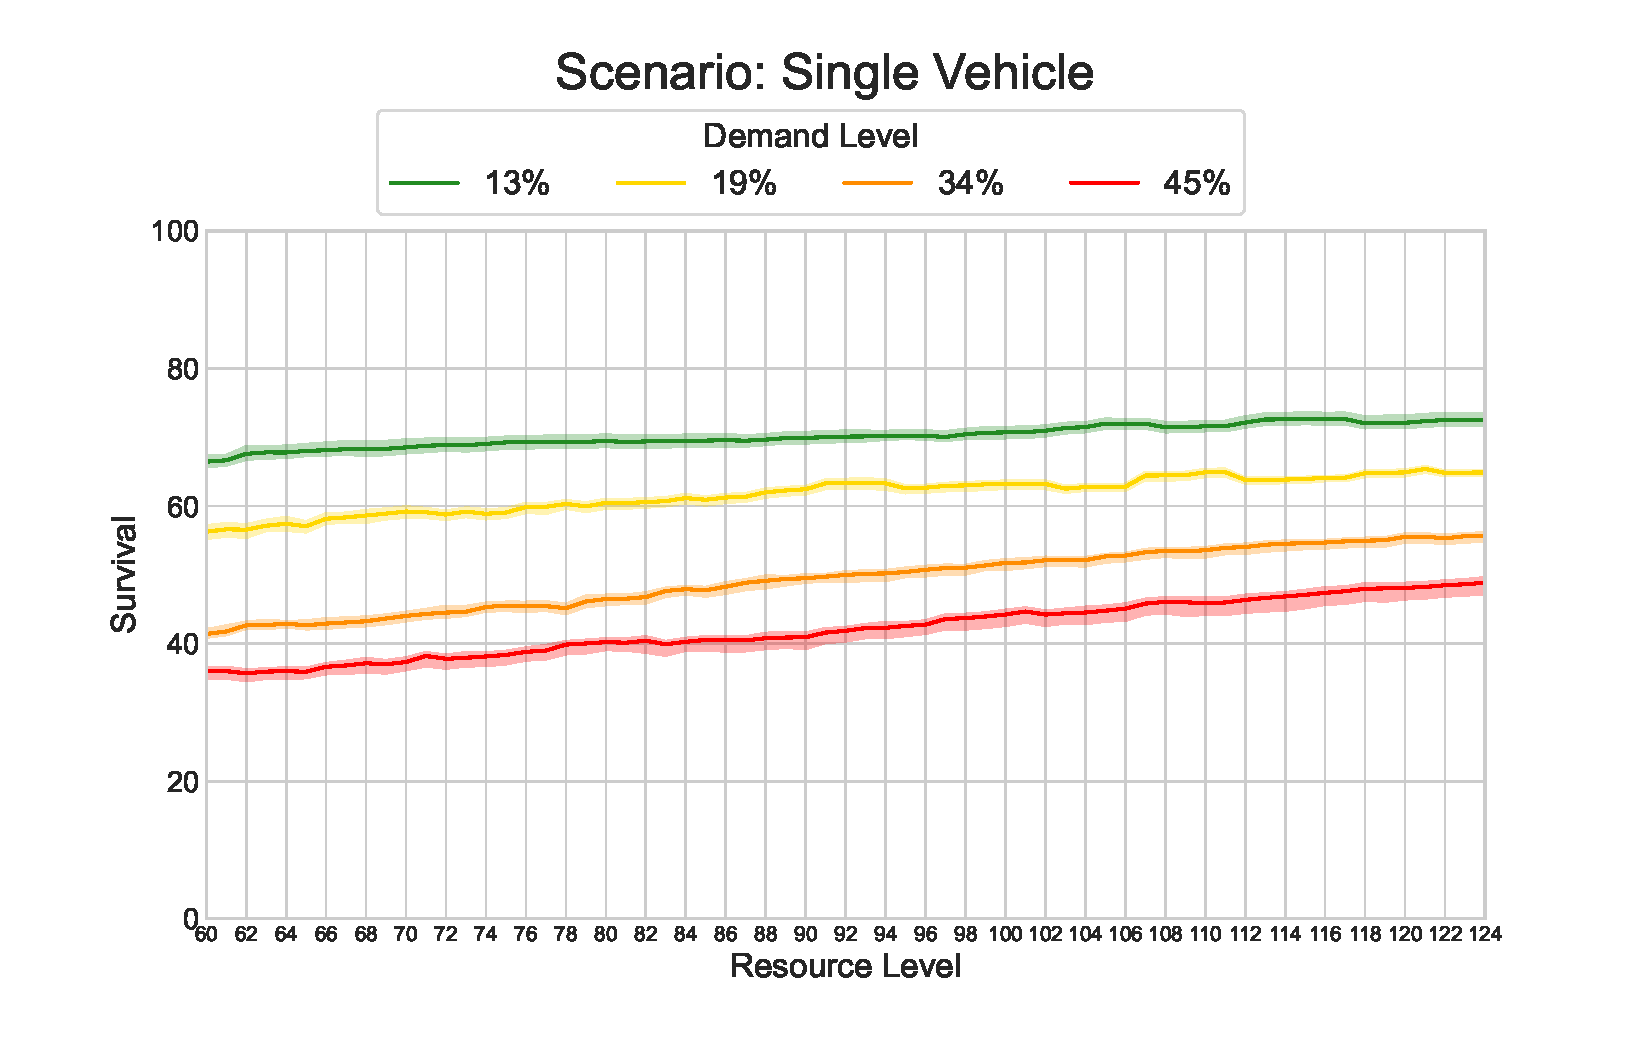
\includegraphics[width=\textwidth]{img/results/single_OverallSurvival}
\caption{Single vehicle type scenario.}
\label{fig:results_survival_single}
\end{subfigure}
\begin{subfigure}{0.48\textwidth}
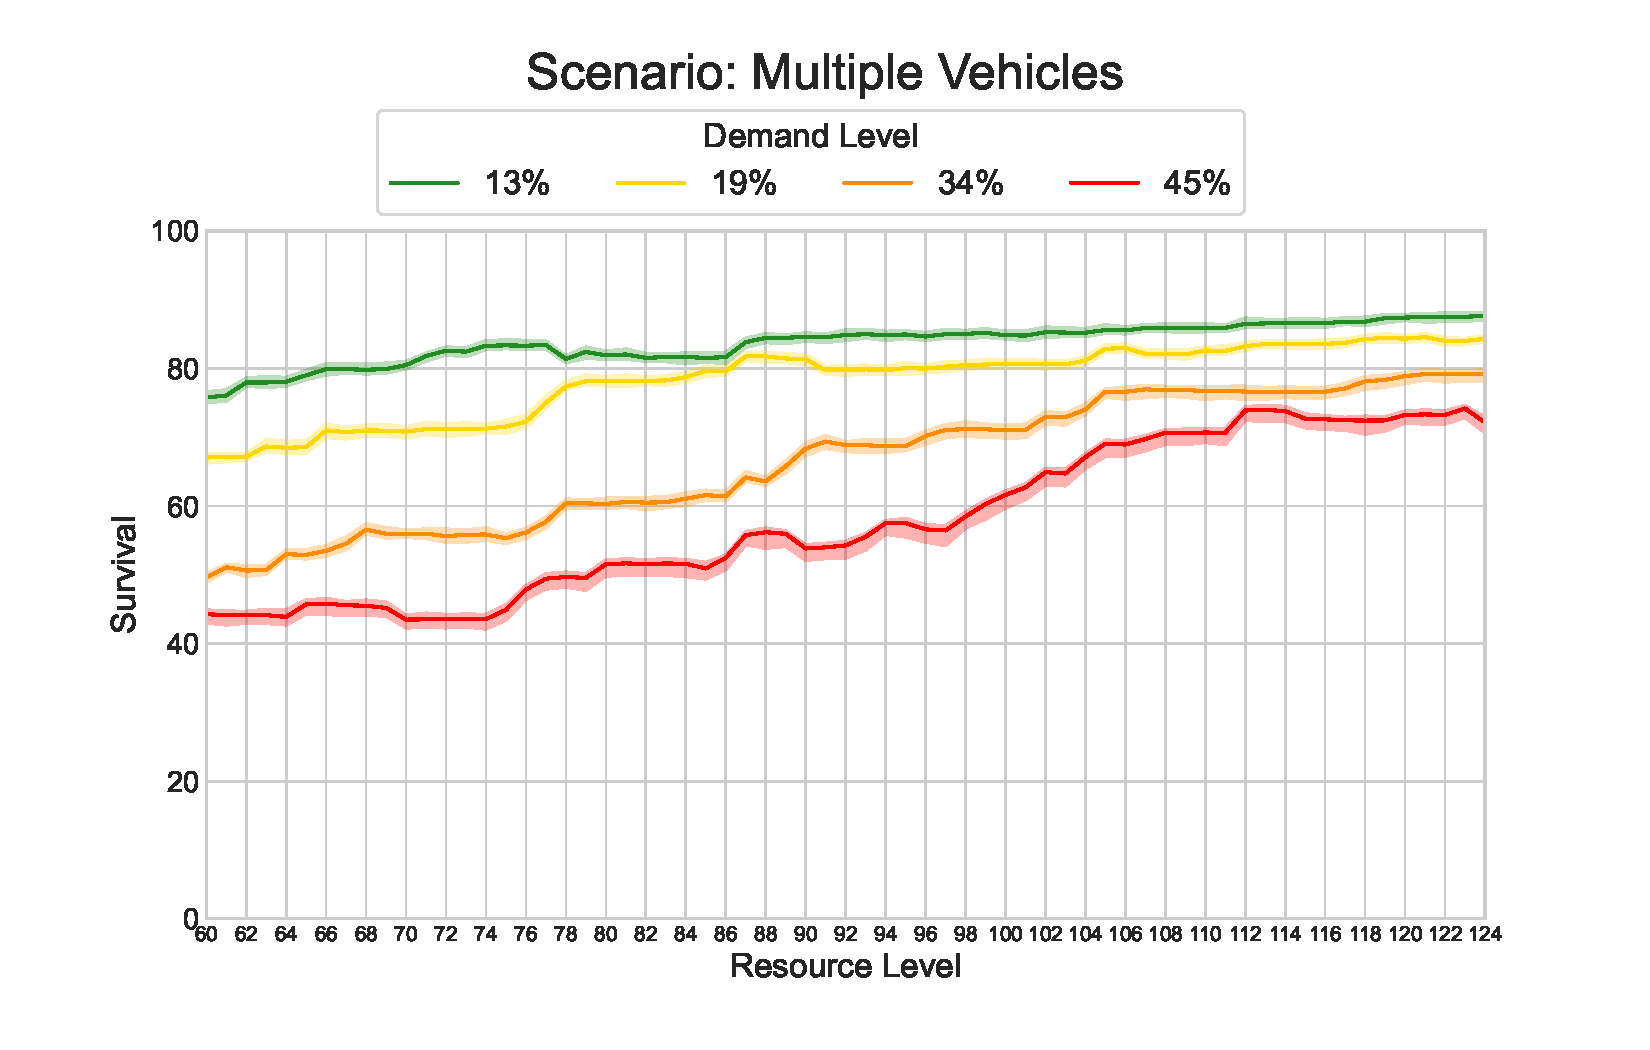
\includegraphics[width=\textwidth]{img/results/multiple_OverallSurvival}
\caption{Multiple vehicle type scenario.}
\label{fig:results_survival_multiple}
\end{subfigure}
\end{center}
\caption{Overall survival results.}
\label{fig:results_overall_survival}
\end{figure}

It is particularly interesting to compare the scenario in which single vehicle
types (only emergency ambulances) were allocated against the scenario where
multiple vehicle types (both emergency ambulances and rapid response vehicles)
were allocated. For equivalent resource levels, introducing secondary vehicles
increases ambulance utilisation, and so decreases availability, resulting in
an increase in abandoned calls. However, introducing secondary vehicles also
results in a large decrease in the mean response times, and so a large
increase in the percentage of patients seen within target.

It is also noticeable that the increases or decreases in the simulation
derived KPIs are not necessarily monotonic with increases in resource level.
This is due to the derived allocations being based on the MESLMHPHF score
only, which is a measure of survival, while the simulation derived KPIs are
indirect measures of performance. This may indicate that these indirect
measures of performance, such as mean response times or percentage within
target, are not good indicators of survival.

Crucially, the plots show that the allocations produced by the optimisation
algorithm perform better than the current allocation for the same demand and
resource levels. The current levels include 81 EAs and 13 RRVs, so a resource
level of 85.33, with multiple vehicles. Comparing the derived allocations for
this level in
Figures~\ref{fig:results_ambulance_utilisation}-\ref{fig:results_overall_survival}
to the results given in Table~\ref{tbl:current_grid_results}, the derived
allocations give lower ambulance and RRV utilisations, lower mean response
times, and a higher percentage of patients seen within target.

As experiments were run across all demand scenarios, we can see how much more
resources would be required, if optimally located, to achieve a similar level
of service as is currently offered, when demand increases.
Table~\ref{tbl:equivalent} shows, for each demand scenario, the minimum
resource level and vehicle type breakdown required to meet the current level
in each of the following KPIs: mean response time, overall survival, and
percentage of calls abandoned. For example, in order to maintain the current
75.48\% overall survival, under the demand\_19 scenario the city would require
63 EAs and 45 RRVs.
It is noticeable that fewer resources are required to maintain the current
mean response time than to maintain the current overall survival.

\begin{table}
\begin{center}
\resizebox{\textwidth}{!}{%
\begin{tabular}{cccc}
\toprule
Demand Scenario & Mean Response Time & Overall Survival & Percent Abandoned \\
\midrule
\textbf{demand\_13} & 60, (50, 30) & 60, (50, 30) & 80, (66, 42) \\
\textbf{demand\_19} & 70, (60, 30) & 78, (63, 45) & 101, (79, 66) \\
\textbf{demand\_34} & 88, (75, 39) & 106, (83, 69) & $>$ 124 \\
\textbf{demand\_45} & 99, (85, 42) & $>$ 124 & $>$ 124 \\
\midrule
Current Level & 16.8 minutes & 75.48\% & 0.0339\% \\
\bottomrule
\end{tabular}%
}
\caption{Resources required to maintain current KPI levels when optimising
         locations under the four demand scenarios.}
\label{tbl:equivalent}
\end{center}
\end{table}



\section{Discussion \& Conclusions}\label{sec:discussion}
This paper has described the development of EMS demand and capacity models and
their application to the city of Jakarta, Indonesia. To our knowledge, this is
the first such study of analysing emergency ambulance services in Jakarta, and
the work has directly assisted and guided providers and the government to make
investment decisions for a coordinated and free to use EMS.

Firstly, we have considered patient survival and outcomes within a developed
MESLMHPHF model. By considering geospatial travel times and accounting for the
varying needs of different patient types though categorising patients by
speciality and through using different survival function profiles, an expected
overall survival was given. This could be used within a optimisation
processes, in this case by using a population-based neighbourhood search
evolutionary heuristic, to find vehicle fleet allocations that maximise
expected survival. This expected survival function extends previous work in
\cite{Knight2012918} to include more than one vehicle type.
A particular novelty here was numerically solving utilisation relationships,
Equations~\ref{eqn:utilisations_primary} and~\ref{eqn:utilisations_secondary},
to calculate the expected survival.

Secondly, a discrete event simulation model has been used to evaluate existing
and potential heterogeneous vehicle ambulance feet allocations in terms of key
performance measures, such as response times, survival, and vehicle
utilisation rates. This takes into consideration geospatial demand and travel,
and temporal variation in demand and traffic levels. A novel feature of our
approach is that the model comprises of sequential simulations, feeding data
directly from one into the other in order to simulate primary and secondary
vehicles separately while maintaining synchronicity, with the overall aim of
reducing the complexity of the simulation logic.

Both models investigate ambulance service activity in the case of
heterogeneous patients and heterogeneous fleets. Heterogeneous patient groups
consider those with distinct demand profiles, priorities, and survival
functions. Heterogeneous fleets concern different types of vehicles, in our
case emergency ambulances (EAs) which respond to every patient, and Rapid
Response Vehicles (RRVs) which can be utilised to reach patients faster,
despite being unable to transport patients themselves.

Using a combination of models has permitted an approach that can capture
performance measures or take into account factors that each model in isolation
can not. For example, the maximum expected survival model is a lot more
appropriate for use within an optimisation process as the runtimes are a far
more reasonable than the simulation. On the other hand, the simulation allows
for greater complexity such as temporal demand, and is able to capture a
greater range of KPIs.

A key feature of both models, and their novelty, is the consideration of
heterogeneous fleets. In a highly populated area such as Jakarta (around
16,000 population per km$^2$), the inclusion of RRVs such as paramedics on
motorbikes is very important, given RRVs can access areas that cannot easily
or quickly be accessed by ambulances. Results from both the optimisation and
simulation research showed that the RRVs can help increase the overall
survival and reduce the response times, especially crucial when responding to
life threatening events such as cardiac arrests \cite{holmen2020shortening}. 

The results of our research also suggest that allocation strategies may not be
intuitive to ambulance service managers, further emphasising the value of a
modelling approach. For example, senior managers suggested the use of a grid
allocation to maximise geographic coverage, with ambulances equally spread
across the city. This was shown to be sub-optimal because neighbourhoods have
different population densities and characteristics. For example, the number of
daily commuters in Jakarta is considerably high during day time due to work
and education \cite{BPS_Jakarta_migrasi}. Municipalities where trading,
educational institutions, and offices are concentrated may become more
populated during day time. The model has quantified the deterioration in
response times and patient outcomes should a fixed grid system be implemented,
leading to 119 to drop this consideration.

The ambulance posts in Jakarta depend on the service provider. Those
ambulances provided by the government are in various locations including
government buildings as well as community clinics and sub-district hospitals.
In our case, we used current ambulance posts as the locations for allocating
the resources. As demands for ambulances may change from time to time, future
work could evaluate different, and perhaps dynamic, ambulance posts that
depend on changing demand volumes in neighbourhoods by time of the day.

The data used for ambulance demand covered one year from 1 January to 31
December 2019, prior the COVID-19 pandemic. Recent studies related to
ambulance demand indicate that the  pandemic has severely impacted on the
utilisation of EMS, for examples in call volumes \cite{csan2021effects} and in
specific medical conditions such as trauma \cite{ azbel2021effects}, and
possibly still continue to affect demand. Ambulance providers, such as 118 and
119, may use our modelling tools to incorporate future demand data and
re-evaluate resource needs. To aid this, we are currently working on
interfacing the simulation and optimisation into a single easy to use decision
support tool with a dashboard (data visualiser). 

Studies have shown that the quality in pre-hospital data collection varies
considerably in Indonesia \cite{hooper2019_datacollection}. We encountered
similar challenges and have suggested to 119 and the Indonesian Government
that they should continue to strive to improve the coverage and quality of
data collection. Future work could explore in more depth unmet demand that is
not recorded in the ED or in the ambulance data.

Indonesia is a vast country with an uneven population density and varying
quality of available healthcare resources. The models have been parameterised
with data from a high population, high density urban area which is also
relatively well resourced with healthcare facilities compared to other regions
in the country. Ambulance services in rural areas of Indonesia may not have
the same quality in management and organisation compared to the capital,
Jakarta. We intend to conduct future studies to apply the developed models to
analyse ambulance demand and allocations in different areas of Indonesia,
including in rural regions.

In conclusion, the developed models have demonstrated a novel approach in
modelling ambulance allocations that incorporate multiple vehicle types and
health conditions, whilst also capturing patient survival. Our work has
already informed major decisions on the design of a free to use and
coordinated EMS system for Jakarta. Ongoing collaboration will continue to
assist ambulance providers and the Indonesian Government in providing
evidence-based decision making for the benefit of patients and the population
they serve, including the exploration of the roll-out of 119 beyond Jakarta to
other regions of Indonesia. 



% \section*{CRediT authorship contribution statement}
% From Computers and OR, select from:\\

% Conceptualisation; Funding acquisition; Investigation; Methodology; Project administration; Resources; Software; Supervision; Validation; Writing - original draft; Writing - review \& editing.\\


% {\bf Geraint Palmer:} Conceptualisation, Investigation, Methodology, Software, Writing – original draft\\
% {\bf Sarie Brice:} Conceptualisation, Investigation, Methodology, Writing – original draft\\
% {\bf Daniel Gartner:} Conceptualisation, Funding acquisition, Methodology, review \& editing.\\
% {\bf Paul Harper:} Conceptualisation, Investigation, Methodology, Funding acquisition, Resources, Project administration, Writing – review \& editing.\\
% {\bf Vince Knight:} Conceptualisation, Funding acquisition, Investigation, Methodology, Software, review \& editing.\\
% {\bf Leanne Smith:} Methodology.\\
% {\bf Mark Tuson:} Conceptualisation, Investigation, Methodology, Software, Writing – original draft\\



\section*{Acknowledgements}
The study was funded by EPSRC with grant no: EP/T003197/1. We would like to
express our sincere gratitude to Indonesian emergency ambulance providers
including 118 and 119 for their support, insights and provision of data. In
particular we wish to thank Professor Aryono Djuned Pusponegoro and Ms Asti
Puspita Rini, Founder and Director of 118 Ambulance Service Foundation and Dr
Winarto, Head of the 119 Ambulance Service in Jakarta.


\appendix

\section{Annotated Objective Function}\label{apx:annotated}
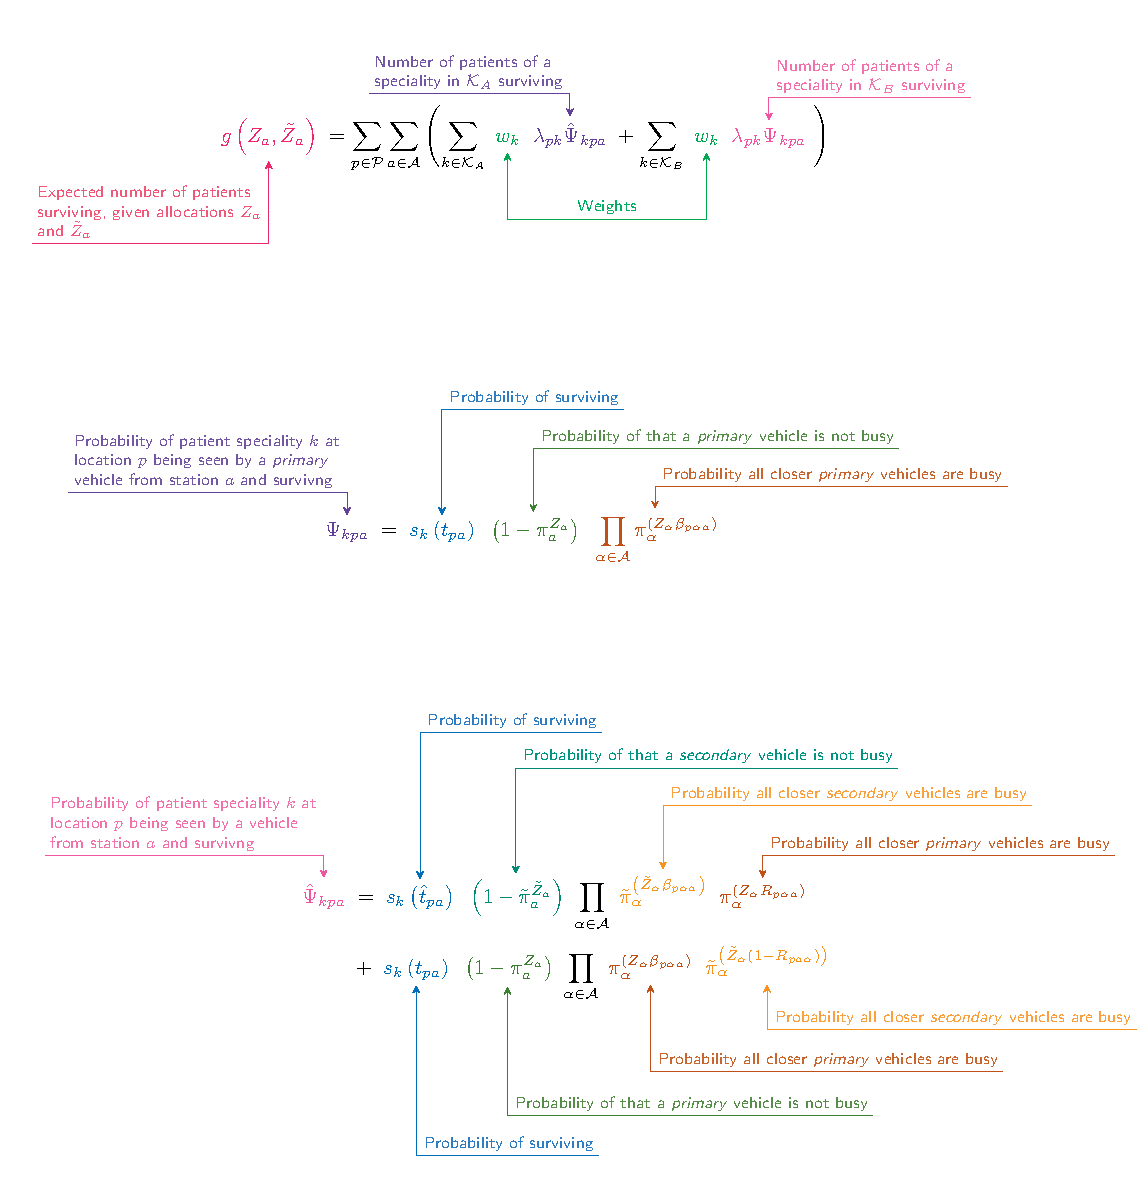
\includegraphics[width=\textwidth]{img/annotate}


\section{Model Parameters}\label{apx:parameters}
Call arrival rates $\lambda_{pk}$ are derived from 2019 demand data slit by
municipality and speciality, and time of day. Probabilities $q_{pky}$ are
similarly derived from the 2019 data of transit journeys. All traffic-free
travel times are found using Google Maps API, while time-dependent traffic
delays are found from the TomTom website and given in
Table~\ref{tbl:delay_factors}.

\begin{table}
\begin{center}
\begin{tabular}{ccccc}
\toprule
$h$ & 0000-0500 & 0500-1500 & 1500-1800 & 1800-0000 \\
\midrule
$d_h$ & 0.98 & 0.66 & 0.59 & 0.77 \\
$\tilde{d}_h$ & 1.96 & 0.91 & 0.83 & 1.16 \\
\bottomrule
\end{tabular}
\end{center}
\caption{Primary and secondary delay factors.}
\label{tbl:delay_factors}
\end{table}

The other models are parameterised in the following way:
\begin{itemize}
  \item From a sample of calls the time at site $G_k$ was found to follow a
        lognormal distribution with parameters $\mu=-0.6219$ and $\sigma=0.8048$.
        For the case of Jakarta this was modelled identically for all
        specialities $k$. Comparison between the lognormal fit and the sampled
        times are given in Figure~\ref{fig:lognorm_fit}.
  \item From discussions with staff at the ambulance service in Jakarta, the
        time at hospital $J_k$ was modelled as a Uniform distribution between
        40 and 60 minutes for the emergency specialities A1 and A2, and
        between 20 and 30 minutes for non-emergency speciality B.
  \item From discussions with staff at the ambulance service in Jakarta, the
        refill time $\Theta$ is taken to be 60 minutes for an emergency
        ambulance, and 15 minutes for an RRV.
\end{itemize}

\begin{figure}[ht]
\centering
  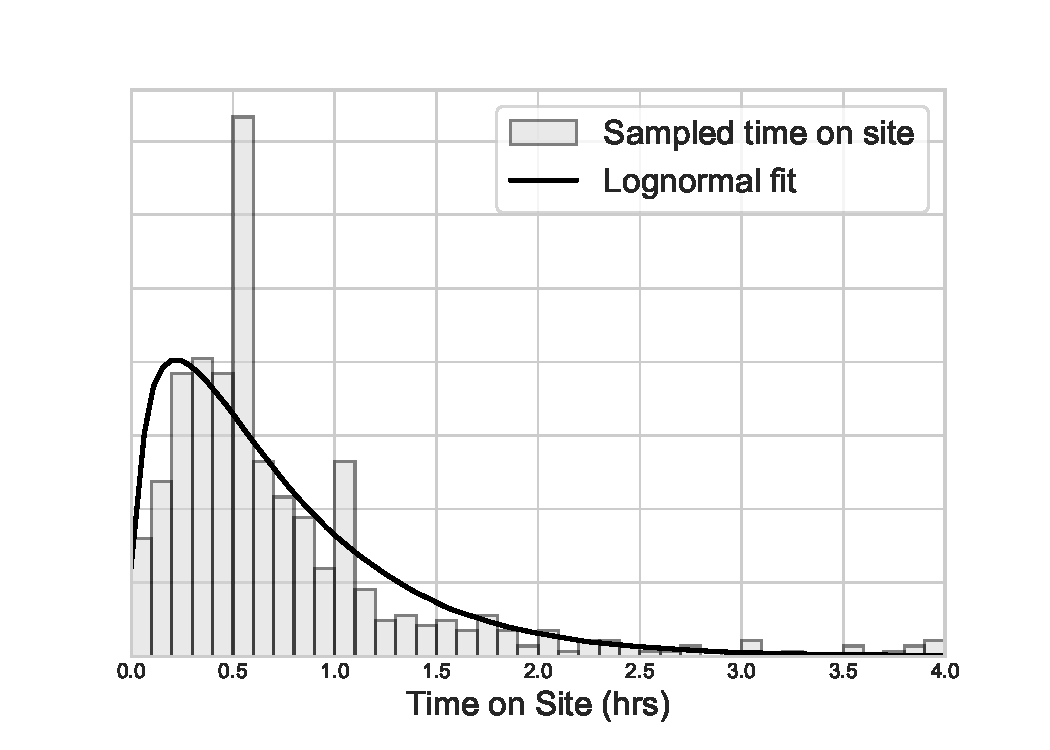
\includegraphics[width=0.6\textwidth]{img/time_on_site_fit.pdf}
    \caption{Comparison between the sampled time on site and the lognormal
             fit.}
  \label{fig:lognorm_fit}
\end{figure}


\section{Exploration of Optimisation Hyperparameters}\label{apx:hyperparameters}
Figure~\ref{fig:hyperparameters_exploration} shows the performance of the
population-based neighbourhood search evolutionary heuristic algorithm under
different values of the hyperparameters $N$, $\kappa$, $m_0$, and $c$.

\begin{figure}[ht]
\centering
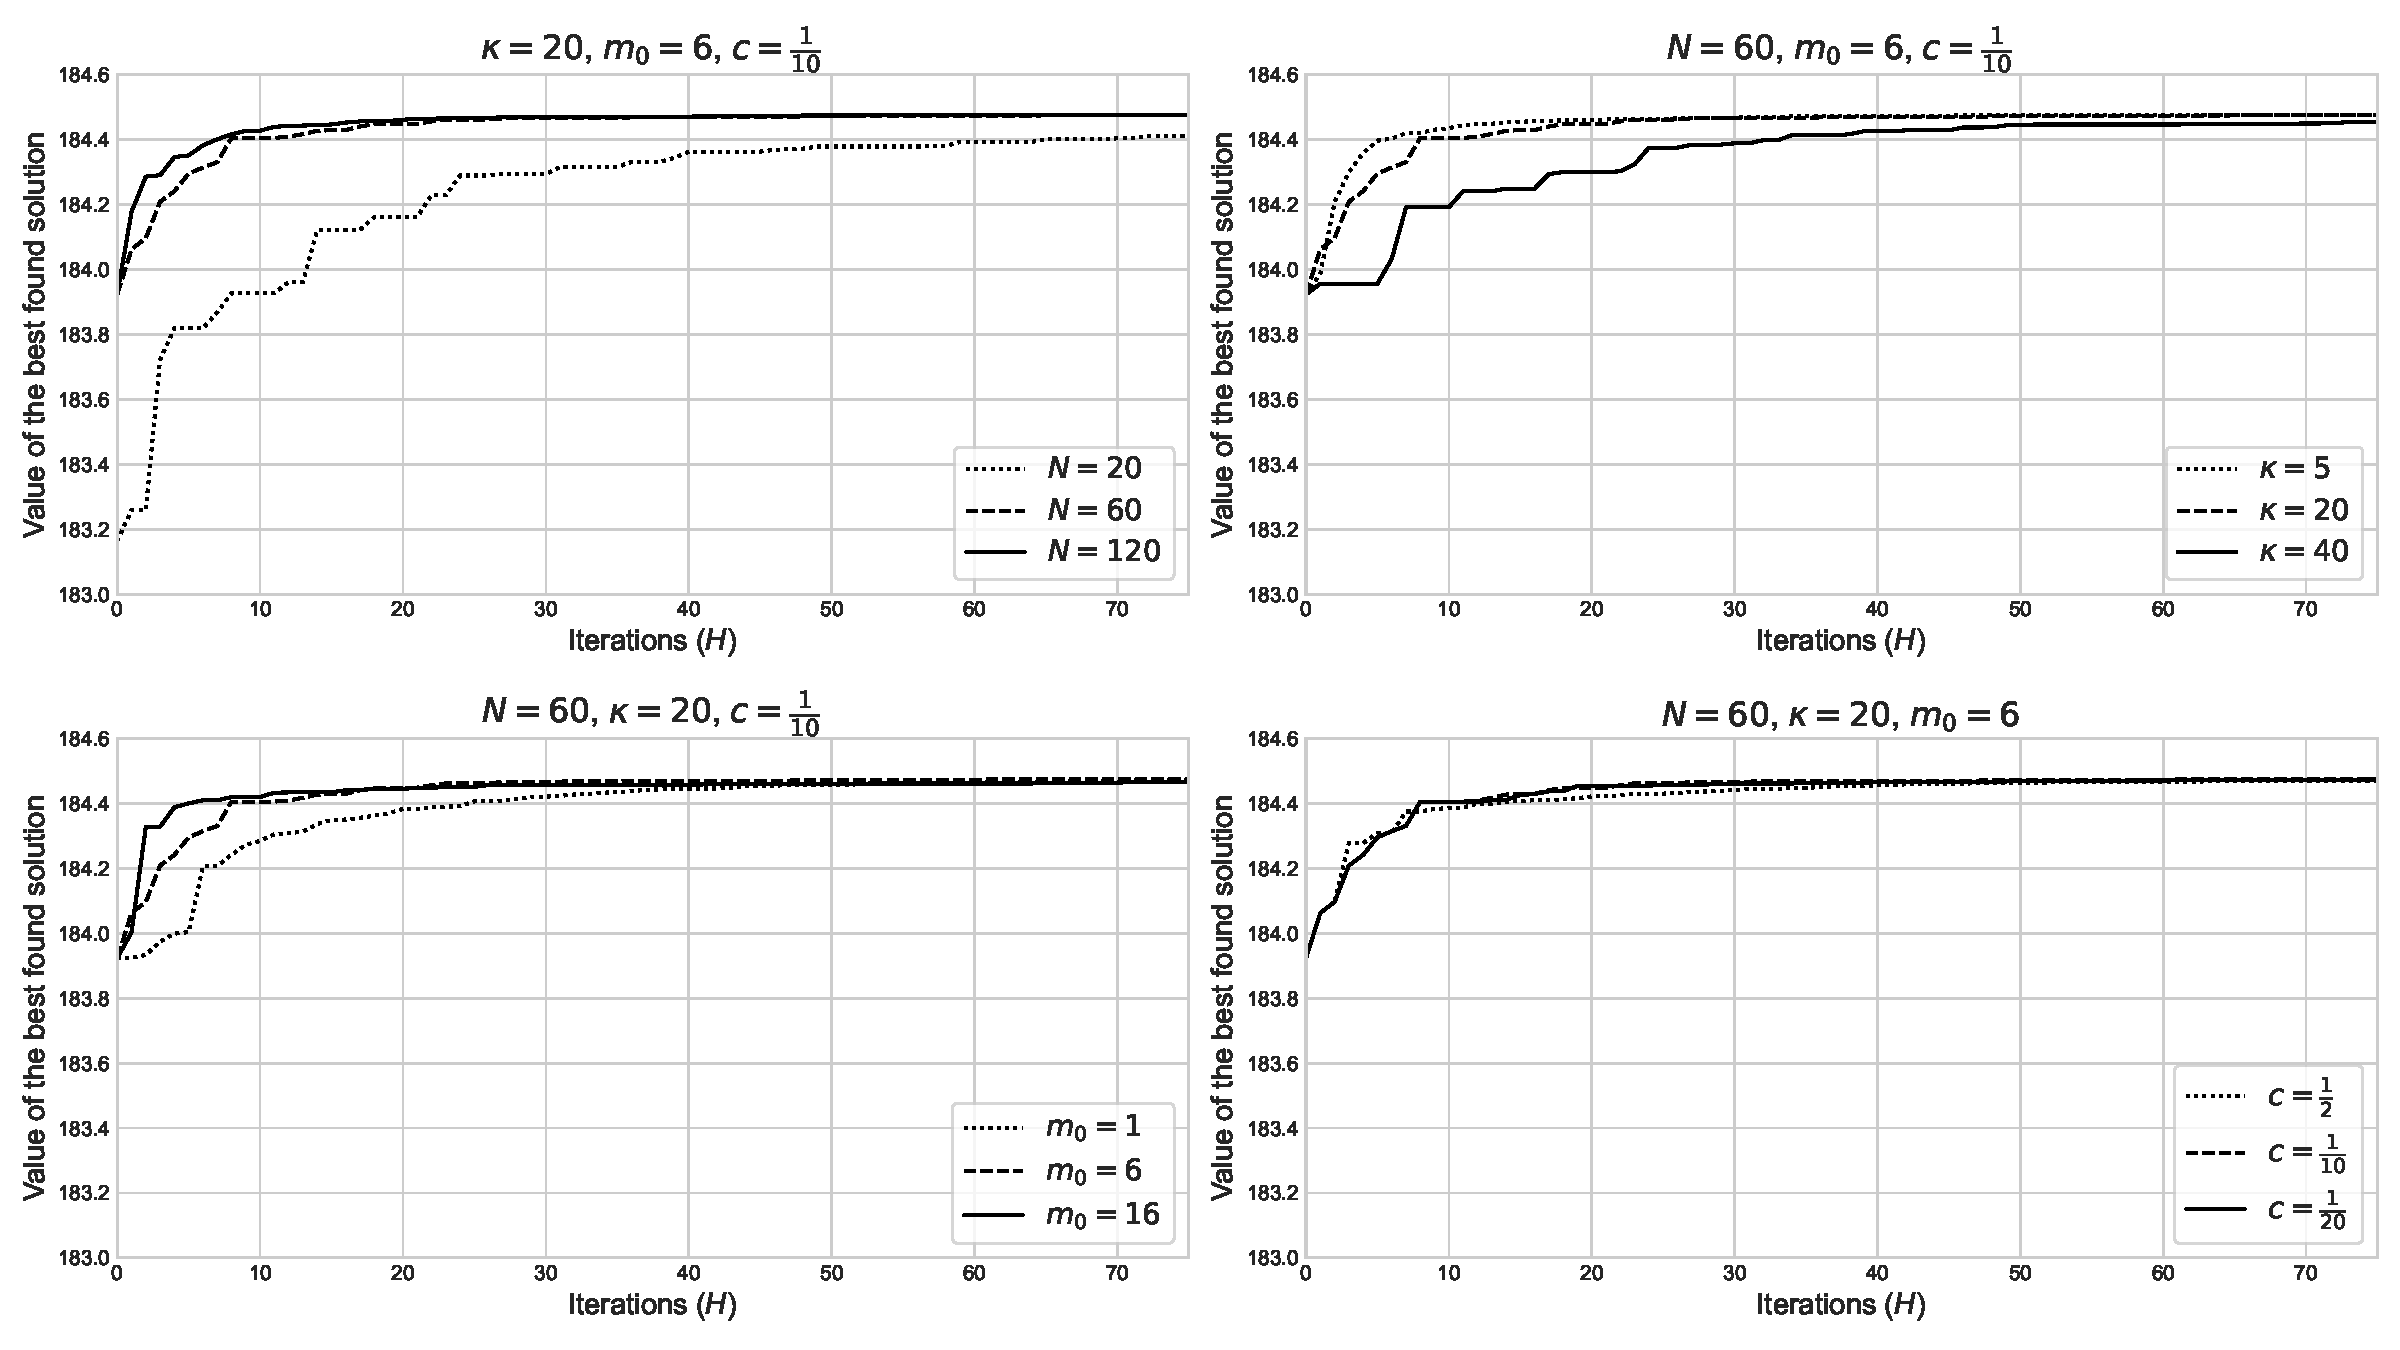
\includegraphics[width=\textwidth]{img/hyperparameter_exploration}
\caption{Comparison between optimisation performance for low, medium, and high
values of $N$, $\kappa$, $m_0$, and $c$. Optimisation is run on demand
scenario 19, for 70 primary and 30 secondary vehicles.}
\label{fig:hyperparameters_exploration}
\end{figure}


\section{Optimised Allocations for Current Vehicle Numbers}
Figures~\ref{fig:optimal_current_allocation_13},
\ref{fig:optimal_current_allocation_19}, \ref{fig:optimal_current_allocation_34}
and~\ref{fig:optimal_current_allocation_45} show the optimised allocations for
81 primary and 13 secondary vehicles under demand scenarios \textbf{D13},
\textbf{D19}, \textbf{D34}, and \textbf{D45} respectively.

\begin{figure}
\begin{center}
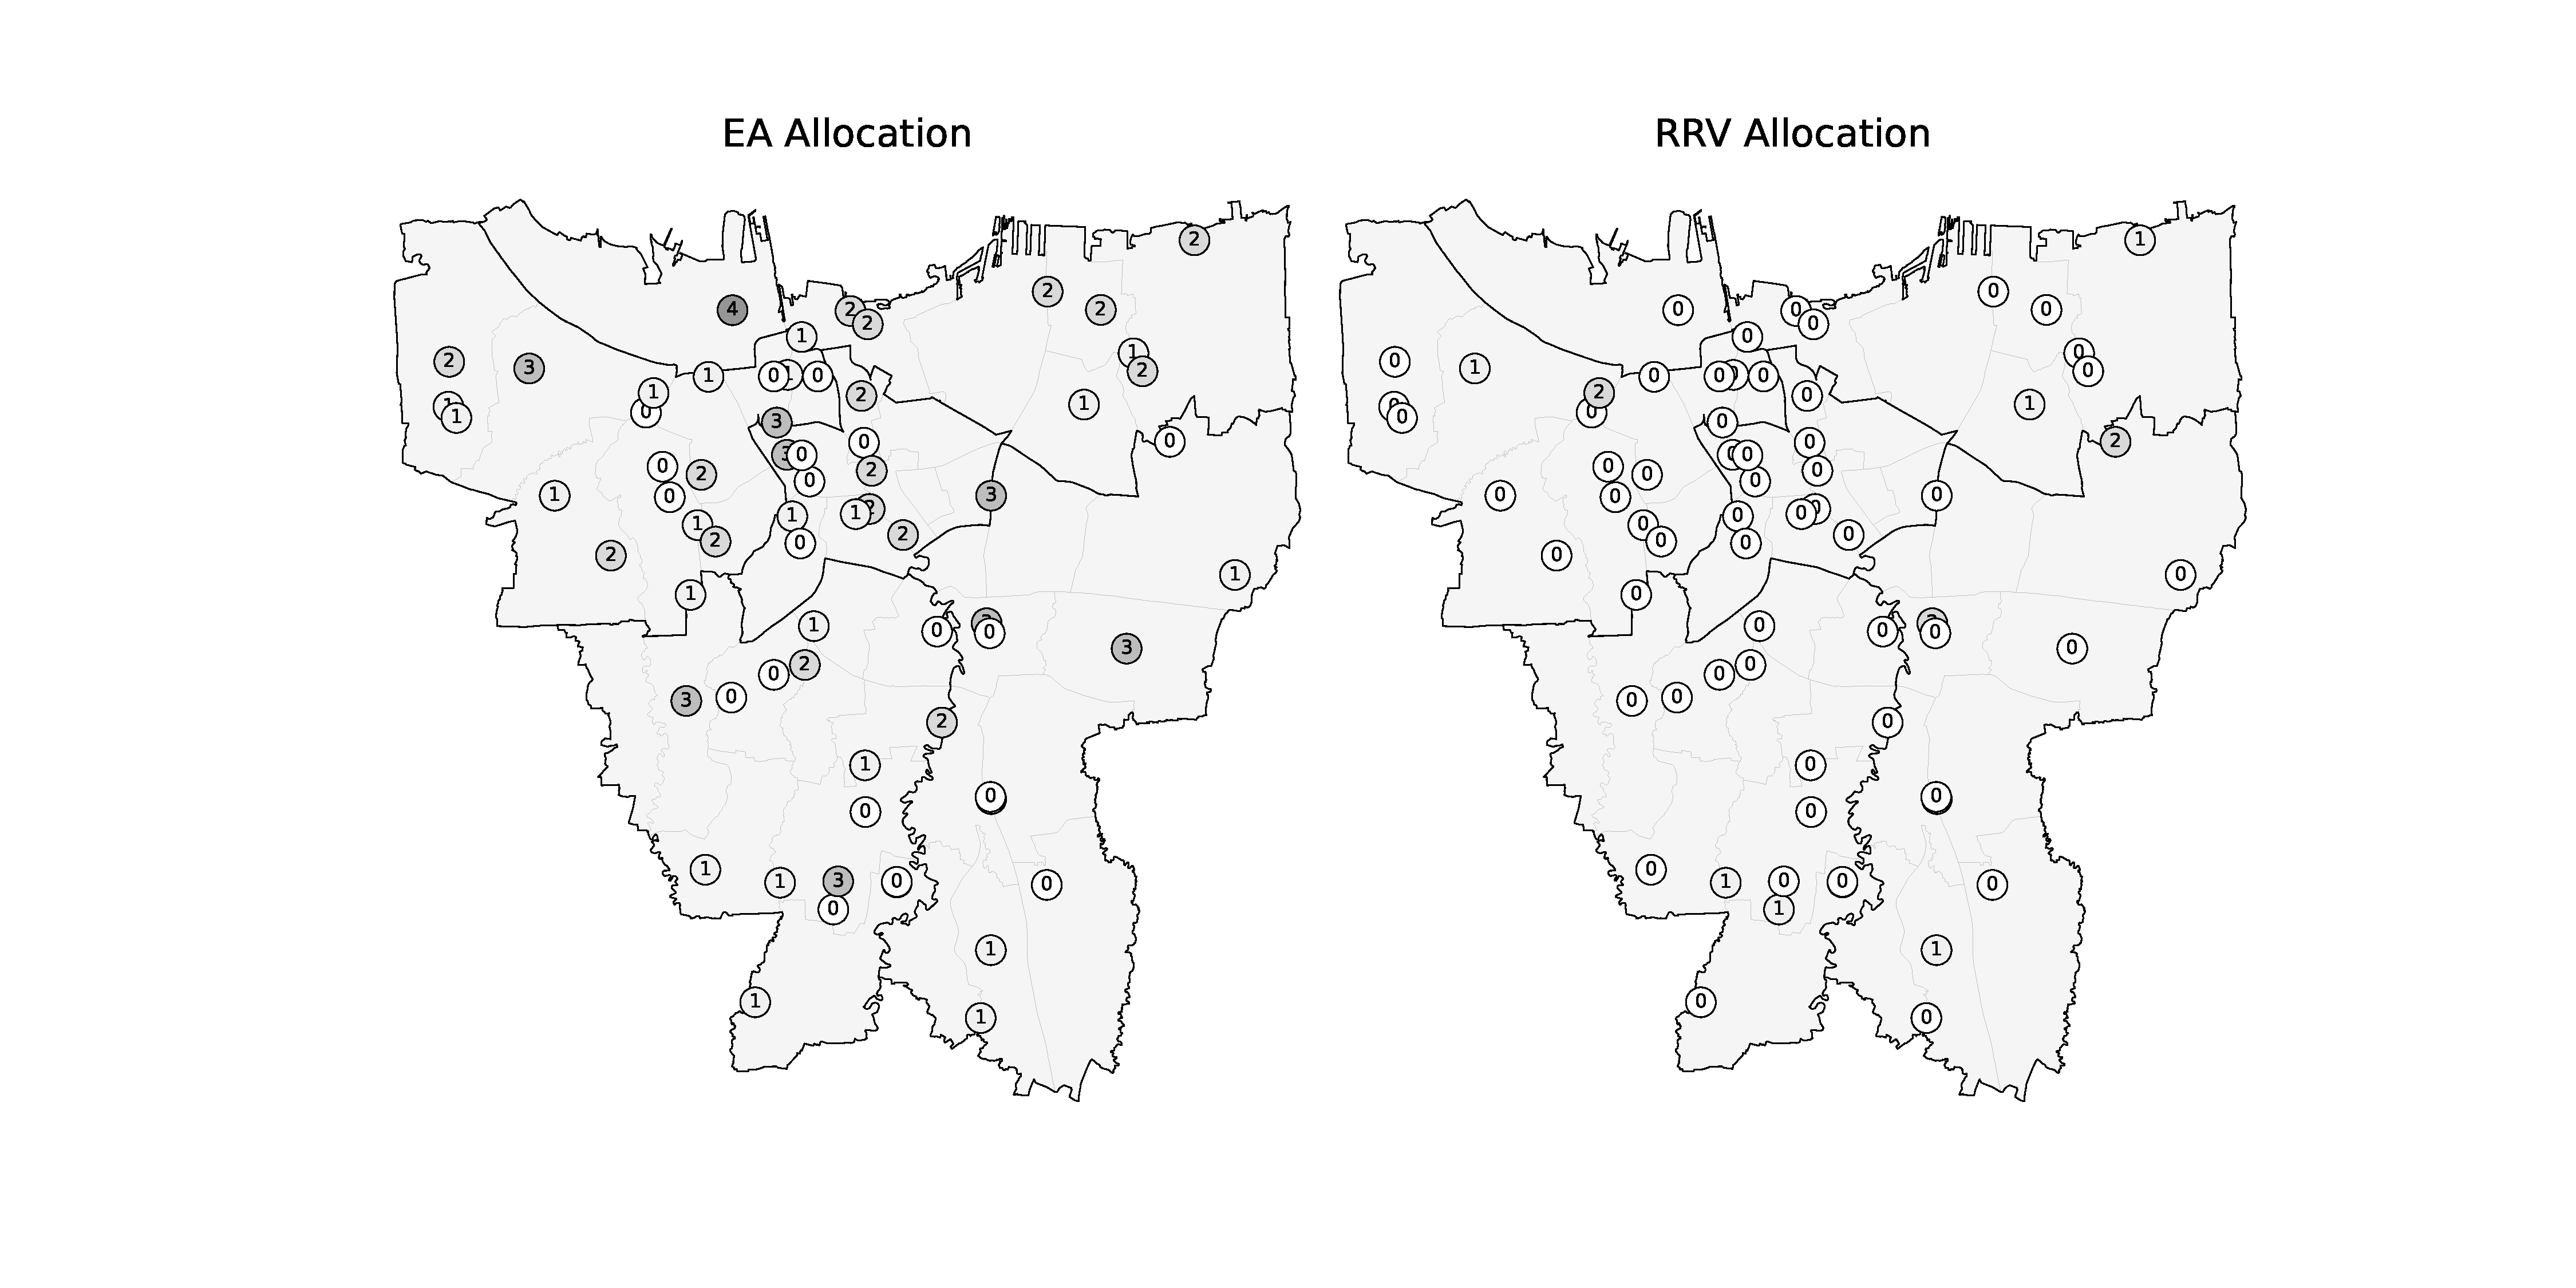
\includegraphics[width=\textwidth]{img/map_optimised_13}
\caption{Optimised allocation of 81 EAs and 13 RRVs, under scenario \textbf{D13}.}
\label{fig:optimal_current_allocation_13}
\end{center}
\end{figure}

\begin{figure}
\begin{center}
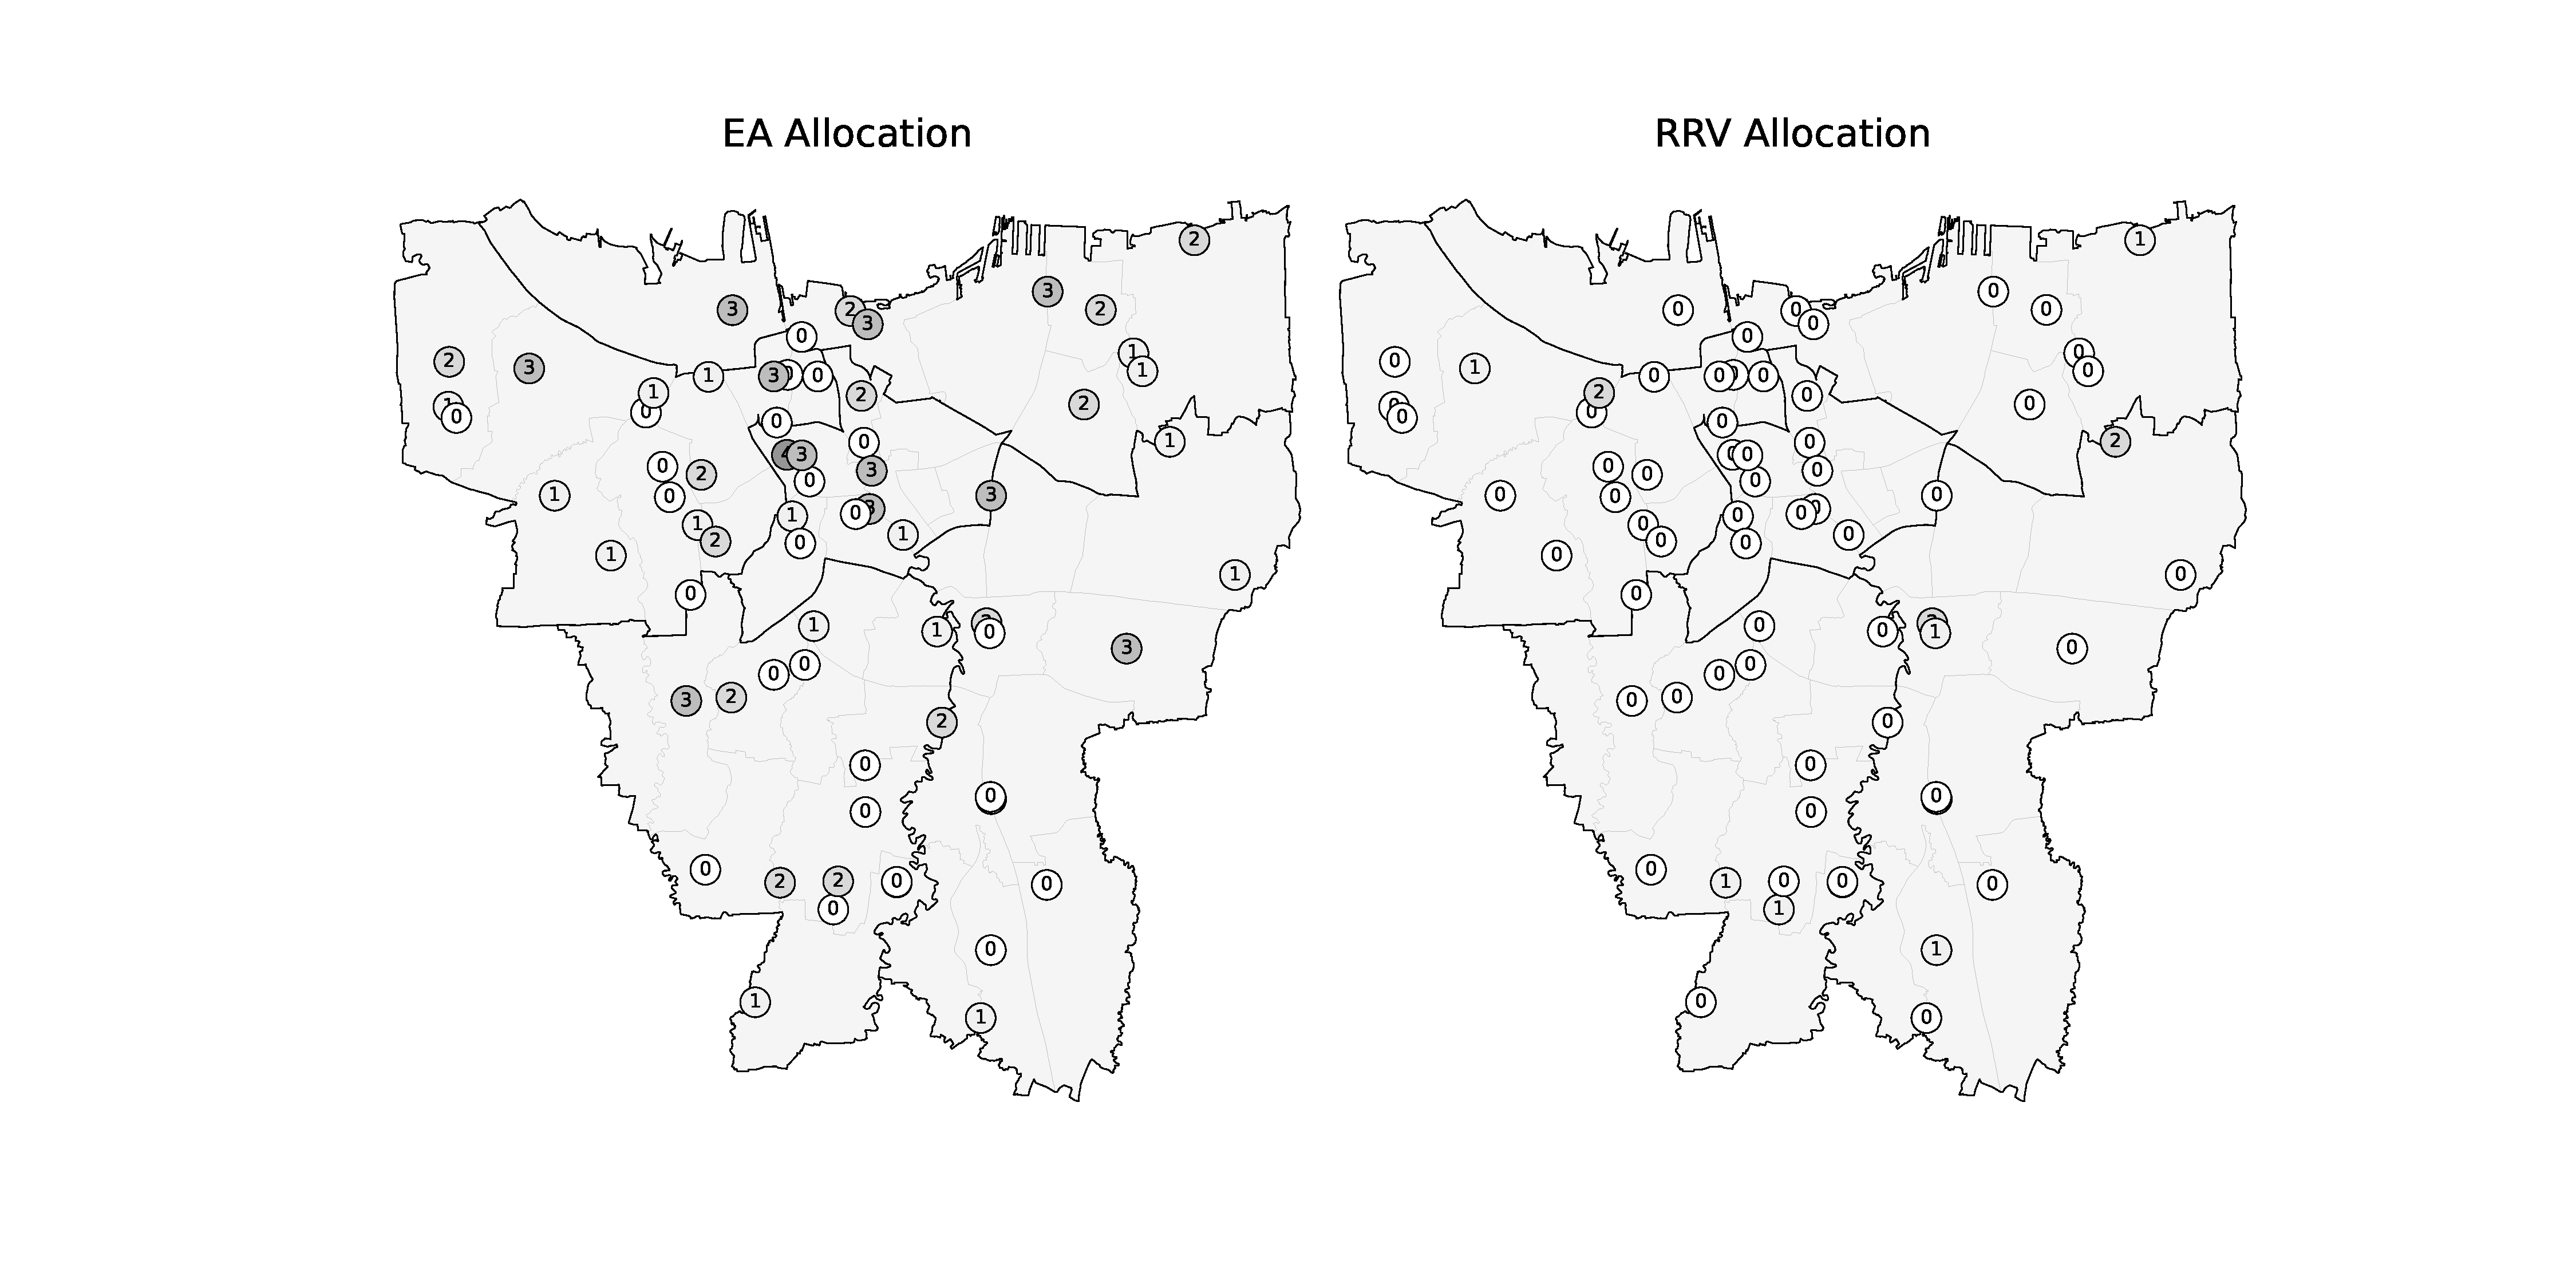
\includegraphics[width=\textwidth]{img/map_optimised_19}
\caption{Optimised allocation of 81 EAs and 13 RRVs, under scenario \textbf{D19}.}
\label{fig:optimal_current_allocation_19}
\end{center}
\end{figure}

\begin{figure}
\begin{center}
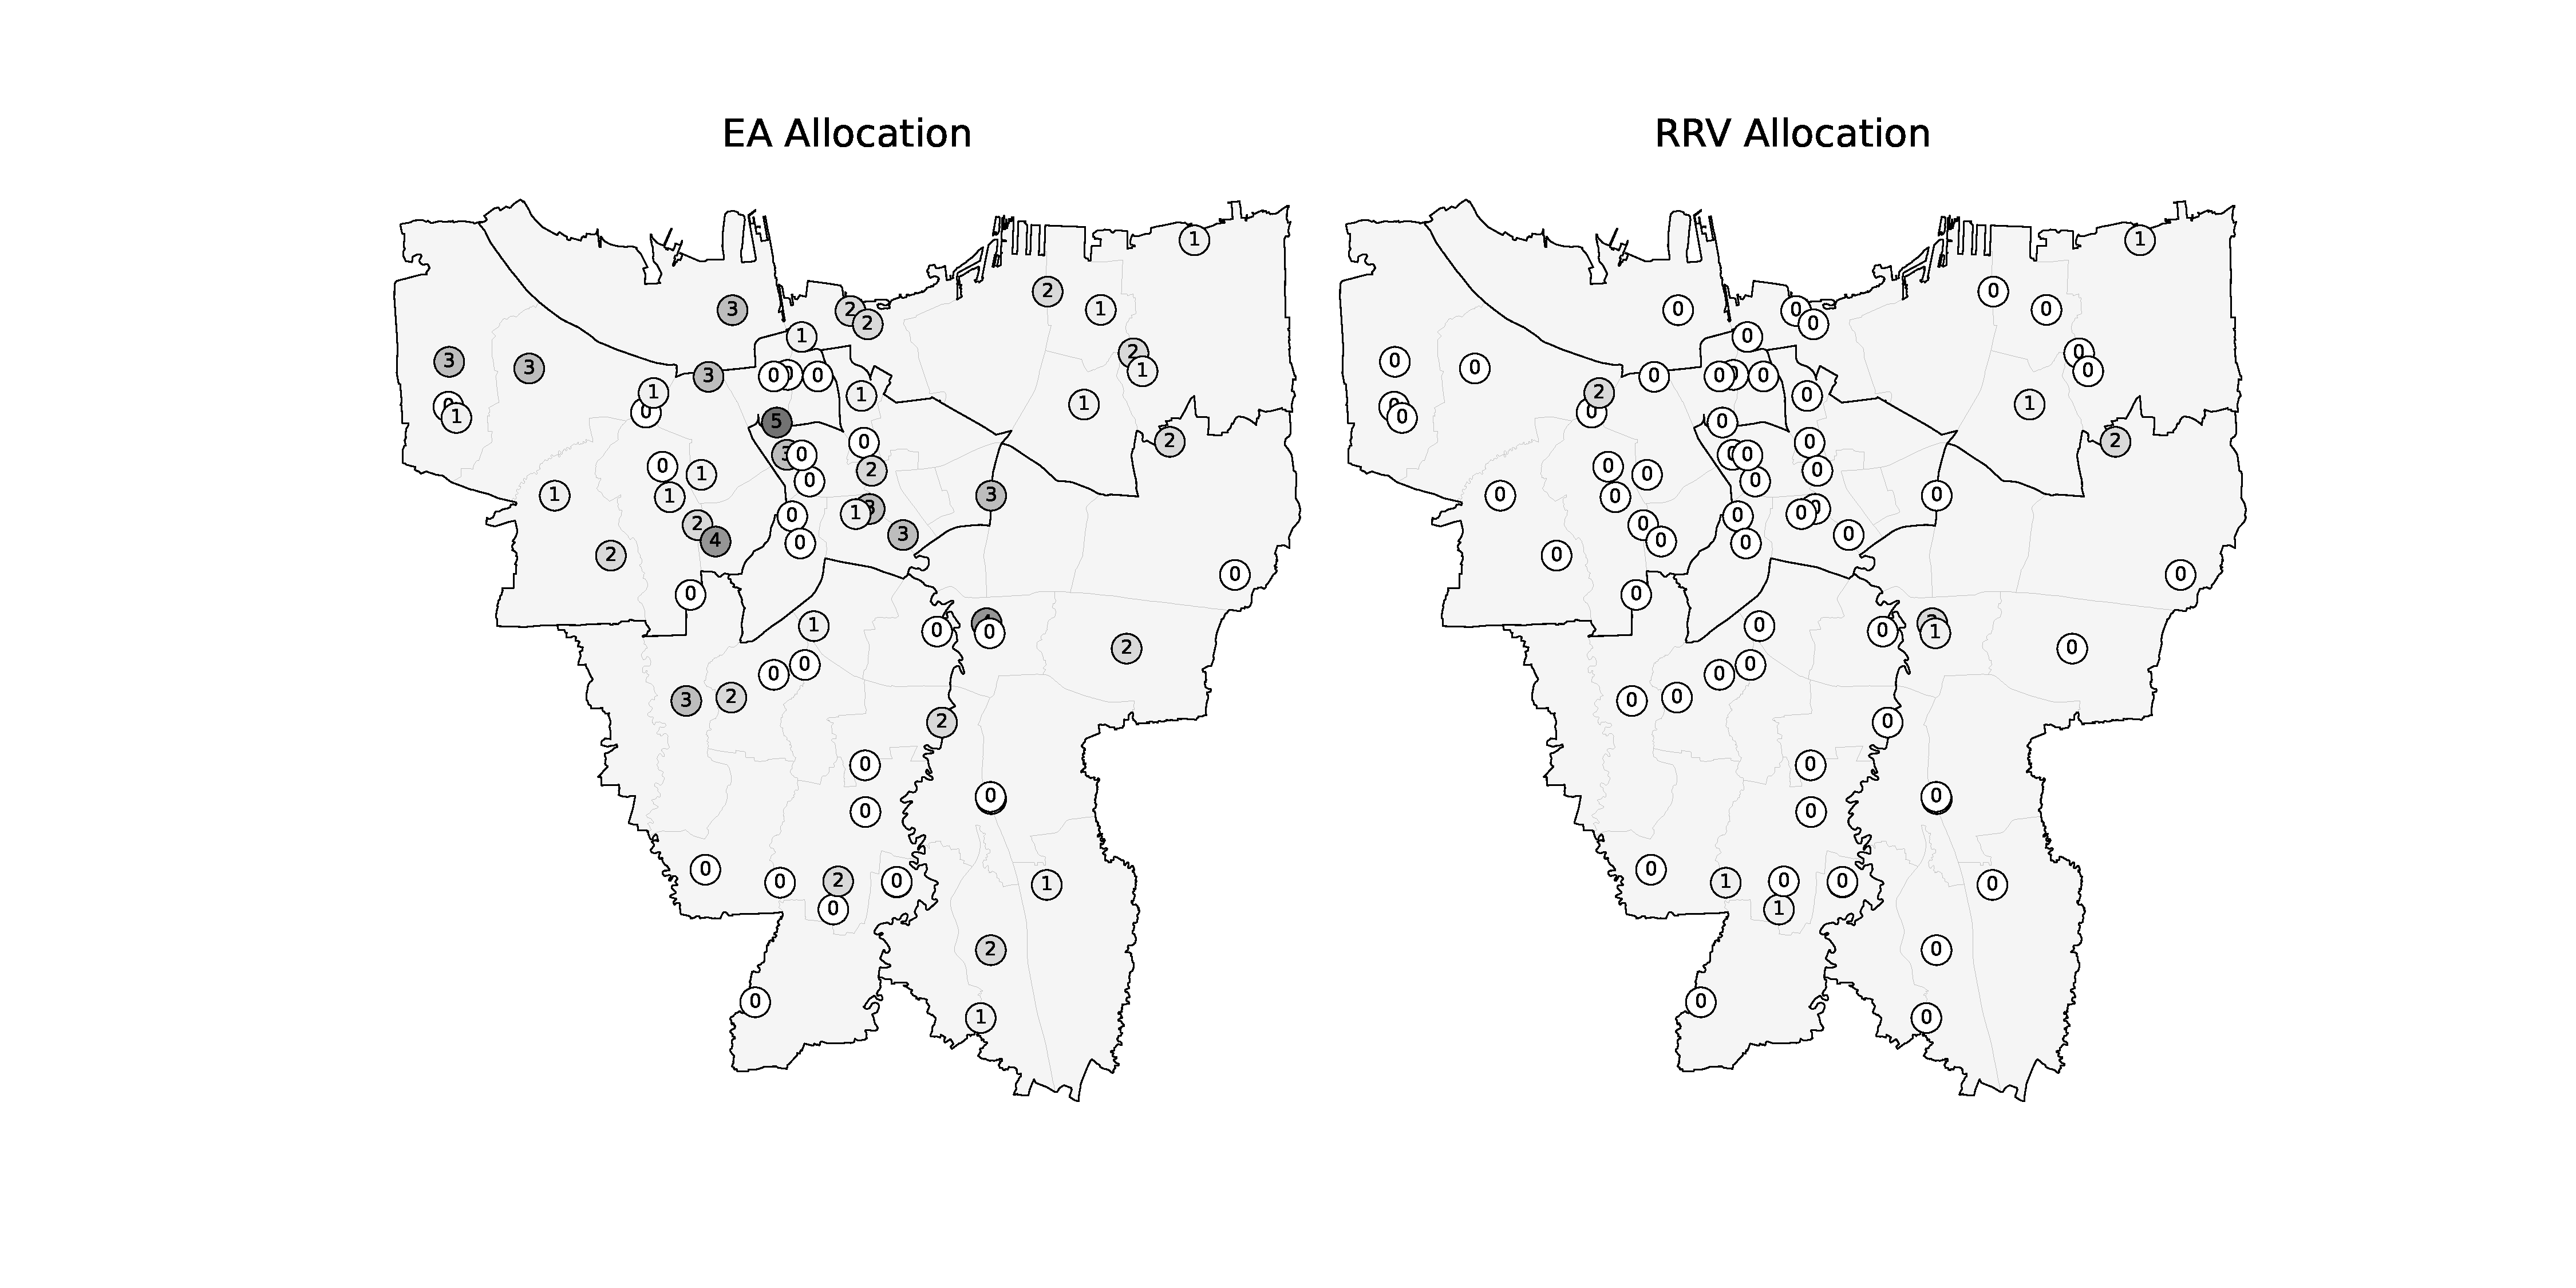
\includegraphics[width=\textwidth]{img/map_optimised_34}
\caption{Optimised allocation of 81 EAs and 13 RRVs, under scenario \textbf{D34}.}
\label{fig:optimal_current_allocation_34}
\end{center}
\end{figure}

\begin{figure}
\begin{center}
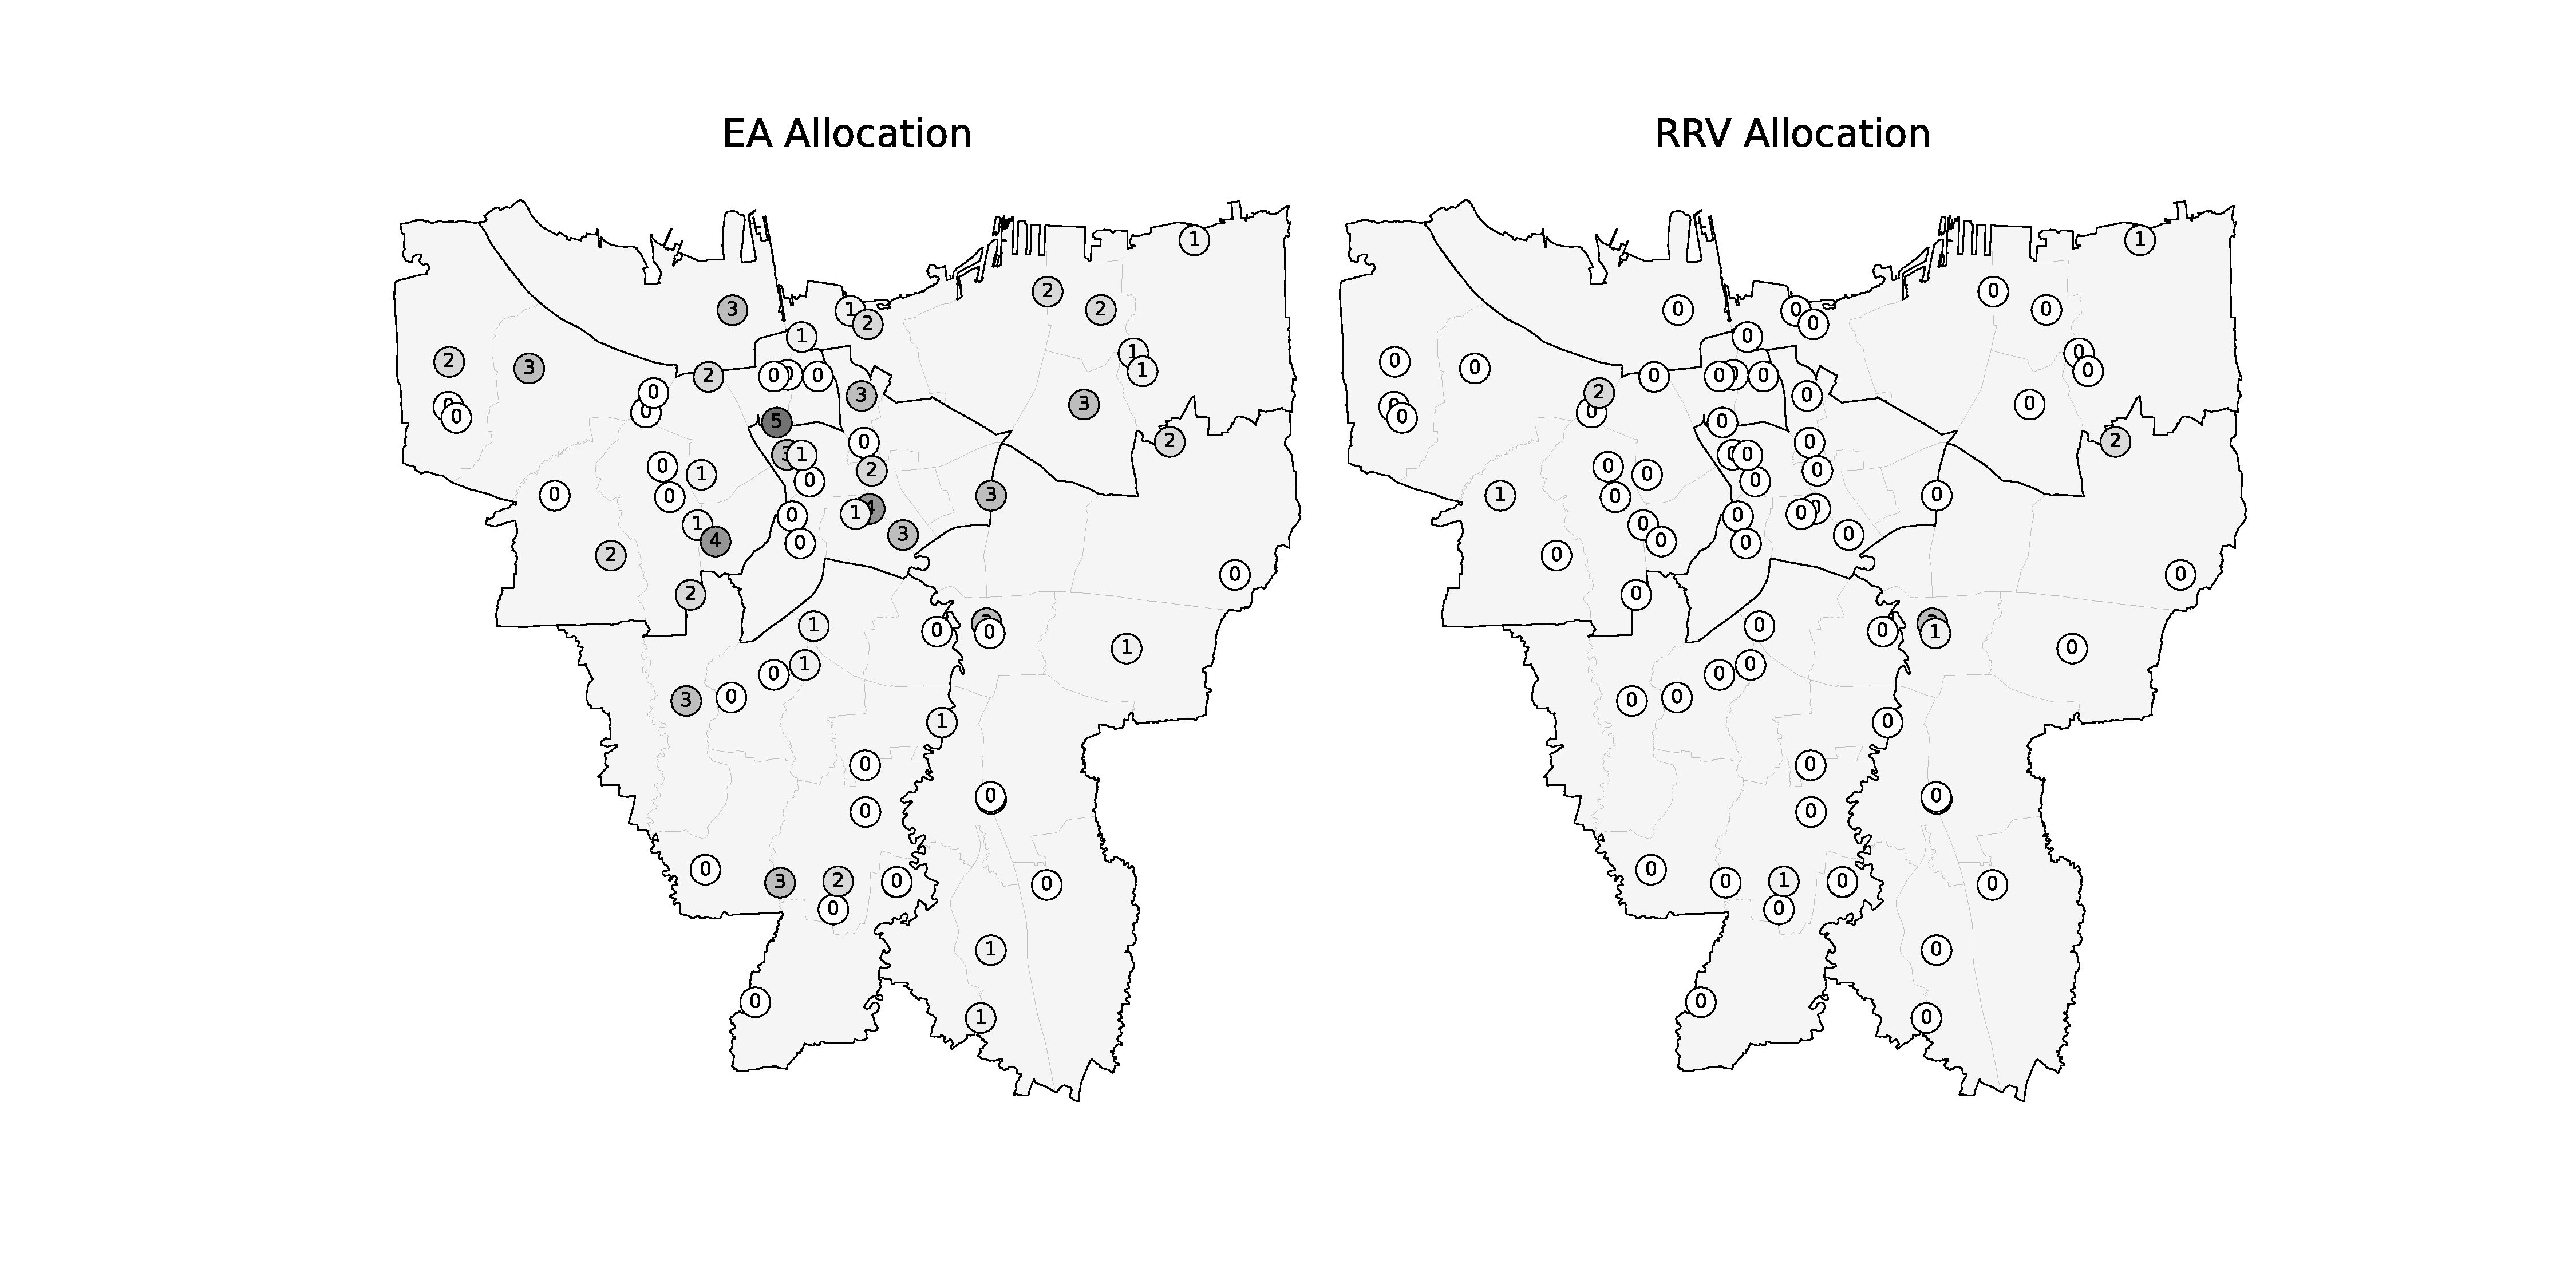
\includegraphics[width=\textwidth]{img/map_optimised_45}
\caption{Optimised allocation of 81 EAs and 13 RRVs, under scenario \textbf{D45}.}
\label{fig:optimal_current_allocation_45}
\end{center}
\end{figure}


\bibliographystyle{plainnat}
% AUTHOR: Include your bib file here
\bibliography{literature}

%\section*{AUTHOR BIOGRAPHIES}



\end{document}